\section{Introduction}
The DLR Institute for the Protection of Maritime Infrastructures (DLR-MI) is consistently working on systems to improve the situational awareness of maritime infrastructures. Part of those awareness systems is the near real-time tracking of vessels and the detection of abnormal ship behaviour. Such anomalies can potentially range from unusual trajectories, entry into restricted zones, speeding and intentional AIS on-off switching to actual collisions or pirate attacks.
\par
This thesis focuses on the construction of a system and an associated robust model that is capable of predicting accurate future vessel paths because a component like this is a promising solution in order to discover irregular ship behavior. To this extend, the ability to generate end-to-end trajectories is an advantageous addition to any maritime surveillance system which can then be utilized in a variety of different tasks, especially the detection of abnormal vessel trajectories and collision avoidance.
However, building such a sophisticated model is a challenging task because real-world ship maneuvering not only depends on movement indicators (current position, speed, heading) but also on a wide range of non-kinematic factors (e.g. weather conditions, current, tides and surrounding ships). Admittedly, only the kinematic factors are considered in this thesis due to time concerns. In addition to the potentially high-dimensional and semantically varying feature space, a suitable system has to also incorporate a time component and retain low computational costs intending to potentially provide near real-time predictions in short time intervals.
\par
Previous work at the institute regarding this topic involved the usage of sequential models like LSTMs. The downside of those network architectures is the requirement of a predefined-length frame of timestamps as input that eventually leads to a prediction of a fixed output window. An end-to-end path prediction has low performance due to the observed phenomena that sequentially taking a predicted output as input sequence leads to significant error accumulation.
\par
With the rise of deep reinforcement learning and its successful application in fields like robot control and autonomous system (\cite{s18092905, zare2021continuous, 9195789, martinsen2018curved}), the question comes to mind if this task can be formulated as a reinforcement learning problem as well. The idea behind using reinforcement learning is that training an agent to control an unmanned vessel results in a policy that learns end-to-end trajectories to get to a desired destination. While dropping the need for a dedicated simulation of the real-world, only the abstract vessel trajectories based on historical AIS records are used while forcing to agent to directly chose the speed and heading of the ship. In conjunction with extensive tweaking of the state representation and reward function, the assumption is that the agent learns to mimic normal vessel behaviour to eventually predict end-to-end trajectories.
\par
Using the word "mimic" in the previous paragraph reveals that this task is potentially better placed in the realm of \textit{Imitation Learning}, an approach that operates in the same mathematical framework as reinforcement learning and is very closely related to it. Besides an in-depth investigation of classical interactive reinforcement learning we will also heavily explore the performance when learning from expert demonstrations and trying to mimic human captain behavior.
\par
To give an example of what the agent should eventually learn, we illustrate two density maps of vessel trajectories generated by \cite{martinetraffic} for the year 2020:
\begin{figure}[H]
    \centering
    \begin{minipage}{.47\textwidth}
      \centering
      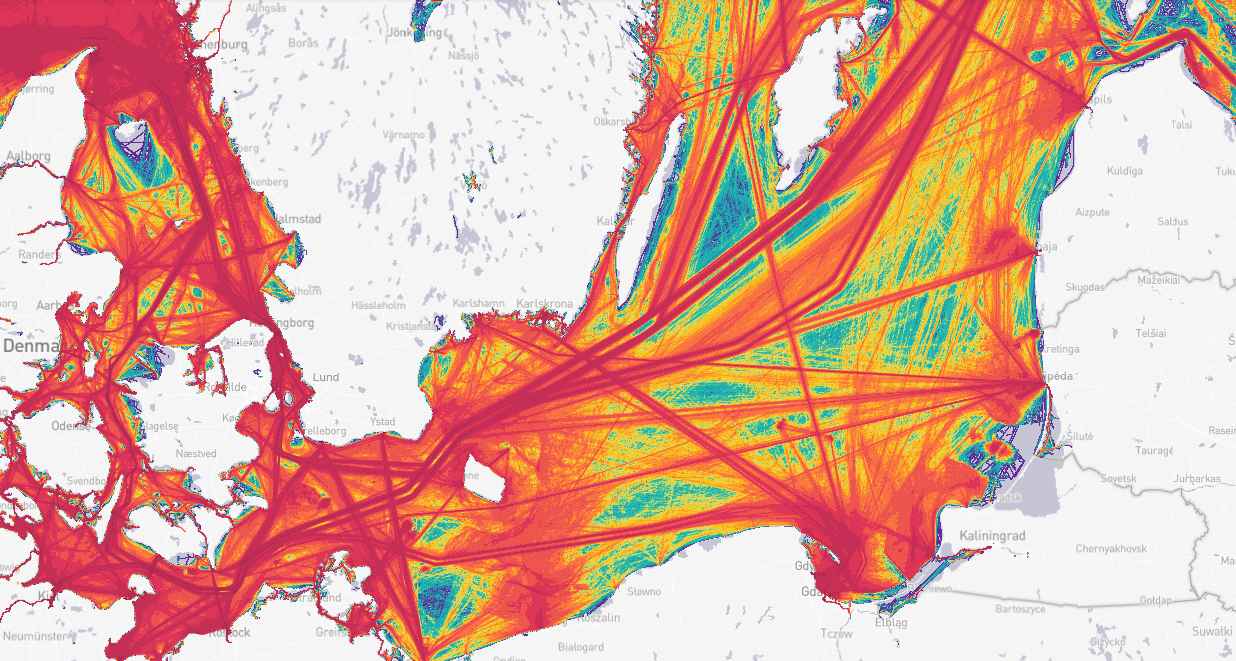
\includegraphics[width=\textwidth]{images/balticsea_density_routes.PNG}
      \captionof{figure}{Density map of vessel trajectories in the Baltic Sea}
      \label{fig:baltic}
    \end{minipage}
    \hspace{.05\textwidth}%
    \begin{minipage}{.47\textwidth}
        \centering
        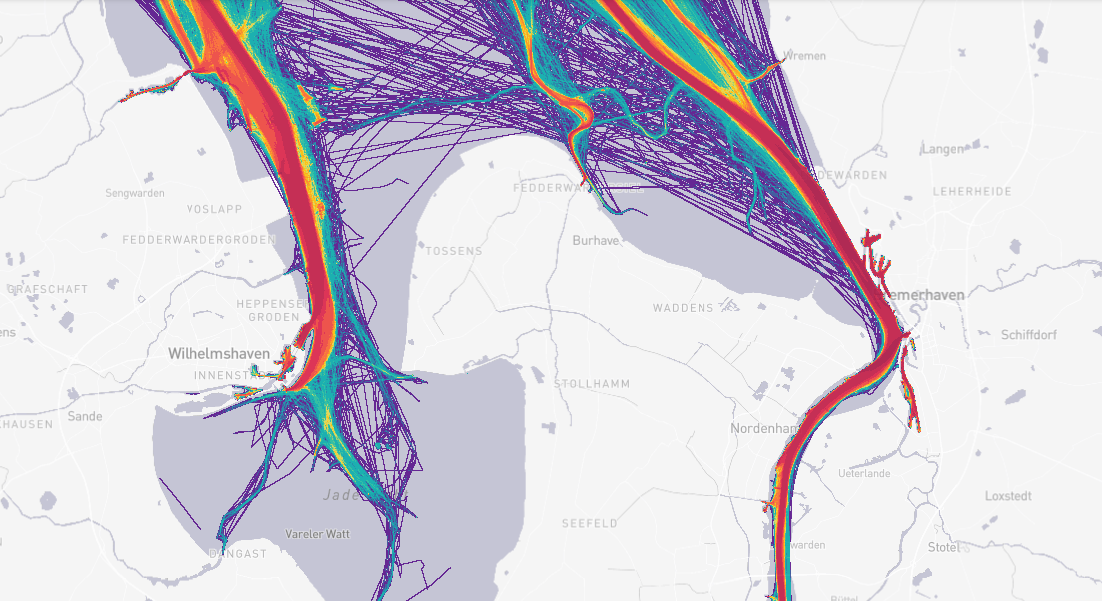
\includegraphics[width=\textwidth]{images/bhv_jadebusen_density_routes.PNG}
        \captionof{figure}{Density map of vessels near Bremerhaven and the Jadebusen}
        \label{fig:jadebusen}
      \end{minipage}
\end{figure}
Looking at Fig. \ref{fig:baltic}, we can discover the international shipping routes by following the red lines which indicate a high volume of vessel traffic. Furthermore, we notice certain points where the majority of ships choose to suddenly change their heading. It is up to the agent to learn exactly those specific patterns as in break points, entry angles to the ports, speed values etc. In contrast to the big scope of international routes in Fig. \ref{fig:baltic}, a path prediction system can also be applied to smaller more granular observation window as illustrated in Fig. \ref{fig:jadebusen}. By "granular" we mean the focus on rapid decision sequences in short time intervals when entering and maneuvering in or near a port. As the author's university and the DLR-MI is located in Bremerhaven, the observation window and scope is centered around the city's port. Fortunately, the harbour of Bremerhaven is also one of the largest ports in Europe with, for the year 2020, more than 4.7 million TEUs (twenty-foot equivalent unit) in sea goods being handled and a massive car terminal with an automobile throughput of 1.733.100 cars \cite[]{bremenports}. \label{chap:intro}
    \subsection{Objective and Requirements}
    The overall objective is the implementation of a system based on a reinforcement- or imitation learning algorithm that is able to predict end-to-end vessel trajectories based on historical AIS data. In future steps outside the scope of this thesis, the constructed model could potentially be part of an application used at a maritime surveillance center in order to push alerts e.g. in case of an upcoming close encounter between two ships if no party changes its current driving behavior. Before building a suitable system, we defined certain requirements that must be met. Those are:
\paragraph{No dedicated simulation.} Works like the one from \cite{westerlund2021learning} heavily depend on a sophisticated ship simulation to translate actual ship maneuvering like the adjustment of the current speed or rudder angle to realistic ship movements. Although open-source projects such as the \textit{Open Simulation Platform} \cite[]{smogeli2020open} are emerging, a dedicated simulation has to have the ability to reverse historical AIS data to ship controls for thousands of different vessel models because we want the system to act as closely as possible to the normal behavior of a captain approaching or leaving the Bremerhaven port. Therefore, the proposed system must be able to exclusively learn from AIS data with no explicit knowledge of the ship controls.

\paragraph{Complete end-to-end trajectories.}
Methods for predicting sequences like recurrent neuronal networks are only able to output a fixed-sized forecast window based on a fixed-sized input frame. We want the system to be flexible so it can predict complete end-to-end trajectories without the need for previous sequences. Hence, the proposed system must be able to generate full paths purely based on a single input state.

\paragraph{Real-time predictions.} The predefined system observation area as displayed in Fig. \ref{fig:systemObservation} covers approximately 300 square kilometers and thus can potentially perceive more than 50 vessels at a time. A constructed system has to have low computational costs in an effort to operate in near real-time while frequently predicting all future trajectories.


\paragraph{Extensible feature space.}
As previously described, ship maneuvering also depends on non-kinematic factors like weather conditions, tides or surrounding ships. Despite the fact that a first version does not have to incorporate those factors, it should in theory be possible to extend the system in a straight forward way.


For a better understanding of what an actual application could look like, we illustrate Fig. \ref{fig:systemObservation}.
\begin{figure}[H]
    \centering
    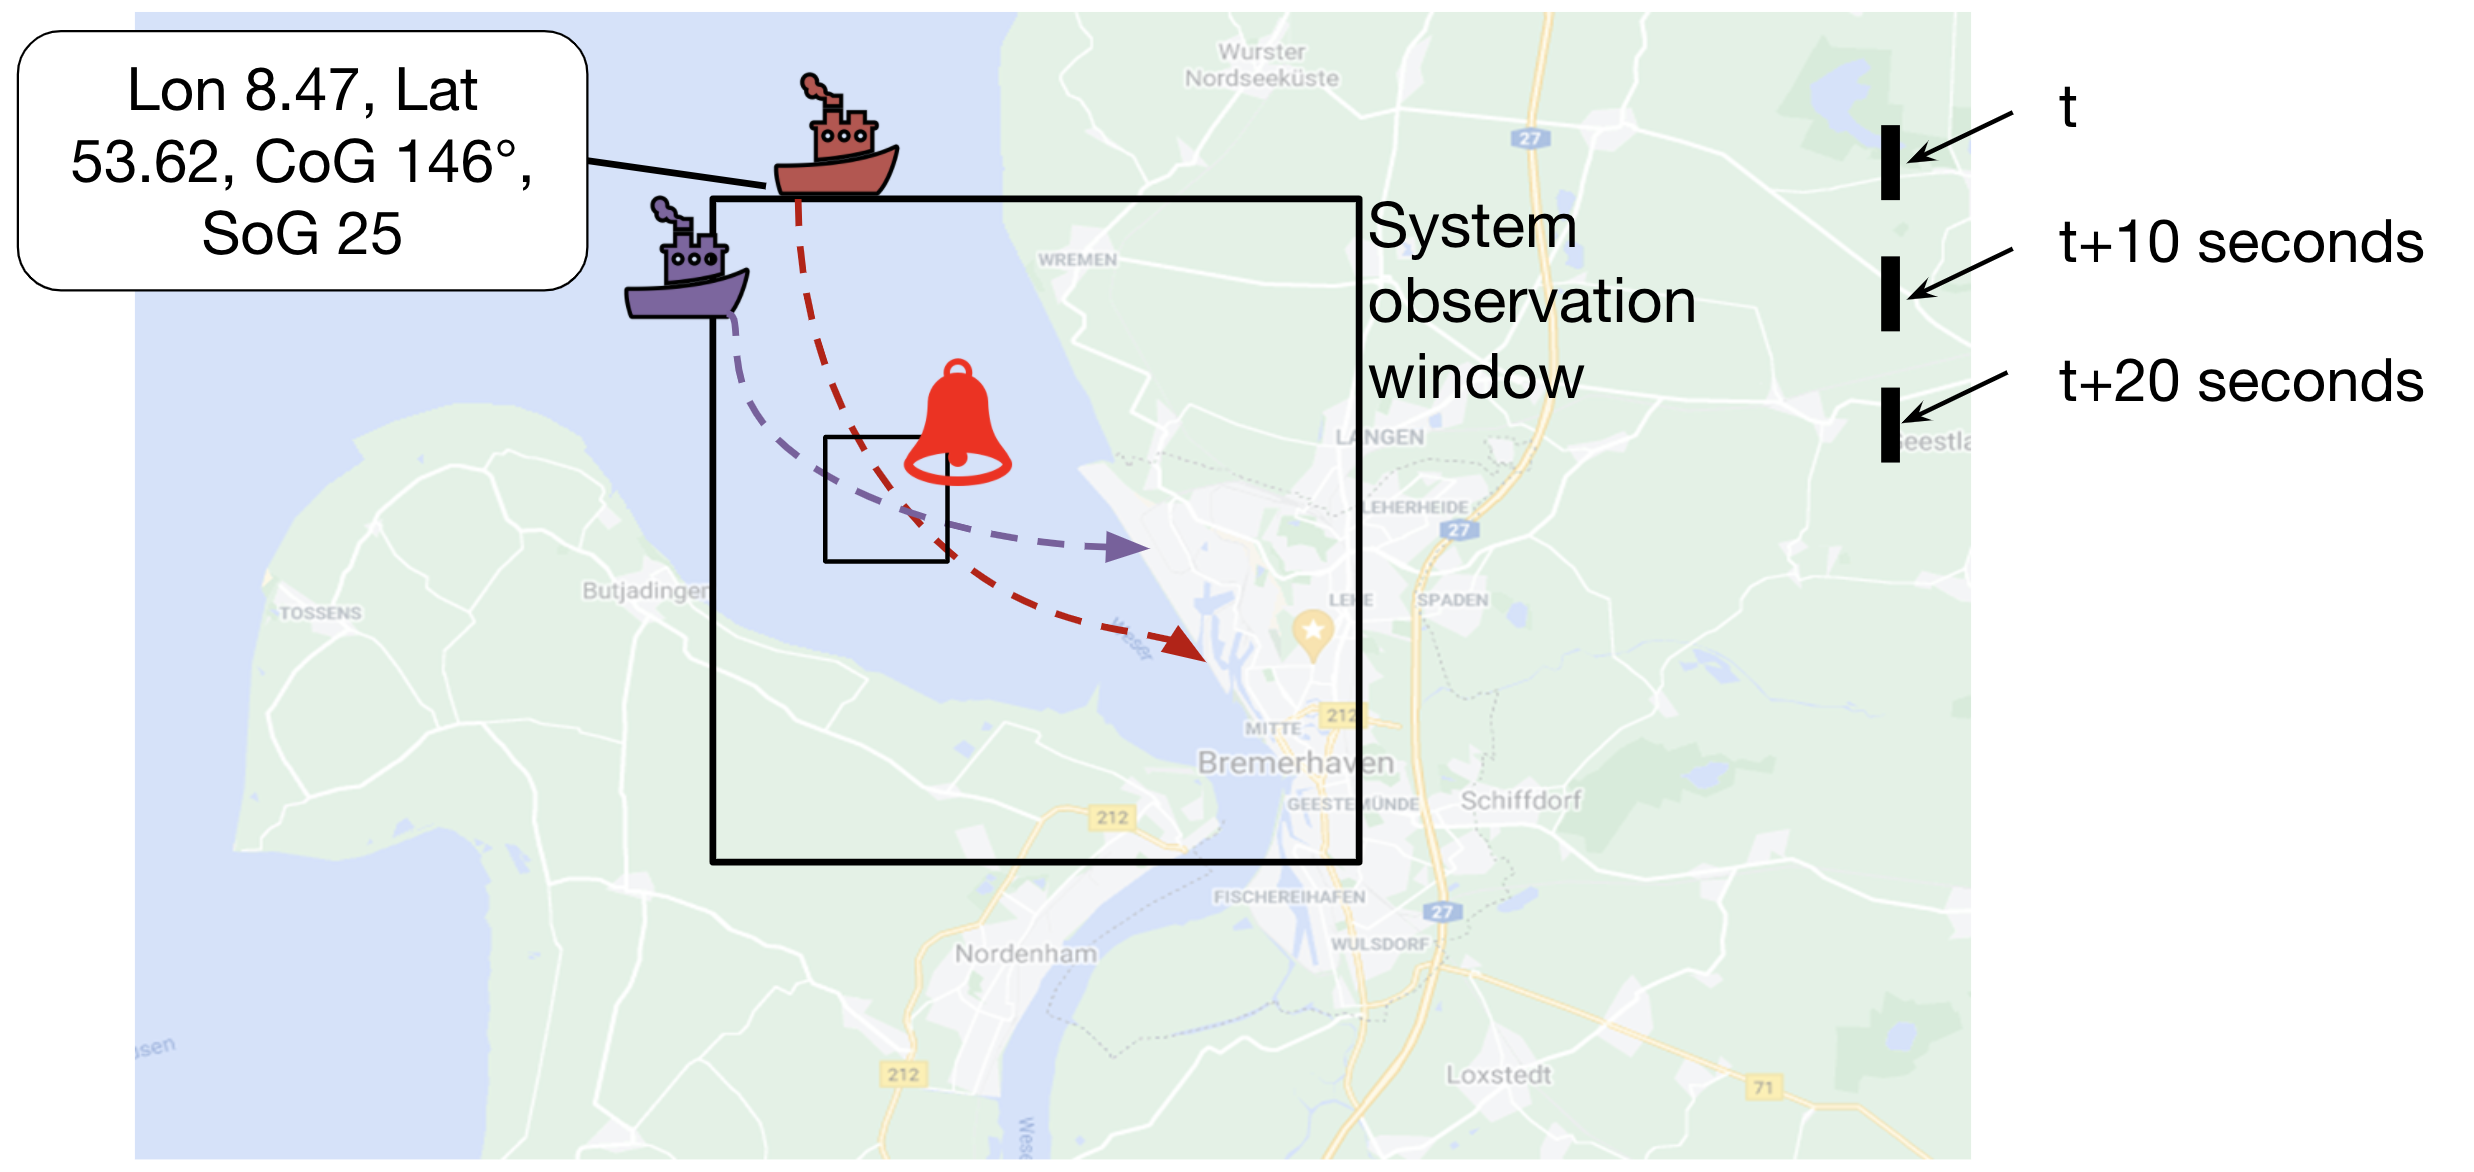
\includegraphics[width=\textwidth]{images/system_observation.png}
    \caption{System observation window.}
    \label{fig:systemObservation}
\end{figure}

The figure defines a system observation window for the port and shore of Bremerhaven. As soon as a ship enters this area, the current state with information like position, course over ground (COG) and speed over ground (SOG) is used to generate a prediction of the path a "normal behaving" instance of this ship would take. Besides drawing the raw path, the system also includes a time component indicated by the dashed line, making it possible to retrace at which specific location the ship will end up after a certain time span. Now, if another ship enters the observation area as well, both path predictions in time will be used to detect possible collisions or close encounters to then create a warning to the human operator being in charge of the marine surveillance. It is then up to the operator to contact the captains or wait for upcoming predictions to see if this incidence resolves itself.
\par
Apart from the design and implementation of the path prediction system, one intermediate goal is to get a major overview of related work in terms of the anomaly detection of vessels and the recent application of reinforcement learning, most importantly the ones regarding path planning and autonomous control. Diving deep into the field of deep reinforcement learning and imitation learning, we will also have a closer look at the internal mechanism of an actor-critic method. To improve our knowledge of state representation, feature engineering and reward function, we also set up a series of simplified experiments.
    \subsection{Motivation}
    To our best knowledge, there is no published work that takes vessel path prediction for arbitrary ship models or the generation of representative vessel trajectories based on historical AIS data into the field of reinforcement- or imitation learning. As investigation in chapter \ref{chap:relatedWork} will show, related work is focused on autonomous control with the goal to navigate unmanned ships towards a desired destination. Hence, a major part of the motivation is the study of a novel approach to the path prediction problem in the maritime domain based on reinforcement- and imitation learning to a flexible set of different ship types.
\par
Moreover, motivation arises from the significant interest of the author for the field of reinforcement learning. In his previously prepared bachelor thesis, the author has already intensively dealt with the absolute basics of reinforcement learning.  However, the investigated approaches were limited to tabular methods, which are a big restriction to the framework due to the fact that they are not suitable for complex problems with vast state and action spaces. The examination of deep reinforcement learning and the associated use of neural networks as powerful function approximation is a logical next step for the author to further educate himself in this area.
\par
In addition, an extended abstract of this work was submitted for the MARESEC 2022 workshop. This abstract was prepared in the intermediate phase of this thesis, with the plan to further refine the results by the date of the conference in Summer. The complete submitted abstract can be viewed under section \ref{appendix:maresec} in the appendix.
    \subsection{Structure}
    This master thesis is divided into four major parts. In the first part, which consists of chapters \ref{chap:prerequisites} and \ref{chap:relatedWork}, the reader is introduced to the generic reinforcement learning framework, the Automatic Identification System (AIS) and the recent developments of reinforcement- and imitation learning in general. In addition to that, a big overview is shown in chapter \ref{chap:relatedWork} which also presents different methods and approaches aside from reinforcement learning.
\par
After finishing the first part and chapter \ref{chap:relatedWork}, the next part deals with the functioning and general assumptions of the algorithms and methods used in this thesis on a very theoretical level. Chapter \ref{chap:DDPG} dives deep into the inner workings of a popular reinforcement learning algorithm based on the actor-critic architecture, DDPG, whereas chapter \ref{chap:imitation} presents an entirely different approach to the overall task as in directly mimicking the expert's behavior and argues why imitation learning is a better choice.
\par
The third part and chapter \ref{chap:synthetic} constructs a synthetic, simplified version of the real-world environment in order to investigate the performances of different experimental setups with different state spaces, algorithms, and hyperparameters. Findings and assumptions are then used in the next part, the building of the actual prediction system based on historical AIS data. In this chapter \ref{chap:realworld}, the whole process of extracting vessel trajectories, defining different training sets, running experiments, evaluation as well as failure tracing and the proposal of possible improvements take place. In the end, conclusions are drawn in chapter \ref{chap:conclusions}.
    
\newpage
\section{Prerequisites}\label{chap:prerequisites}
    \subsection{RL Framework}\label{chap:rlframework}
    In a reinforcement learning setup an agent is interacting with an environment $E$ at discrete time steps. At every time step $t$ the agent observes the current state of the environment $s_t$ and selects an action $a_t$. Feedback is returned by the environment in the form of a scalar reward $r_{t+1}$ and the resulting state $s_{t+1}$ based on the internal dynamics of the environment. We will use the definitions of \cite{Sutton1998} throughout this chapter, especially the definition of the point in time the reward is given back. In contrast to other publications like those from \cite{zare2021continuous}, \cite{wiering2012reinforcement} and \cite{lillicrap2019continuous}, \cite{Sutton1998} do not bind the reward signal to the same time step as the current state-action pair ($s_t$, $a_t$) but rather the next one, to indicate that the reward and the next state are calculated at the same time $t+1$.
This interaction can thus be illustrated in the following way, where the uppercase symbols $A$, $S$, and $R$ are used to indicate random variables. Their concrete instances of states, actions, or rewards are specified by the corresponding their lowercase symbols (e.g., $s_t$, $s_{t+1}$, or $a_t$):
\begin{figure}[H]
    \centering
    \hspace*{1cm}%
    \begin{tikzpicture}[]
\node (A) at (3,3) [rectangle, rounded corners, draw, minimum height=1cm,minimum width=3cm] {Environment};
\node (B) at (3,0) [rectangle, rounded corners, draw, minimum height=1cm,minimum width=3cm] {Agent};

\node (C) at (0.7, 3) [rectangle, thick, dashed, inner sep=0pt, minimum height=1cm, minimum width=0cm, draw] {};

\draw[->, black, very thick] ($(B.east)$) to[out=0,in=0, distance=2.5cm] ($(A.east)$);

\draw[->, black, very thick] ($(A.west)-(0.1,0)$)  to[out=3,in=7] ($(C.east) -(0,0.02)$);

\draw[->, black, very thick] ($(C.east) - (0,0.02)$) to[out=193,in=180, distance=2.4cm] ($(B.west)$);

\node[text width=3cm] at (1.6 , 4) 
    {$R_{t+1} S_{t+1}$};
    
\node[text width=3cm] at (-1.6 , 0.8) 
    {Observation \\ $S_t$};

\node[text width=3cm] at (-1.6, 2.2) 
    {Reward \\ $R_t$};
    
    
\node[text width=3cm] at (8.3, 1.5) 
    {Action \\ $A_t$};
    
\end{tikzpicture}
    \caption{Agent-environment interaction.}
    \label{fig:rlEnvironment}
\end{figure}



To be precise, we formalize the environment as a Markov decision process (MDP) with state space $\mathcal{S}$, continuous action space $\mathcal{A}$ , the transition dynamics $p(s_{t+1} \mid s_t, a_t)$ and reward function $r(s_t, a_t)$. The reward function is hand-crafted and indicates whether the selected action in a certain state is considered "good" or "bad". The action selection process or rather the \textit{behavior} of the agent is defined by a policy $\pi$, which is essentially a mapping from states to probabilities of actions being chosen $\pi: S \rightarrow P(A)$. But as we will exclusively calculate deterministic policies in this thesis, we define $\pi: S \rightarrow A$.
\newpage
One of the major challenges arises from the nature of an MDP being a sequential decision problem. An action that seems to be mediocre in the present may result in a trajectory that produces better rewards in the long run and vice versa. It is therefore necessary to take future rewards into account. The discounted sum of future rewards is called the \textit{return} with a discounting factor $\gamma \in (0,1]$  \cite[p.55]{Sutton1998}:

\begin{equation}\label{eq:discountedReturn}
    G_t = R_{t+1} + \gamma R_{t+2} + \gamma^2 R_{t+3} + \dots  = \sum_{k=0}^\infty{\gamma^k R_{t+k+1}}
\end{equation}

By reshaping the above equation, we can discover the relationship between consecutive returns \cite[p.55]{Sutton1998}:
\begin{equation}\label{eq:successiveReturn}
    \begin{aligned}
    G_t &= R_{t+1} + \gamma R_{t+2} + \gamma^2 R_{t+3} + \gamma^3 R_{t+4} + \dots \\
    &= R_{t+1} + \gamma (R_{t+2} + \gamma R_{t+3} + \gamma^2 R_{t+4} + \dots)  \\
   & = R_{t+1} + \gamma G_{t+1}
    \end{aligned}
\end{equation}

The overall objective of a reinforcement learning agent is therefore to find an optimal policy that maximizes the return for a given starting state $s_0$. In order to do so, reinforcement learning algorithms estimate the expected return for any given state or state-action pair, which is also called the \textit{value} or $Q$-value. The recursive relationship revealed in equation \ref{eq:successiveReturn} naturally applies to $Q$-values as well, which is formally described by the \textit{Bellman equation} (for discrete policies):

\begin{equation}
    Q^\pi(s_t, a_t) = \EX_\pi[r(s_t, a_t) + \gamma Q^\pi(s_{t+1}, \pi(s_{t+1})]
\end{equation}

Unfortunately, it is impossible to solve this equation if the model of the environment is unknown. Even if a perfect model is present, methods like \textit{Dynamic Programming} have limited utility due to their great computational expense \cite[p.~73]{Sutton1998}. Therefore, reinforcement learning algorithms take an iterative approach by interacting with the environment, sampling feedback and consecutively updating estimates of the actual returns. The closer those estimates are to the real values, the better the derived policy because the greediest policy will just select the action with the highest $Q$-value for every state.
\par
Tabular methods, as the name suggests,  keep all state-action pairs and their corresponding $Q$-value in big tables, updating them if needed. In contrast, deep reinforcement learning techniques utilize powerful function approximators like neuronal networks for the purpose of replacing the memory-limited tables and handling huge state and action spaces.
    \subsection{Automatic Identification System}
    This subchapter explains the underlying communication system that produces the historical ship trajectory data which in return acts as ground truth during learning representative vessel paths. Giving a broad overview of the standard, this chapter is meant for readers that are not familiar with the domain of maritime traffic.
\par
To ensure and enhance maritime safety, ships are constantly broadcasting information about their current position, speed, course etc. At the same time, they are receiving the broadcasts from all other ships around them, resulting in a superior understanding of the situation in order to, e.g, avoid collisions. 
\par
The whole system behind exchanging those ship information is summarized under the term \textit{Automatic Identification System} (AIS). In 2000, the International Maritime Organization (IMO) which is a specialized agency of the United Nations responsible for regulating shipping, made it mandatory for a list of ship types to carry an AIS \cite[]{imo}. This list includes ships 
with more than 300 gross tonnage (international voyages), cargo ships with more than 500 gross tonnage and all passenger ships irrespective of size \cite[]{imo}.
\par
All intentions, specifications, and regulations regarding AIS are documented in the official and revised \textit{Guidelines for the Onboard Operational Use Of
Shipborne Automatic Identification Systems (AIS)} \cite[]{international2015revised}. These guidelines also mention the objectives for AIS to be the:
\begin{itemize}
    \item identification of ships and assistance in target tracking
    \item simplification of the information exchange (e.g., reduce verbal mandatory ship reporting)
    \item help of port authorities or other shore-based facilities to enhance situation awareness
    \item assistance in search and rescue operations
    \item avoidance of ship collisions
\end{itemize}

The content of an AIS message depends on the type of the information. There are three different types that can be transmitted, specifically static-, dynamic- and voyage-related information. In this context, static information are defined per vessel and include the \textit{Maritime Mobile Service Identity} (MMSI) which is unique for every ship as well as other ship dependent information such as length and type of ship. A list of all ship types can be found in the official installation guide of AIS, published by \cite{imo2}. In this thesis we will mainly focus on ship types that have a 6 (passenger), 7 (cargo) or 8 (cargo) as first digit while ignoring type 52 (tugs) because of their very distinct maneuvering.
\par
Voyage-related information should in theory consist of the ship's draft, the cargo type, the destination, and ETA as well as a route plan. However, those data points have to be entered manually and thus are suffering from high variance not only in availability but also credibility. Although, the knowledge about the destination could be a valuable attribute, especially if it comes down to the distinction of certain vessel paths, we will ignore all voyage-related information.
\par
Besides the static- and voyage-related information which is broadcasted every 6 minutes or upon request, the dynamic information mainly consist of kinematic data that gets send out every 2 to 10 seconds depending on the ship type and the current speed and course alteration. If a ship is at anchor, the reporting interval is extended to 3 minutes. The content of a dynamic AIS message includes the position given by latitude and longitude, a UTC timestamp, speed over ground (SOG) and course over ground (COG), the heading of the ship, the current navigational status (underway by engines, at anchor, engaged in fishing etc.) and the rate of turn (ROT). 
\par
The values for all of those data points are collected from ship sensors that are connected to the AIS. Therefore, the IMO warns that "poorly configured or calibrated ship sensors (position,
speed, and heading sensors) might lead to incorrect information being transmitted" \cite[p.~11]{international2015revised}. They also state that the accuracy indication of the position is approximately 10 meters (p.~6).
    \subsection{Recent Developments and Achievements}
    This sub chapter gives an overview of the latest developments and achievements in the research field of deep reinforcement learning, starting with the key paper that is responsible for the re-ignition and the explosion of interest in reinforcement learning, the work from \cite{mnih2013playing, mnih2015human}.
\par 
\cite{mnih2013playing} propose an algorithm called Deep Q-Network
(DQN) that combines Q-Learning with a neural network which is used to estimate the Q-values instead of using a look-up table. One of the reasons the paper got so much attention is due to the fact that the algorithm learned to play seven Atari games on human like level just based on the pure pixel input without changing the architecture (p.~7-8). The main difference between the presented method by \cite{mnih2013playing} in contrast to past approaches of using neural networks in conjunction with reinforcement learning, is the introduction of an experience replay and a target network to ensure stability during the training process. We go into detail on those components later in this thesis.
\par
Four years after the initial publication of DQN, \cite{hessel2018rainbow} combine the suggested improvements to DQN by the research community to propose an algorithm called \anf{Rainbow}. Although DQN and Rainbow can be seen as milestone methods, they are still only capable of handling discrete action spaces. Instead of estimating Q-values, policy gradient methods represent the policy by a parametric probability distribution that either stochastically or deterministically selects an action. Those methods are used to be able to operate in the continuous action space as this is often a mandatory requirement for example in robotic control. Examples for algorithms that are labeled as the stochastic case are Proximal Policy Optimization (PPO) \cite[]{schulman2017proximal} and Trust Region Policy Optimization (TRPO) \cite[]{schulman2017trust}.
\par 
A deterministic policy gradient (DPG) algorithm was first introduced by \cite{silver2014deterministic} who propose an off-policy algorithm based on the actor-critic framework. We will go into detail about this approach in another chapter of the thesis. One year after the DPG paper got published, \cite{lillicrap2019continuous} combined the DPG method with the stability mechanisms presented in the DQN paper, to great success. As we will see in the next chapter that focuses on related work, nearly all efforts that involve  a control problem in the continuous action space utilize the improved version of DPG which is also referred to as DDPG \cite[p.~2]{lillicrap2019continuous}. The latest major accepted algorithm that is built on top of DDPG and tries to improve it, is the Twin Delayed Deep Deterministic Policy Gradient (TD3) algorithm \cite[]{fujimoto2018addressing}. Besides, there exists an algorithm named Soft Actor-Critic (SAC) suggested by \cite{haarnoja2018soft} that combines the actor-critic framework of DDPG with a stochastic actor.
\par
As we noticed in the previous explanations and also in OpenAI's key paper list \cite[]{keypaperlist}, the release of milestone papers regarding the algorithms themselves stopped around 2018. The question arises as to what the main research topic trends were in the past three years because the overall hype around reinforcement learning certainly did not stop yet as the number of publications display - 1302 in 2018, 2140 in 2019 and 3256 in 2020 \cite[]{arxiv}. During our literature research, we notice an emerging trend towards offline reinforcement learning and the strive to make reinforcement learning methods more data efficient. \cite{levine2020offline} provide the research community with a great conceptual overview of the topic as a whole, including difficulties and open problems, while \cite{fu2021d4rl} introduce special data sets that are designed for benchmarking. \cite{fujimoto2019benchmarking} apply multiple offline reinforcement learning algorithms to the Atari game playing domain to compare the results to the original proposed DQN algorithm. All offline reinforcement learning algorithms are under-performing in comparison to the online DQN with the strongest one being a discrete variant of Batch Constrained deep Q-Learning (BCQ) \cite[pp.~7-9]{fujimoto2019benchmarking}. Although offline reinforcement learning methods should learn an improved policy derived from the original behaviour policy that sampled the data, BCQ is only able to match it and thus can be seen as robust imitation in this Atari setting \cite[pp.~7]{fujimoto2019benchmarking} which is not the desired outcome.
\par
However, imitation in general plays a major role in hard exploration problems in which agents are unable to find even one successful decision sequence after billions of training steps. One example being the task of autonomous driving. \cite{le2022survey} describe in their related survey that applying imitation learning, a method of learning from expert (human) demonstrations, is more applicable to the driving task due to the complexity and safety critical nature (p.~1). The authors also list a wide range of related works which in return utilize  constantly evolving methods of the realm of imitation learning (pp.~10-13). An overview of the advances of imitation learning can also be found in the paper proposed by \cite{zheng2021imitation}. Starting from one of the simplest approaches in the form of behavioral cloning which is also a core method used in this thesis, the authors also mention the latest developments of the three categories and their first presented algorithms, namely behavioral cloning \cite[]{alvinn}, direct policy learning (Generative Adversarial Imitation Learning (GAIL) \cite[]{ho2016generative}) and inverse reinforcement learning (Adversarial Inverse Reinforcement Learning (IRL) \cite[]{fu2017learning}). Some improved methods based on those three are e.g. CMILe \cite[]{tu2021closing}, DGAIL \cite[]{zuo2020deterministic} and SQIL \cite[]{reddy2019sqil}. Besides, works such as the ones from \cite{paine2019making} and \cite{hester2017deep} combine the imitation aspect with the previously described DQN (learn to play Atari games based on pixel input) by suggesting methods called  Recurrent Replay Distributed DQN from Demonstrations (R2D3) and Deep Q-learning from Demonstrations (DQfD) respectively.
\par
A totally different approach is used in the recent work by \cite{chen2021decision} who abstract the reinforcement learning task as a sequence modeling problem and utilize the transformer architecture to eventually output the optimal actions. This shows the flexibility of the reinforcement learning framework and the underlying MDP because RL can easily be combined with all sorts of current state-of-the-art network architectures like transformers, GANs, CNNs, LSTMs etc. Especially the usage of transformers for the overall task of this thesis, the path prediction, might also be worth an investigation since works like the one from \cite{giuliari2021transformer} show their potential in forecasting (pedestrian) trajectories.
\par
Another focus of latest research is the ability to extract features and learn directly from raw pixel input, dropping the need for manual feature extraction to shape the perfect state representation. \cite{srinivas2020curl} present a method called Contrastive Unsupervised Representations for Reinforcement Learning (CURL) that outperforms Rainbow (improved version of DQN) in the Atari domain by 30\% and almost matches the performance of SAC in the \textit{DM Control} environment which is not using raw pixel as input in contrast to CURL \cite[p.~7]{srinivas2020curl}. Displaying the fast pace in which research in the field of RL is done, it only took 20 days for \cite{kostrikov2021image} to relativize the achievements of CURL by showing that data augmentation is in fact the key to applying strong model-free algorithms like SAC to the task of learning from raw pixel input.
\par 
Last but not least there are aspirations to make reinforcement learning scale 
better on multi-machine-setups with one example being the framework IMPALA (Scalable Distributed Deep-RL with Importance Weighted
Actor-Learner Architectures) proposed by \cite{espeholt2018impala}.
\newpage
\section{Related Work}\label{chap:relatedWork}
After a profound literature research, we can divide the related work into two sub categories. Those include the topics of building a framework for anomaly detection in the maritime domain and the general application of machine learning in path planning or prediction.

%different approaches to reinforcement learning such as inverse- and offline reinforcement learning and the ongoing work done in the field of deep reinforcement learning.
\par 
\paragraph{Anomaly detection of vessel behaviour}
Building a maritime awareness system that operates in near real time by processing huge amounts of data from all kinds of different sources (AIS, radar systems, satellites, etc.) is not a trivial task. The work of \cite{tsogas2019geospatial} presents a system architecture named Geospatial Complex Event Processing Service (TRITON) that is capable of handling large volumes of incoming events using ActiveMQ as message broker and PostgreSQL as database which is optimized for storing and querying geospatial information. By using the Event Processing Language (EPL), the service is also able to detect abnormal vessel behaviour. Though the set of specific rules (vessel entering, exiting, crossing, moving away or approaching areas) have to be defined by domain experts \cite[p.~4]{tsogas2019geospatial} which is a critical limitation of the detector. The authors themselves are thus mentioning the usage of reinforcement and unsupervised learning in future work \cite[p.~9]{tsogas2019geospatial}.
\par 
The general approach of using geospatial data like AIS to learn motion patterns, that are eventually used to predict vessel paths and detect anomalies, is not a novelty. Instead of employing hand crafted rules, the highly cited work by \cite{ristic2008statistical} uses historical AIS data to extract motion patterns to train an anomaly detector by applying statistical methods such as adaptive kernel density estimation and particle filters. A motion pattern in this connection is defined by kinematic information including ship location and velocity but also by at least one mandatory attribute information - the ship's origin - to distinguish between overlapping motion patterns \cite[p.~2]{ristic2008statistical}. This could be an interesting factor when designing a suitable state representation to fulfill the Markov property.
\par 
In a recent summary of the related literature, \cite{zhang2020analysis} analyze the research trends of vessel abnormal behavior detection of the past ten years. They found that earlier work concentrated on the detection of just abnormal tracking positions mainly based on statistical methods by almost exclusively using movement data (position, speed, heading) of the perspective of a single ship (pp.~47-48). In contrast, more recent approaches try to detect anomalies in specific situations by including contextual information such as meteorological data, the interaction between ships, the perception of ship motion status (identification of fishing operations, ship towing push or ship gathering) and video data \cite[p.~50]{zhang2020analysis}. The usage of non-kinematic features should therefore be deflected to eventually construct a sophisticated anomaly detector that  truly has a sense of situational awareness. In their work, \cite{zhang2020analysis} conclude that detectors of abnormal vessel behaviour face major problems, such as poor comprehensiveness (cannot specify abnormality type and degree), difficulties with huge amounts of data due to the complexity of their algorithms and high false alarm rates because of subjectively chosen thresholds (p.~52).
\par 
As mentioned in chapter \ref{chap:intro}, the term \anf{anomaly} can mean many things even in the conjunction of AIS data. Detecting abnormal vessel behaviour solely based on the trajectory is the main focus of this thesis but there are other types as well. \cite{singh2020effectiveness} who are colleagues at the sister institute in Neustrelitz, near Berlin, focus on malicious and intentional AIS on-off switching (OOS) anomalies. In their paper they compare the performance of various AI techniques including support vector machines, k-nearest neighbours, decision trees, artificial neural networks and naive Bayesian towards detecting the AIS
OOS anomalies using real historical AIS data (p.~1). The results (99,9\% accuracy when using an artificial neural network \cite[p.~7]{singh2020effectiveness}) suggest that this specific task can be labeled as solved. 


\paragraph{Path prediction}
To predict the trajectories of vessels, \cite{liu2019vessel} use support vector regression (SVR) in conjunction with an algorithm called ACDE for  parameter optimization. ACDE stands for \anf{differential evolution based on adaptive control parameters} and is an improved version of the differential evolution algorithm which tackles stochastic parallel optimization and is based on evolutionary ideas in form of genetic algorithms \cite[pp.~1-3]{thangaraj2009simple}. In their work, \cite{liu2019vessel} also present algorithms on how to extract single trajectories from the AIS data using the unique maritime mobile service identification (MMSI) numbers and how to clean, de-noise and normalize the AIS data (pp.~9-11). As multivariable input or in the context of reinforcement learning this can also be called \textit{state}, the authors of this paper are using unix timestamps, longitude, latitude, course and speed over ground of the ship (p.~11). We can redefined their input as state definition for a better overview, where $COG_t$ and $SOG_t$ are course and speed over ground respectively:
\begin{equation}
S_t = \{lon_t, lat_t, COG_t, SOG_t, Unix_t\}
\end{equation}
Four of those previous states plus the timestamp of the next moment $T_{t+1}$ will be the true input for two separate SVR models, one predicts the longitude $lon_{t+1}$ and the other predicts the latitude $lat_{t+1}$ for just one moment in advance \cite[p.~11]{liu2019vessel}. Predicting just the next timestamp in advance, this method might be not suitable in terms of forecasting a complete vessel trajectory because of the major concern that this model will accumulate error if a prediction output is used as input for a larger forecasting window.
\par
In a recent published paper, \cite{venskus2021unsupervised} tackle the exact same topic of this thesis, that is the prediction of vessel trajectories based on historical AIS data in an unsupervised manner. They use an LSTM autoencoder that learns to reconstruct vessel paths for the next $X$ timestamps (p.~724). Furthermore the authors utilize a method proposed by \cite{cruz2019} to eventually generate a prediction region that is learned by two supplementary LSTM autoencoders in addition to the  most like-hood forecast of the original autoencoder that learns single trajectories (p.~725). Predicting a potential region that vessels under normal behavior would navigate in, makes anomaly detection trivial by just checking if the prognosticated path is inside the region that is considered \anf{normal}. Nevertheless a major constraint of this method is the needed input sequence of past $X$ timestamps to start forecasting the next $X$ timestamps.
\par 
\cite{perera2012maritime} introduce a framework to monitor maritime traffic by constructing three modules. The first module consists of an artificial neural network that detects and tracks multiple vessels while the second and third modules are used to estimate the vessel states and forecast the navigational trajectory by using an extended Kalman filter \cite[p.~1]{perera2012maritime}. 
\par 
A complete different approach is presented by \cite{6198334} who take advantage of the genetic algorithm in conjunction with randomly generated Bezier curves to solve the path planning of  autonomous unmanned aerial vehicles (UAVs) in previously defined environments~(p.~1). Besides they achieve quasi-linear speedup in relation to the number of CPU cores by using a parallel programming paradigm called \anf{single-program,
multiple-data} (pp.~7-8). Although the authors themselves state that the planning takes 10 seconds while running on eight cores in parallel, they still make the conclusion that \anf{real-time path planning for UAVs is possible} \cite[p.~9]{6198334}. However, we see this computational cost as critical limitation of classic genetic algorithms in general. Even though vessel planning cuts one dimension as the prediction of UAVs paths takes place in a 3D domain, we still make the assumption that this approach is not suitable for future visions of calculating vessel paths of hundreds of ships in near real-time. 
\par 
Entering the field of deep reinforcement learning, we can notice that most works are related to the control or path planning of unmanned vehicles (land, water or air) without focusing specifically on anomaly detection but rather control. \cite{etemad2020using} and \cite{zare2021continuous} for example utilize the classic Floyd–Warshall algorithm as path-planner and apply deep Q-learning or Deep Deterministic Policy Gradient (DDPG) respectively to tackle obstacle avoidance for unmanned surface vehicle (USV). In this case, deep reinforcement learning is used to evaluate the current situation (local view) on the USV's path and makes short-term decisions to avoid collisions (p.~8).

\par
The usage of Deep RL not only as supportive mechanism for short-term decision making but rather as full control algorithm for intelligent vehicles is the main field of application for reinforcement in general and, 
as a consequence, is strongly present in the literature. \cite{wang2018reinforcement} for instance take advantage of DDPG to control an autonomous underwater vehicle (AUV) in an under-ice environment that eventually learns the long-term reward of reducing the field uncertainty and the AUV mobility cost (p.~17). Another example is the work of \cite{s18092905} whose agent represents a land vehicle. They extract an abstract model of the real environment to then teach the agent driving maneuvers like overtaking, following a curve, ramp driving as well as staying in lane (pp.~1,4). As the agent is trained by the DDPG algorithm, it implicitly learns to drive on or near the desired path. This is mainly accomplished by defining the desired path and using the difference between the current posture and the desired one as part of the reward signal \cite[p.~4]{s18092905}. After training the agent in the virtual environment, the authors transfer their model and their \anf{end-to-end trajectory planning} (p.~17) to a real world scenario by letting the agent control a self driving bus (pp.~18-19).
\par
Staying in the maritime domain, we can identify the inventiveness of crewless autonomous ship systems as the closest research topic to the one of this thesis. In this field, \cite{s20020426} present a paper that uses the actor-critic algorithm DDPG to select actions which navigate a vessel on the fastest way to the target destination while also taking into account ship encounters (pp.~13-14). The important parts of their path planning module are the environment and the reward function. For the environment they choose a combination of two components. The first one is the \anf{Ship Action Controller} which converts the model output to an actual action that the unmanned ship should take (p.~15). The second one is the so called \anf{Ship navigation information fusion module} which is able to receive data from GPS, AIS, depth sounder and anemometer to construct a state that holds information about the ship itself, obstacles and the target point (p.~10). The reward signals is built by transforming the crew's experience and the navigation rules defined by COLREGS \cite[]{COLREG} into navigation restriction areas \cite[p.~14]{s20020426}. Crossing a restricted area or colliding with an obstacles results in a negative reward. Additionally the inverse of the distance between the agent and the target point is also granted as reward signal \cite[p.~14]{s20020426}. The results displayed by the authors are promising as the agent not only learns to get to the destination on the shortest path while avoiding obstacles but also reacts and adopts to multiple ships on its path
\cite[pp.~21-26]{s20020426}.
\par 
Instead of learning online by interacting with an environment it is also possible to learn offline by using historical AIS data. This approach is followed by \cite{westerlund2021learning} who uses offline reinforcement learning. The goal of his master thesis is to make an agent (the vessel) learn to get to a destination based on previously sampled data from a simulator. The simulator outputs a series of AIS data points representing the taken vessel trajectories which is used as data set. Here, the state is defined by latitude, longitude, speed over ground, course over ground, and most importantly the rudder angle while the action space only consists of the heading the ship should have at the next timestamp \cite[pp.~30-33]{westerlund2021learning}. To fully build the necessary tuples that get fed into the replay buffer $(s_t, a_t, r_{t+1}, s_{t+1})$, the author calculates the reward based on the difference between the current position and the targeted one (p.~27). Although the presented results show that it would generally be possible to apply offline reinforcement learning to the path planning problem of vessels, the author himself states that performance is \anf{limited by the size and diversity of the dataset}(p.~40) as the generalization outside the trained area is deficient.
\par
The previously cited works are better categorized as \anf{path finders} which means that their reward function is built around finding the best or potential new route to a destination. This lies in the nature of reinforcement learning being mainly used in control problems that try to come up with a policy that has learned the underlying dynamics of an environment. Even if the training data is not sampled online but generated in the past (as in the work  from \cite{westerlund2021learning}), the reward function is still defining the semantic of the goal which is very different from the goal of learning representative trajectories for future anomaly detection. For this specific setting the term \anf{path follower} might be more fitting. We found a paper from \cite{martinsen2018curved} which focuses exactly on this topic of following of a predefined curved path by a vessel. In their work they use DDPG and a Gaussian reward function that is mainly built from a cross-track error which tells how far away the vessel is from the predefined path \cite[p.~3]{martinsen2018curved}. 

\newpage
\section{Understanding Deep DPG}\label{chap:DDPG}
The goal of this chapter is to dive deep into an actor-critic algorithm to build up in-depth knowledge about every aspect of this reinforcement learning approach. As \cite{tim2018} pointed out, this is a necessary step towards actually using those methods to their full potential because in case of a failure the researcher has intimate understanding and can bring up ideas on how to tweak certain aspects around the whole learning setup.
\par
To achieve said objective, we will take a very close look at an algorithm called \textit{Deep Deterministic Policy Gradient} (DDPG). Every element of this algorithm has its own sub-chapter where slices of the pseudo code from the original DDPG paper, published by \cite{lillicrap2019continuous}, will be included and discussed.


    \subsection{Actor-Critic Architecture}
    Recalling from the related work chapter \ref{chap:relatedWork}, DDPG is an off-policy algorithm that combines the \textit{Deterministic Policy Gradient} algorithm first introduced by \cite{silver2014deterministic} with the stability mechanisms of Deep Q-Learning (DQN). One major advantage of DDPG being a policy gradient method is the fact that it is able to handle problems with continuous action spaces  \cite[p.3]{lillicrap2019continuous} whereas DQN is limited to the discrete cases. This limitation arises due to the calculation of "best" actions given by the greedy policy $\max\limits_{a} Q(s_{t+1},a)$ which - for a discrete action space - is trivial. The Q-Learning algorithm just uses the expected return of the next state by simply selecting the one action in the set of actions that results in the highest consecutive Q-value. For the continuous case however, (Deep) Q-Learning would require an optimization of $a_t$ at every timestep to find the greedy policy which according to \cite{lillicrap2019continuous} "is too slow to be practical with large, unconstrained function approximators and nontrivial action spaces" (p.3).
\par
To overcome this challenge, policy gradient methods are conceptually different to action-value methods such as Q-Learning. Instead of learning action-values and using those estimates to derive a policy from, policy gradient methods maintain a function that can directly select actions without consulting a value function. This parameterized function $\mu_\theta(s)$ deterministically maps states to actions \cite[p.3]{lillicrap2019continuous} and represents the first component of the architecture - the \textit{actor}.
\par 
The actor adjusts the parameters $\theta$ of the policy in the direction of the performance gradient \cite[p.~2]{silver2014deterministic}. DDPG is an off-policy algorithm, which means that the ever-improving policy (target policy) is different from the one that interacts with the environment and gathers experience (behavior policy $\beta$). Therefore the off-policy deterministic policy gradient is defined and proven by \cite{silver2014deterministic} to be (p.~5): 
%\begin{equation}
%\begin{aligned}
 %   \nabla_{\theta^\mu}J &\approx \EX_{s_t \sim p^\beta}[
  %  \nabla_{\theta^\mu} Q(s,a\!\mid\! \theta^Q)\!\mid\! s\!=\!s_t, a\!=\!\mu(s_t\!\mid\!\theta^\mu)
 %   ] \\
 %   &= \EX_{s_t \sim p^\beta}[
 %   \nabla_a Q(s,a \!\mid\! \theta^Q) \!\mid\! s\!=\!s_t, %a\!=\!\mu(s_t) \nabla_{\theta_\mu} \mu(s \!\mid\! %\theta^\mu) \!\mid\! s\!=\!s_t]
 %   \end{aligned}
%\end{equation}

\begin{equation}\label{eq:policyGradient}
    \nabla_\theta J_\beta (\mu_\theta) = 
    \EX_{s \sim p^\beta}
    \Big[ \nabla_\theta \mu_\theta(s) \; \nabla_a Q^\mu (s,a) \!\mid_{a = \mu_\theta (s)} \! \Big]
\end{equation}


As we can see in equation \ref{eq:policyGradient}, the performance gradient not only depends on gradient of the policy with respect to the policy parameters but also on the true action-values $Q^\mu(s,a)$ with respect to the actions for the current actor policy $\mu$. Since the true action-values are unknown, a differentiable function $Q^ \omega(s,a)$ replaces $Q^\mu(s,a)$ in order to estimate those values. This estimation is done off-policy from trajectories generated by $\beta(a\!\mid\!s)$ using an appropriate policy evaluation algorithm like Temporal-Difference-Learning or Q-Learning \cite[p.~5]{silver2014deterministic}. $Q^ \omega(s,a)$ is also called the \textit{critic} and represents the second component of the actor-critic architecture. The word "critic" is used because $Q^ \omega(s,a)$ evaluates the returns for the current behaviour of the actor and simultaneously improves his performance because the actor ascends the gradient of the critic. Updating the critic is illustrated in the pseudo code by lines the 12 and 13. First, $y_i$ is defined as:
\begin{equation*}
    y_i = r_{i+1} + \gamma Q' (s_{i+1}, \mu'(s_{i+1} \mid \theta^{\mu'})  \mid \theta^{Q'})
\end{equation*}
to minimize the loss $L$, where $N$ is the batch size:
\begin{equation*}
    L = \frac{1}{N} \sum_i{(y_i - Q(s_i, a_i \mid \theta^Q))^2}
\end{equation*}
The actor update which is based on the off-policy deterministic policy gradient formalized in Eq. \ref{eq:policyGradient} can be found in line 15 of the pseudo code:

\begin{equation*}
                    \nabla_{\theta^\mu} J \approx \frac{1}{N}
                    \sum_i{\nabla_a Q(s, a \mid \theta^Q) 
                    \mid_{s = s_i, a=\mu(s_i)} \nabla_{\theta^\mu} \mu(s \mid \theta^\mu) \mid_{s_i}}
\end{equation*}
\par
DDPG utilizes neuronal networks as non-linear function approximators for the actor and critic. As mentioned earlier, the usage of those powerful approximators require additional modifications as convergence is no longer guaranteed \cite[p.3]{lillicrap2019continuous}. Those modifications include the two introductions of a replay buffer and a specific exploration noise which are discussed in detail in the next two sub-chapters but also the employment of mini-batches, batch-normalization and most perceptibly target networks. The target networks are essentially copies of the actor and critic networks ($\mu'_\theta(s)$ and $Q'^\mu(s,a)$) and their initial weight distributions. After each update to the actor and critic networks, a "soft" update is performed as well, which adjusts the weights of the target networks to a very small extent in the direction of the learned networks. This update procedure can be found in the pseudo code, where $\tau$ represents the update factor.
    \begin{equation*}
                    \theta^{Q'} \leftarrow \tau \theta^Q
 + (1- \tau) \theta^{Q'}                \end{equation*}
 \begin{equation*}
                    \theta^{\mu'} \leftarrow \tau \theta^\mu
 + (1- \tau) \theta^{\mu'}                
 \end{equation*}


\cite{lillicrap2019continuous} explain that "the target values are constrained to change slowly, greatly improving the stability of learning" and "that having both a target $\mu'$ and $Q'$ was \textit{required} to have stable targets in order to consistently train the critic without divergence" (p.~4).
    \subsection{Replay Buffer}\label{subchap:buffer}
    The replay buffer is a finite size cache which stores transition tuples $(s_t, a_t, r_{t+1},s_{t+1})$ \cite[p.~4]{mnih2013playing}. Speaking in terms of programming, the replay buffer can just be an array of fixed-size $N$. After each interaction between agent and environment, another transition tuple is added to the array. If the array is filled up completely, the insert index gets reset to the first element, meaning that existing tuples are starting to get overwritten. It is worth noting that the replay buffer is not emptied throughout the learning process, so interactions over multiple episodes or even all past interactions can be present in the replay buffer at the same time. Each time the actor or critic is updated, a minibatch is randomly taken from the replay buffer to perform this update.
\par 
While conceptually simple, the notion of a replay buffer in the context of reinforcement learning is first introduced by \cite{lin1992reinforcement} to confront multiple challenges arising from the usage of neuronal networks in this domain. \cite{mnih2013playing} list three reasons why a replay buffer is better or rather inevitable for learning in conjunction with neuronal networks, in contrast to  the online variants.
\paragraph{Uncorrelated samples.} One of the most important  challenges emerges from the nature of the reinforcement learning setup and its sequential exploring.  Transition tuples get generated by the interaction between agent and environment step after step, resulting in highly correlated sequences of samples. Learning from those consecutive samples is inefficient because it would result in a high variance of updates \cite[p.~5]{mnih2013playing}. In this regard, \cite{lillicrap2019continuous} attest that "most optimization algorithms assume that the samples are independently and identically distributed" (p.~4) and that this assumption no longer holds if "samples are generated from exploring sequentially in an environment" (p.~4).
\par
It may sound counterproductive at first to learn from transition tuples that get selected completely at random. In the beginning, the replay buffer is filled with "bad" decisions of the past. Even if the agent explores a better state related to an improved action selection or the addition of noise, due to the fact that the replay buffer can easily contain hundreds of thousands of transitions, it may take a huge amount of learning steps until those new and desired transitions are even part of one mini-batch that passes the critic network once. But as the previous paragraph explained, the usage of a replay buffer is mandatory to break correlations between samples. Additionally, the concept of a pool to sample transitions from allows for the transformation of standard online Q-Learning to a more efficient variant because updates are based on batches instead of just the past interaction, which inherently results in higher data efficiency.

\paragraph{Data efficiency.} A single experience from the agent interaction with the environment is present in the replay buffer as long as it gets overridden. If the buffer is large enough and memory is no issue, it is certainly possible that a transition tuple stays in the replay buffer for the whole learning process. Consequently, this single piece of experience is potentially used in multiple weight updates, which results in higher data efficiency.

\paragraph{Avoiding feedback loops.} The third reason given by \cite{mnih2013playing} is an argument that endorses off-policy learning, like Q-Learning. They argue that on-policy learning will produce unwanted feedback loops or that parameters could get stuck in a poor local minimum (p.~5). 
\par 
The term on-policy is used when only one policy and its current parameters determine the next data sample, which is used to update exactly those parameters in return. On-policy methods do not make use of a separate behavior policy. This ultimately results in a  binding between the maximizing action and the training distribution. A replay buffer on the other hand averages the training distribution because it includes many past states. By smoothing out learning,
oscillations or divergence in the parameters can be avoided \cite[p.~5]{mnih2013playing}.
    \subsection{Exploration Noise}
    Adding a mechanism to any reinforcement learning algorithm that endorses the exploration of the state and action space is crucial in order to try many different decision paths and find a near optimal policy or \textit{the} optimal policy $\pi^*$. However, the policy that is constantly updated and improved during the learning process tries to fully exploit the environment as much as possible to collect the best returns that are currently know which can lead to the policy getting stuck in a local minimum. This contrast is also known as the exploration–exploitation dilemma \cite[p.~3]{Sutton1998}.
\par
The simplest and widely used approach in order to address this problem is the usage of an $\epsilon$-greedy policy, meaning that with probability $\epsilon$ a non-greedy action is taken \cite[p.~100]{Sutton1998}. Nevertheless this method is only suitable for discrete action where the policy selects from a set of actions. For the continuous case, some sort of noise has to be added to the suggested action value outputs of the actor. In the pseudo code, this is illustrated by the following line, where $\mathcal{N}$ is the component that generates the noise.
\par
\begin{equation*}
    a_t = \mu_\theta(s_t) + \mathcal{N}_t
\end{equation*}
\par 
The resulting value 
In the original DDPG Paper, \cite{lillicrap2019continuous} suggest the usage of a process that generates temporally correlated noise, specifically the Ornstein-Uhlenbeck process (OU process) \cite[]{uhlenbeck1930theory}. The authors justify their decision with the argument that this process very efficiently explores physical control problems with inertia (pp.~4,11). An OU process mainly depends on three variables. The mean of the noise $\mu$, the scale of the noise $\sigma$ and the rate of mean reversion $\theta$.
\par
//TODO
// generate plot of some theta and sigma combinations
\par
In later publications that try to improve certain aspects of the DDPG algorithm, it is mentioned that the utilization of the, to some extend complex, OU process is not needed and is in turn replaced by fixed Gaussian Noise. An example of this notion are \cite{fujimoto2018addressing} who state in their work about TD3 (an improved version of DDPG which addresses potential function approximation errors) that they "found noise drawn from the Ornstein-Uhlenbeck process offered no performance benefits" (p.~7). \cite{barth2018distributed} come to the same conclusion who describe that they "experimented with correlated noise drawn from an Ornstein-Uhlenbeck" but they "found this was unnecessary and did
not add to performance" (p.~5).
\par
Although we do not utilize a ship simulation and therefore the environment cannot be directly interpreted as physical problem, we still lay focus on the Ornstein-Uhlenbeck process as the main noise generator. The resulting ship trajectories from the AIS data still depend on the underlying ship dynamics even though they are part of a more abstract layer.
    \subsection{Hyper Parameters}\label{subchap:hyperparameters}
    In almost every machine learning scenario, the choice and search of suitable hyper parameters play an important role. The idea of this sub chapter is to give an overview of all relevant parameters, their description and some sort of default values or ranges that are mentioned numerous times in publications and programming frameworks. Furthermore 
\par
\paragraph{Discount factor $\boldsymbol{\gamma}$.} The discount factor describes how far the agent should factor future decisions and their rewards into its current decision. The author's previous bachelor thesis dealt intensively with the effects of this factor on the learning process. In summary, it can be said that a discount factor tailored to the learning scenario leads to significantly faster convergence rates in contrast to choosing a value close to 1 which results in the highest amount of training steps needed to find the optimal policy. However, since the real-world problems to which RL is applied are usually very complex and require the agent's maximum foresight, reduced learning times are usually foregone and a discount factor very close to 1 is chosen. For that reason, $\gamma = 0.99$ is used throughout all experiments.

\paragraph{Network architecture} For both, the actor and critic, a suitable network architecture as in the amount of hidden layers and the number of neurons in each of them have to be defined. \cite{lillicrap2019continuous} make use of a structure for both components which is a hidden layer with 400 neurons and a second hidden layer with 300 neurons (p.11). The same structure can be found in many applied works on DDPG, which at the same time operate in very different use cases, see for example //TODO works with DDPG.
//TODO Edgardo first principle book about ML

\paragraph{Learning rates} The learning rates of the actor and critic networks, $\alpha_\mu$ and $\alpha_Q$, determine
how much the model parameters should adjust to the calculated gradients in order to minimize the network's loss function. \cite{lillicrap2019continuous} utilize step sizes of $\alpha_\mu = 10^{-4}$ and $\alpha_Q = 10^{-3}$ (p.~11) without explicitly explaining why the critic changes faster than the actor. Regarding this topic, \cite{degris2012off} make the assumption that the setting of a slower updating actor in comparison to the critic is "desirable because we  effectively want
a converged value function estimate for the current
policy weights" (p.~5). This assumption also gets referenced in the original DPG paper \cite[p.~6]{silver2014deterministic}.
\par 
The ratio of the learning rates is kept in all experiments while trying out different scales of magnitude.

\paragraph{Batch size} For each training step, the batch size determines the amount of transition tuples are taking out of the replay buffer and fed through the neuronal networks in order to perform one network update. \cite{lillicrap2019continuous} perform update with a batch size of 64 (p.~11), whereas the RL library used in this thesis, Stable Baselines 3 (SB3), suggests a default parameter of 100. Overall we do not experience major variances in the outcomes when using different values for the batch sizes that are in the range of 32 to 256. 

\paragraph{Soft update parameter $\tau$} Tau determines how much the weights of the target networks should adjust to the direction of the learned networks. \cite{lillicrap2019continuous} use a value of $\tau = 0.001$ (p.~11), whereas SB3 suggests a default value of 0.005. //TODO

\paragraph{Noise parameter} The mean of the noise is defined to be 0 because the activation function of the final output layer of the actor is the hyperbolic tangent (also referred to as "tanh") which clips the suggested actions to the range of -1 to 1. The parameters $\sigma$ for the scale of the noise and $\theta$ for the rate of mean reversion can vary a lot depending on the amount of exploration needed for a specific environment. In our work, we keep $\theta$ more or less constant at 0.15 while just experimenting with different $\sigma$ values between 0.05 and 0.5. 
    \subsection{Pseudo Code} \label{subchap:pseudo}
    The pseudo code is cited from the DDPG paper proposed by \cite{lillicrap2019continuous} with the minor adjustment of adopting the definition of the timestep the next reward is given back to the agent to be $t+1$ as described in subchapter \ref{chap:rlframework} (p.~5):
\begin{algorithm}[H]
    \caption{DDPG Algorithm}
    \begin{algorithmic}[1]
        \State Randomly initialize critic network $Q(s,a \mid \theta^Q)$ and actor $\mu(s \mid \theta^\mu)$ with weights $\theta^Q$ and $\theta^\mu$.
        \State Initialize target network $Q'$ and $\mu'$ with weights $\theta^{Q'} \leftarrow \theta^Q , \theta^{\mu'} \leftarrow \theta^\mu$ 
        \State Initialize replay buffer $R$
        \State \textbf{for} episode = 1, M \textbf{do}
        \Indent
            \State Initialize a random process $\mathcal{N}$ for action exploration
            \State Receive initial observation state $s_1$
            \State \textbf{for} t = 1, T \textbf{do}
            \Indent
                \State Select action $a_t = \mu(s_t \mid \theta^\mu) + \mathcal{N}_t$ according to the current policy and exploration noise
                \State Execute action $a_t$ and observe reward $r_{t+1}$ and observe new state $s_{t+1}$
                \State Store transition $(s_t, a_t, r_{t+1}, s_{t+1})$ in $R$
                \State Sample a random minibatch of $N$ transitions $(s_i,a_i, r_{i+1}, s_{i+1})$ from $R$
                \State Set $y_i = r_{i+1} + \gamma Q' (s_{i+1}, \mu'(s_{i+1} \mid \theta^{\mu'})  \mid \theta^{Q'})$
                \State Update critic by minimizing the loss: 
                $L = \frac{1}{N} \sum_i{(y_i - Q(s_i, a_i \mid \theta^Q))^2}$
                \State Update the actor policy using the sampled policy gradient:
                \State \begin{equation*}
                    \nabla_{\theta^\mu} J \approx \frac{1}{N}
                    \sum_i{\nabla_a Q(s, a \mid \theta^Q) 
                    \mid_{s = s_i, a=\mu(s_i)} \nabla_{\theta^\mu} \mu(s \mid \theta^\mu) \mid_{s_i}}
                \end{equation*}
                \State Update the target networks:
                \State \begin{equation*}
                    \theta^{Q'} \leftarrow \tau \theta^Q
 + (1- \tau) \theta^{Q'}                \end{equation*}
 \begin{equation*}
                    \theta^{\mu'} \leftarrow \tau \theta^\mu
 + (1- \tau) \theta^{\mu'}                \end{equation*}
 
            \EndIndent
        \EndIndent
    \end{algorithmic}
\end{algorithm}
    
\newpage
\section{Imitation Learning} \label{chap:imitation}
    In the previous chapter, we dove deep into a popular algorithm that is part of the classic approach of online RL. Sampling experience in the form of transition tuples by direct interactions with an environment, those methods do not require a predefined dataset. This greatly separates them from other machine learning disciplines like supervised or unsupervised learning.
\par 
In this chapter, we introduce the reader to a another approach of receiving an intelligent agent that has a very close relationship to reinforcement learning - \textit{Imitation Learning}. Foremost, we will discuss the major challenges and downsides of classic interactive online RL, followed by an exotic side trip into the fields of psychology and nature to then interpret the vessel path prediction problem from a different perspective. Afterwards, we take a closer look at a method called \textit{Behavioral Cloning}, followed by an investigation of an approach that reconstructs a hidden reward function based on expert demonstrations, to then use classic online RL algorithms such as DDPG to learn the underlying policy. 
        \subsection{Weaknesses of Interactive RL} \label{subchap:weak}
        Although directly interacting RL methods show great performance in a variety of different fields such as robotics and autonomous control \cite[]{etemad2020using, patil2021deep, wang2018reinforcement}, healthcare \cite[]{tseng2017deep, yu2019incorporating},  communication and networking \cite[]{chinchali2018cellular, fadlullah2017state}  or games \cite[]{berner2019dota, mnih2013playing, wu2016training}, they have got some weaknesses. One of them being the formulation of the most important component in order to successfully solve a task - the reward function. Designing a suitable reward signal by hand is a challenging but crucial job. Given, for example, a complex environment with long decisions trajectories until the terminal state - chess. If the reward is too sparse (feedback only at the very end of a game depending on the result), then the agent is likely to never explore a trajectory that results in winning the game and updating the state-action values accordingly. Contrary to that, a reward signal can be chosen so that it gives feedback in every state and almost explicitly tries to guide the agent. Such a reward function requires extensive task and domain knowledge but is also very subsceptible to the agent getting stuck in a local maximum. In the example of chess, this can be the assignment of a big positive reward when removing the opposing queen. Even though many players would agree, that getting rid of the enemy's queen is almost game winning, the agent might still not win a single game after that because it learns to just focus on removing the enemy's queen without having a strategy to actually win the game. Additionally, if the heuristic that determines the current board setting is defined by a human, the agent is bound to the human's view of playing the game which is manifested in the reward function. 
\par
Another weakness of RL methods that sample and learn directly from the interaction with an environment is the pure amount of interactions needed for the purpose of discovering a good-performing policy. In the literature, most algorithms are tested and benchmarked on classic control tasks (\textit{CartPole}, \textit{MountainCar}, \textit{Pendulum}, etc.), more challenging tasks (\textit{HalfCheetah}, \textit{Walker2d}, \textit{Humanoid}, etc.) in a physics engine such as \textit{MuJoCo} \cite[]{todorov2012mujoco} or take place in the field of game theory with examples such as the Atari games \cite[]{mnih2013playing}, Minecraft \cite[]{johnson2016malmo}, Starcraft 2 \cite[]{vinyals2019grandmaster} or Dota 2 \cite[]{berner2019dota}. Those environment as well as training environment in the context of robotics or autonomous control are either digital by nature or simulations of the real-word, which can be sped up and run in parallel during training. On top of that, failing (or rather discovering bad states) during the training phase has no real-world consequences like crashing a vehicle or hitting a wall or an obstacle with an remotely operated underwater vehicle (ROV) like the DLR-MI is using. Teaching an ROV to maneuver autonomously using interactive RL is impossible without a high-quality simulation.
\par
But even if a simulation with appropriate input and output interfaces is present, the complexity of the task can still demand huge amounts of computational power and millions of episodes. Good indicators for the complexity of a given task are the dimensions of the state and action spaces. We take the work from \cite{berner2019dota} as an extreme example as reference to our argument. They propose a system called "OpenAI five" which learns to play the popular and highly complex 5vs5 esports game "Dota 2" on such a high level that it is able to defeat the world champions of the year 2018. Without going into detail about the game itself, the agent has to interact with an environment that produces episodes of around 20,000 timesteps, an observation space of more than 16,000 states and a dynamic action space of 8,000 to 80,000 discrete actions \cite[p.~3]{berner2019dota}. To solve such a large problem in a way that it surpasses human performance is an impressive results, showing the potential of the reinforcement learning framework. However, the computing power and playtime required to discover such a policy far exceeds that of human learning to play the game. The system consists of over 1,000 GPUs and ~51,000 CPUs \cite[p.~3]{berner2019dota} and was trained on 45,000 years of Dota self-play over 10 realtime months \cite[]{OpenAI_dota}.
Numbers like this are more reminiscent of brute forcing than the ability to learn like a human, though it is most certainly impossible that a brute force method will ever be able to play Dota 2. 
        \subsection{Nature as Blueprint}\label{subchap:nature}
        When we do write "learn like a human" as in the preceded subchapter, we refer to \textit{the} underlying motivation of reinforcement learning and the fact that it draws inspiration from psychological learning theories \cite[p.~341]{Sutton1998} and neuroscience \cite[p.~377]{Sutton1998}. Reinforcement learning is heavily influenced by the way humans and animals learn and interact with their real-world environment, based on for example chemical reward signals such as dopamine \cite[p.~383]{Sutton1998}. Taking nature or biology as blueprint to build artificial intelligence is not exclusive to the rl-framework. Neuronal networks for instance try to essentially copy the way our human brain works, with components even named "neurons" which are connected to each other (like synapses do in our brain) that reach different levels of activity (activation function).
\par
In our opinion it is a great advantage of reinforcement learning in general that it is so closely related to psychology and nature as a whole. It allows the researcher to take a step back from the formalism, algorithms and programming part in an effort to look at the problem from a different perspective. When we do take the example of playing Dota 2 from chapter \ref{subsec:weak}, there is a significant difference as to how we as human beings would approach such a task. One major advantage is the accumulated knowledge that we experienced in our prior lifespans. We do not start from zero, concepts like "enemies", "abilities" or "movement prediction" are already present that can be utilized and adopted in upcoming learning tasks. A whole research area focuses exactly on this ability, to learn from one task and transfer this knowledge to a different task - \textit{Transfer Learning} - which is out of scope for this thesis.
\par
Another great tool at our disposal is our talent to learn from others. In the case of Dota 2, these would be more experienced and better players that we face during our time playing the game. Our exceptional ability to mimic the behaviour of others (body movement, strategy, tool usage, etc.) might be inconspicuous to ourselves but is one key factor that we are able to solve new problems in relative short periods of time. It is also essential for the development of children as they usually start imitating their parents at an age of one to two \cite[p.347]{wood2013whom}. When trying to transfer this phenomenon from nature into the realm of machine learning, we find ourselves in an area summarized under the term \textit{Imitation Learning} (IL). It is the general approach of learning from an expert demonstrator in a supervised manner and sort of mimicking and generalizing its behaviour. Here, the demonstrator can either be a human expert that is familiar with the domain/task or an already trained artificial agent with a near optimal policy.
\par
RL and IL are very closely related, because they both try to solve problems that can be formulated as Markov Decision Processes and act within the same framework (see chapter \ref{chap:rlframework}). Additionally there even exist IL methods that actually utilize classic RL algorithms like DDPG after inversely reconstructing an underlying reward function (such a method is presented in chapter \ref{subchap:inverse}). What greatly separates IL from interactive RL methods is the fact that the reward function $r(s_t, a_t)$ does not have to be provided in the case of IL. As discussed in chapter $\ref{subchap:weak}$, the reward function is the most crucial component in order to tell the agent what desired goal it should reach. Nonetheless, this reward signal function is hand-crafted and can be hard to design especially if the researcher wants to "guide" the agent by utilizing non-sparse rewards that by some means defined sub-goals. (//TODO non-sparse rewards) IL in its simplest form drops the concept of reward functions entirely and makes the assumption that it is easier to demonstrate the desired behaviour than it is to specify the goal-oriented behaviour by a separate reward function as in RL. Therefore IL is also known as \textit{learning from demonstrations}. These demonstrations are recorded interactions from an expert with the environment $\tau = \{(s_t, a_t), (s_{t+1}, a_{t+1}), (s_{t+2}, a_{t+2}), \dots\}$ and are used to train a policy in a supervised manner that is way more efficient than classic interactive RL because trajectories of optimal behaviour are already given and do not have to be explored first.
\par
Although the upsides of IL (no hand-crafted reward function and very efficient policy learning) sound promising, it also has a major weakness in that in the naive approach violates the common "independent and identically distributed random variables" (i.i.d) assumptions made in statistical learning \cite{ross2011reduction} because the distributions of states encountered are different for the expert and trained agent. Intuitively this is because the train set overwhelmingly consists of "perfect" expert trajectories and if the agent makes just one mistake in a real rollout it will end up in a state that is totally unknown. The agent is consequently unable to recover from such a "bad" state.


\subsection{Reinterpreting the task}
The overall objective of this thesis, namely the vessel path prediction, can be interpreted in a different way when having imitation learning in mind. Being influenced by related work in the field of deep reinforcement learning and its applications in the maritime domain (autonomous vessels or RUVs, trajectory predicting with DDPG), we were first heavily focused on RL methods such as DDPG that directly try to solve control problems by maximizing the discounted sum of rewards. The basic idea is to define a reward function such as one that assigns positive rewards in case the agent stays near the true ship position. This task however seems more like a path following problem where an agent actually tries to mimic the behaviour of a captain in order to generate similar or almost identical trajectories. One major assumption is that if the agent actually learns the underlying behavior policy of the experts to imitate all the different trajectories of the training set, it successful learns to generalize and is also able to generate vessel paths based on slightly different states that it did not encounter during training.
//TODO generalize advantage of overall task due to broad range of historical vessel path and set sea routes?!
        \subsection{Behavioral Cloning}
        The first occurance of a technique that can be labeled as Behavioral Cloning is documented in the popular work of \cite{alvinn} and his proposed system called ALVINN (Autonomous Land
Vehicle In A Neural Network). This system first introduces neuronal networks to the domain of autonomous road followers. Recording steering maneuvers from a human actually driving a vehicle, it tries to mimic the human behaviour of controlling a vehicle based on the input of a laser range finder and images taking by a camera \cite[p.~2]{alvinn}. Training of the underlying neuronal network is done on-the-fly after an additional step of generating augmented images that correspond to the road curving to the left or to the right. Those synthetic images are created with the aim of dealing with the weaknesses when solely expert transitions are used as discussed in subchapter \ref{subchap:weak}. A human driver will more or less stay in the middle of the road without entering bad states of almost drifting away or hitting the side walk, hence the need for distorted images to eventually be able to generalize well enough and recover from a broad range of states. In the end, the vehicle was capable of autonomously following the road with a speed of 1 meter per second \cite[p.~7]{alvinn}. The system was limited by the computational power at that time but still showed the practicability of Behavioral Cloning and Imitation Learning in general.
\par
The results of the synthetic experiments in chapter \ref{chap:synthetic} as well as the results of the real-world path prediction in chapter \ref{chap:realworld} will show that Behavioral Cloning (BC) is far more suitable for the overall task than DDPG. Besides its superior performance, BC is also more explainable and the outcomes when exposing it to different state representations are close to be forecastable. 
\par
The main reason for the explainability originates from the its simplicity and its approach to reduce the task of imitating the behaviour of an expert to a supervised learning problem. In this connection, a neuronal network parameterized by $\theta$ learns to map states to actions as closely as possible to the expert policy $\pi^*$. That is, it aims to minimize expected distance $L$ between actions suggested by the trained policy and the expert actions for all states encountered in the train set $(s, a^*) \sim P^*$, where $P^*(s|\pi^*)$ is the state distribution of the expert policy \cite[]{le2022survey}. The optimal policy is then found as:

\begin{equation}
\argmin_\theta \EX_{(s,a^*) \sim P*} L(a^*, \pi_\theta(s)).
\end{equation}

A reward function is not required which takes away the uncertainty of modelling an applicable and task specific feedback signal. The state distribution $P^*(s|\pi^*)$ is given by the sampled demonstrations. Consisting of state-action pairs, those expert trajectories are generated either by recording a human who interacts with the environment, an already trained and near optimal policy or - as used in this thesis - a customized environment that ignores actor inputs and constructs perfect state-action pairs based on given ground truth data that includes the optimal next actions.
        \subsection{Inverse RL}\label{subchap:inverse}
        As already mentioned in subchapter \ref{subchap:nature}, there is another branch of methods in the field of imitation learning that is summarized under the term \textit{Inverse Reinforcement Learning}. Generally, this approach consists of two steps. First, a reward function is reconstructed from the expert demonstrations alone, which is then used in the next step to apply a standard reinforcement learning algorithm of choice (like DDPG) to the problem.
\par
The computational task of inversely extracting a reward function from a set of transition tuples is originally proposed and defined by \cite{russell1998learning}. Although inverse reinforcement learning is a promising research field that drops the need for reward engineering and is much more sophisticated than behavioral cloning, we will refrain from diving deep into the theories behind it. The reasons being that it would overextend the scope of this thesis and the fact that behavioral cloning shows good performances in the conducted experiments. Nevertheless, we briefly introduce the reader to two popular algorithms that are also part of the synthetic experiment setups while referring to the excellent overview of the evolution and latest algorithms in the field of imitation learning by \cite{zheng2021imitation}.
\par
The two algorithms we like to mention are  \textit{Adversarial Inverse Reinforcement Learning} (AIRL) \cite[]{fu2017learning} and \textit{Generative Adversarial Imitation Learning} (GAIL) \cite[]{ho2016generative}. Even though they both learn adversarial, meaning that they utilize a generator- and a discriminator network as proposed by \cite{goodfellow2014generative}, they differ from the overall strategy to solve the task of learning a near optimal policy based on expert demonstrations. AIRL adversarially learns the 
reward function from the underlying transition dynamics of the expert tuples to then solve the reward ambiguity problem \cite[pp.~4-5]{fu2017learning}. A big advantage of this method is that the extracted reward function is generalizable and portable \cite[p.~1735]{wang2020deep}.
\par
GAIL on the other does not explicitly learn a reward function. The idea is to adopt the principles of a \textit{Generative Adversarial Network} (GAN) to the domain of imitation learning in order to directly extract the expert policy. In short, a GAN consists of a generator network $G$ that tries to confuse the discriminator network $D$, which in return should predict whether a sample is part of the training data or a fake generated by $G$ \cite[p.~1]{goodfellow2014generative}. When $D$ is unable to distinguish between data generated by $G$ from the true data, then $G$ successfully learned the true data distribution. In the context of imitation learning, GAIL trains a generator $G$ to learn the data distribution of the expert policy $\pi^*$ given by the recorded transition tuples while the discriminator tries to distinguish between proposed actions either from $\pi^*$ or the current policy $\pi^G$ of the generator.

\newpage
\section{Preparatory Experiments} \label{chap:synthetic}
Instead of diving directly into the full task of building a sophisticated environment that handles real-world AIS data and afterwards somewhat mindlessly apply algorithms to it, we first try to collect experience by setting up synthetic experiments. Those preparatory experiments are way more simplistic and encourage for better analysis regarding the behavior and performance of certain algorithms, the modelling of the reward function as well as the overall approach to the task itself. Please note that major parts of the proposed setup in this chapter and the findings are the foundation of the actual path prediction system.
\par
This chapter introduces the reader to the experimental environment called "Curve". Furthermore, it sums up the process we go through when it comes to tweaking the reward function or state representation, the reasons that lead to the use of imitation learning as the primary method and the choice of external code libraries.
    \subsection{The Curve-Environment}
        This subchapter documents the synthetic environment with its variants summarized under the name of "Curve". The environment simulates the scenario where a ground truth trajectory is given and an agent has to chose suitable actions (e.g. direction and speed) to stay as close to the ground truth as possible. One underlying intend to create this environment is to get a better understanding about the modelling aspect of the overall task. In this connection, the focus is on the state representation and the transition dynamics.
\par
Being implemented in the programming language Python, this environment implements the popular gym interface "gym.Env" \cite[]{gym} for custom environments. This allows the use of external RL and IL libraries because the gym interface is de-facto standard when it comes to creating and interacting with custom environments.
\par
The environment is defined to have an area of width=700 and height=500 pixels, speed boundaries (pixels per timestep) of min=5 and max=40 and unrestricted steering maneuvering (from $-\pi$ to $\pi$).
        \subsubsection{Synthetic Paths}
        In order to test the ability of an agent to follow certain trajectories, we generate synthetic paths that act as a replacement for the ground truth AIS paths. However, the generated trajectories are not comparable to the real vessel paths because the synthetic ones get generated by arbitrary functions that output direction values and include sine functions to be "curvy" (hence the name "Curve" environment).
\par
For the main part, the environment uses three functions to sample ground truth trajectories. They combine curves, different speeds and individual directions and are specified as:

\begin{equation}
\textcolor[RGB]{235,52,35}{curve_A} = \sin \left( \frac{t}{4} \right) + 6\pi
\end{equation}
\begin{equation}
\textcolor[RGB]{20,1,244}{curve_B} = \sin \left( \frac{t}{2} \right)+ \frac{3}{5}\pi
\end{equation}
\begin{equation}
\textcolor[RGB]{54,125,34}{curve_C} = \sin \left( \frac{2}{3} t \right) - \frac{\pi}{6}
\end{equation}

\begin{figure}[H]
    \centering
    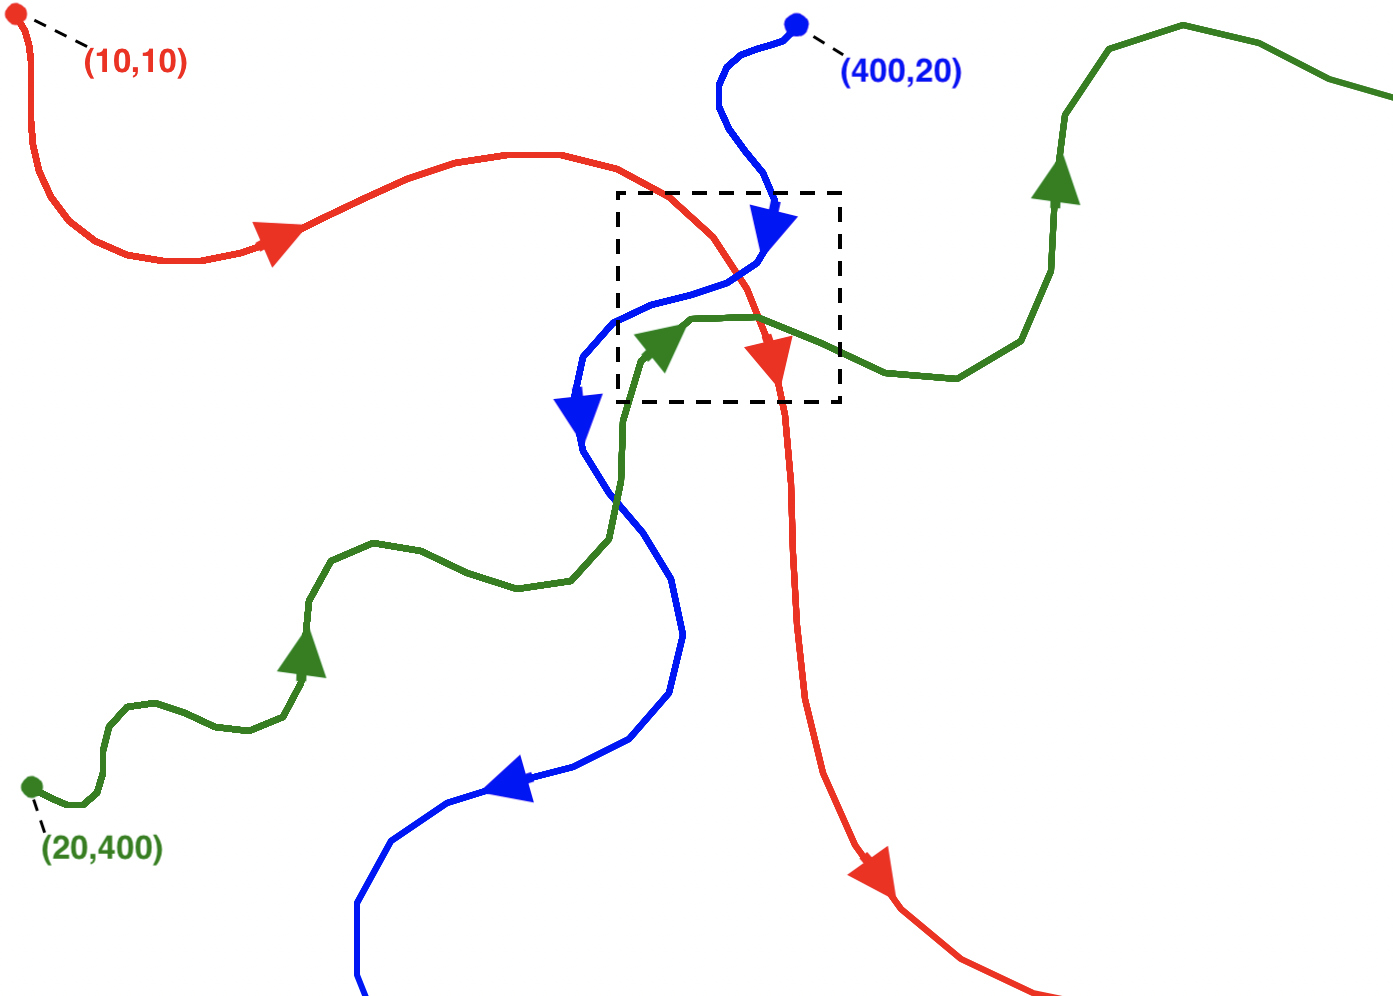
\includegraphics[width=0.75\textwidth]{images/curves.png}
    \caption{Synthetic curves with respective start positions}
    \label{fig:syntheticCurves}
\end{figure}

Generating rather complex curves instead of straight lines forces to agent to adjust its direction (and potential speed) at every timestamp. This is a test for an underlying policy to have a granular mapping from states to actions as well as the ability to recognize important (small) magnitudes of change in every state dimension. For example, we take the starting sequence of the green path generated by $curve_C$. In a small area which translate to a small range of x and y values, the agent has to perform rapid changes to the proposed direction in order to follow the sharp turns. Additionally, as the speed of the ground truth is constantly increases, the adjustment to the direction has to slow down for consecutive timesteps as the curves get stretched and have an increased amplitude.
\par
To add to the reasons of generating paths based on those three function, the positions and directions of the resulting trajectories challenge the agent to put special emphasis on a single feature dimension - the direction.  In order to understand why this is the case, we try to see the interaction cycle (recall subchapter \ref{chap:rlframework}) from the perspective of the agent. The agent is unaware of the history of positions (the trajectory) because it just receives the latest position with potentially more information such as speed and direction (depending on the variant of the environment). As indicated by the dashed rectangle in Fig. \ref{fig:syntheticCurves}, all three curves cross the same area. If for example the agent receives a state of $\{x=400, y=250\}$, it should perform an action which represents moving towards the bottom right if the ground truth trajectory is $curve_A$. However, the agent is unaware of the ground truth path or its type. Receiving the same or similar state in the next episode would result in the same action and choice of direction even though the internal ground truth trajectory change to $curve_B$ and actually requires the agent to move to the bottom left. The two synthetic paths $curve_B$ and $curve_C$ (green and blue) take this to the extreme as they move in near opposing directions. As a result, one hypothesis is that if the state representation is purely composed of the position (x and y coordinates), the agent is unable to differentiate between the three curves, as the states belonging to the different curves are not unique.
\par
Moreover, this is a test to whether or not it is even possible to learn representations of arbitrary paths which are not all part of single family of curves and can not be classified as the same type with minor variances.
Works like the one from \cite{martinsen2018curved} concentrate on special scenarios with almost identical paths to follow or split the split the dataset of AIS trajectories into groups of overall direction (e.g. moving from north to south or vice versa, leaving or entering the sea port, etc.) // cite edgardo?. Our desired goal is more comparable to the one presented by \cite{venskus2021unsupervised} who also try to predict vessel trajectories based on AIS data but without restricting or categorizing the tracks in a major way. The only factor that they use to split the tracks is the vessel type as they found out that different vessel types generate different traffic pattern thus they use one model per vessel type \cite[p.~729]{venskus2021unsupervised}.

// Markov property? history of states?
        \subsubsection{Variants}
        Being implemented in the programming language \textit{Python}, this environment implements the popular \textit{gym} interface "gym.Env" \cite[]{gym} for custom environments. This interface is de-facto standard when it comes to creating RL environments because all major RL and IL libraries (\textit{Stable-Baselines} \cite[]{stable-baselines3}, \textit{KerasRL} \cite[]{plappert2016kerasrl}, \textit{Acme} \cite[]{hoffman2020acme}, \textit{Spinning Up} \cite[]{SpinningUp2018}, etc.) implement their algorithms towards this interface.
\par
The interface itself requires the programmer to define an action- and observation space as attributes. In order to test which features have to be present in the observation space and how the agent reacts to a one or two dimensional action space, we define multiple variations of the environment. Besides the characterization of the action- and observation space, the interface includes a self explaining \textit{reset}-function and a \textit{step}-function which takes in an action as parameter and returns the next state, the reward, a boolean flag whether or not the terminal state is reached and optional information. Therefore, the \textit{step}-function represents the transition dynamics of the environment. We will try different approaches to the task of actually being able to predict future states of trajectories which in return is manifested in deviating transition dynamics and \textit{step}-function thus resulting in another set of variants.

\paragraph{States and actions.} Choosing the right state representation is mandatory for the agent to take the correct actions. In this case, the MDP framework assumes that the state representation fulfills the \textit{Markov} property which implies that a single state in the present (no history involved) retains all relevant information for the agent to distinguish between different environment setups to be able to make suitable decisions. We will intentionally break this assumption by constructing one variant that has a state representation of just $\{x,y\}$ to the importance of the \textit{Markov} property.
\par
To make different trajectories distinguishable by the state representation, the direction has to be added as well. For the simply case, we want the agent to solely select its direction at each timestep and let the environment specify the perfect speed value. A more demanding variant adds the speed component to the state representation and the action space, making them four and two dimensional.
\par
The analysis and discussion about the results will show that even a state representation of position, speed and direction might not fulfill the assumption of a markovian state. Hence, we will also try state representations that include the current distance to the ground-truth (GT) as well as a representation that contains the current timestep. Incorporating a time component into the state model was already mentioned in the related work section of this thesis (see chapter \ref{chap:relatedWork}) in context of the work proposed by \cite{liu2019vessel} who include a Unix timestamp to their state representation.

\begin{equation}
\begin{aligned}
    S1 := S_t &= \{x_t,y_t\}
\\
    S2 := S_t &= \{x_t,y_t, direction_t\}
\\
    S3 := S_t &= \{x_t,y_t, direction_t, speed_t\}
\\
    S4 := S_t &= \{x_t,y_t, direction_t, speed_t, distance_t\}
\\
    S5 := S_t &= \{x_t,y_t, direction_t, speed_t, t\}
    \end{aligned}
\end{equation}\label{stateRepresentation}

For clarity, we defined the labels for the action features as "course" and "tempo" to better indicate that they are independent from the "direction" and "speed" features of the state representation.
\begin{equation}
\begin{aligned}
    A1 := A_t &= \{course_t\}
\\
    A2 := A_t &= \{course_t, tempo_t\}
    \end{aligned}
\end{equation}

\paragraph{Transition dynamics.} The core of every environment are its transition dynamics. Normally, the respective \textit{step}-function is well defined and meant to be immutable. Meaning, that the environment dynamics are set before the application of any RL algorithms and those algorithms actually try to solve the sequential decision problem that arises by the interaction with the environment. In our case, we try to squeeze the task of predicting future vessel trajectories into the RL framework trying to approach the task in a different way by making an agent interact and select at every timestep instead of for example looking at the problem as a timeseries prediction exercise. Hence, we are in charge of constructing artificial transition dynamics that best fit to our problem. It is even imaginable and most likely unavoidable that an agent trains in one environment but uses its learned policy in another environment with different transition dynamics that depict the real-world use case. This is due to the fact that training has to include some sort of guiding historical ground-truth trajectories which are not present in the actually application of predicting paths.
\par
While looking at the overall task again, we construct a set of different transition dynamics. The ground-truth data consists of starting points and functions that generate direction values at every timestep. We call this instance GT for ground truth which shares the same concept as the agent. The GT and the agent both have a current position which in conjunction with the proposed direction is used to calculate the next position. The histories of positions which are unknown to the agent are the ground truth trajectory and the generated trajectory by the agent. If we ignore the speed component for this explanation, the agent receives an initial state $\{x_0,y_0,heading_0\}$ which is identical to the GT. Next, the agent selects a value for the direction it should move ($a_0=\{direction_0\}$). Internally, the next GT position is calculated by using its current x,y coordinates at $t=0$ and the output of the curve-function for $t=1$. The next agent position is derived from ($x_0, y_0$) and the proposed direction from the action. For both calculations an internal value for the current speed is utilized. The next state consists of the agent's current x and y values and the current heading which in fact is the same as the previously proposed direction. Consequently, the agent tries to predict the next output value of the underlying curve function at $t+1$ to move in the same direction as the GT in order to stay as close as possible to the current GT position.
\par
Our assumption is that after the training phase, the agent successfully learned to map $\{x_0,y_0,heading_0\}$ states to the corresponding GT direction values of the future next state. This policy is then used in a customized version of the environment which does not include GT data but uses the same routine to calculate next points given the current agent position and the suggested direction. In other words, the agent's policy is trained by learning the same underlying policy of the GT in order to generate representative trajectories.
\par
Passing through the journey of creating multiple experiments and different approaches, we also take a deviating route to the one mentioned in the previous paragraph. Instead of returning the agent's next position and heading, the \textit{step}-method will return the next state of the GT. At first this may sound contradictory to what we discussed regarding the RL framework because the agent does not fully experience the potential drawbacks of past decisions. Even if the agent selects an action which leads to the agent drifting heavily apart from the GT, the next state will still be an optimal state of the GT. The reason behind this approach is the idea, that the agent learns the desired mapping more efficiently since suboptimal decisions do not accumulate error and provoke bad states which the agent is unable to recover from. As a matter of fact, the mechanism of recovery, meaning that the state space is expanded by e.g. a feature that tells the agent how far away it is from the GT and in what direction, is impossible as a consequence of the missing GT in the real-world scenario. The major speculation that is up for testing is the possible transfer of the trained policy which - in the training phase - receives next states from the GT, to a production environment without GT and adjusted transition dynamics that return states purely based on the agent's kinematics (except for the initial state).
        \subsubsection{Reward Function}\label{subchap:reward}
        The desired goal we want the agent to achieve is to stay as close as possible to the GT positions in order to generate identical paths. A reward function should consequently assign positive feedback if the agent is near the GT. Punishing the agent with negative rewards if it drifts apart from the GT is not practical because initial experiments show that the agent will just move straight out of bounds to end the episode. Any RL algorithm tries to maximize the return. If the agent continuous to explore the state space, it will repeatedly receive negative rewards which accumulate to a high negative return. However, moving straight out of bounds will result in a return of a few negative rewards which is greater than any attempt to follow the curve. Accordingly, we will use the Gaussian track-error, mentioned in the work of \cite{martinsen2018curved}, as inspiration to construct the reward function. Rewards are exclusively positive, starting at 1 if the positions are the same, and get smaller in proportion to the current distance between the agent's position and the GT's position. \cite{martinsen2018curved} use a normal distribution to determine the scalar reward based on the distance (p.~X). At the beginning of our modelling and experiment phase, we make use of a customized version of such a normal distribution as reward function as well. Besides, we come up with another reward function which is based on a rectified linear function. The idea being that the non-linearity of the Gaussian distribution distorts the evaluation metrics as the average reward can not be interpreted as mean distance. 
\par
Additionally a reward signal is built that includes past feedback and can be seen as moving sum or moving average of the prior described reward functions. This reward function is inspired by the work of \cite{edgarod} who set up a reward signal that //todo.


\begin{figure}[H]
    \centering
    \begin{subfigure}[b]{0.495\textwidth}
        \includesvg[width=\textwidth]{images/r1.svg}
        \label{fig:reward1}
    \end{subfigure}
    \begin{subfigure}[b]{0.495\textwidth}
        \includesvg[width=\textwidth]{images/r2.svg}
        \label{fig:reward2}
    \end{subfigure}
    \caption{Different reward functions that map distances between agent and GT positions in pixels to scalar reward values. (a) Gaussian track error. (b) Rectified linear reward function}
    \label{fig:rewardFunctions}
\end{figure}

\begin{equation}
\begin{aligned}
    R1 := f_{R1}(d_t) &= \frac{1}{5 \sqrt{2\pi}} \mathrm{e}^{-\frac{d_t^2}{50}} \cdot 12.5333
\\
R2 := f_{R2}(d_t) &= max(1 - \frac{d_t}{10}, 0)
\\
    R3 := f_{R3}(d_t) &= \sum_{i=0}^{10}{f_{R1}(d_{t-i})}
\\
    R4 := f_{R4}(d_t) &= \frac{f_{R3}(d_t)}{10}
    \end{aligned}
\end{equation}

        
    \subsection{Performance Metric}
    In order to evaluate the performance across different experiment setups that include different reward functions, a unified and comparable metric has to be defined. Again, because the reward functions are up to test and will be switched out during separate runs, as well as the fact that the episodes do not have the same lengths, analyzing based on the collected cumulative reward is not practical. Additionally, when applying behavioral cloning in subchapter \ref{subchap:applyBC}, there is no reward function involved, showing the need for a metric that can also be used to compare different methods.
\par
Since we do want the agent to follow the GT position as close as possible, we use the average \textit{Euclidean distance} between the proposed paths by the agent and the GT as a performance metric throughout the synthetic and the real-world experiments. In this regard, we will use the word "performance" as synonym for the average euclidean distance.
\par
The performance $p$ of the agent during an episode of $N$ time steps can thus be calculated as:
\begin{equation}
    p = \frac{1}{N} \sum_{t=0}^{N}\sqrt{(x^{agent}_i - x^{GT}_i)^2 + (y^{agent}_i - y^{GT}_i)^2}
    \label{eq:euclid}
\end{equation}


    \subsection{Applying DDPG}
    We conducted over 20 experimental setups, with each one consisting of five independent runs with different seeds. In this chapter, a subset of the results is displayed and the systematic approach of finding suitable hyperparameters and the interpretation about their influence is described. A table of all results can be found in the appendix in section \ref{appendix:curveResults}.
\par
Let us start by recalling what components are present and whether they are immutable during our experiments. Foremost, there are five different state representations and their corresponding action spaces as the simplest environment in the case of $S1$ and $S2$ adjusts the speed automatically. The combinations to test are thus $S1\_A1$, $S2\_A1$, $S3\_A2$, $S4\_A2$ and $S5\_A2$.
\par
Next are the hyperparameters as described in \ref{subchap:hyperparameters}. We will keep the values of the parameters unchanged during the experiments except for the replay buffer size and $\sigma$, which has a huge influence on the exploration due to its impact on the noise process (see Fig. \ref{fig:ouProcess}). We adjust the source code of the Stable-Baselines3 library to support different learning rates for the actor and critic networks to stay in line with the theoretical findings of chapter \ref{subchap:hyperparameters}. Hence, we use a fixed learning rate of $10^{-4}$ for the actor and  $10^{-3}$ for the critic. The training lasts for a fixed duration of 30,000 time steps, which translates to almost identical numbers of network updates (during the initial filling of the replay buffer no updates are done) and 492 episodes. We described the neuronal network architecture by using the notion $n_h^i= N$, where $n$ is the $i$-th hidden layers, starting at 1, with $N$ neurons. The hyperparameters are summarized as follows:

\begin{table}[H]
\centering
\begin{tabular}{|l|l|}
\hline
\textbf{Name}                & \textbf{Value}                                                \\ \hline
Training Steps               & $30.000$                                                      \\ \hline
Network Architecture         & $n_{h}^{1}=400$ and $n_{h}^{2}=300$       \\ \hline
Learning Rates               & $\alpha_{actor} = 10^{-4}$ and $\alpha_{critic}= 10^{-3}$     \\ \hline
Batch Size                   & $128$                                                         \\ \hline
Soft Update Parameter $\tau$ & $10^{-3}$                                                     \\ \hline
Discount Factor $\gamma$     & $0.99$                                                        \\ \hline
Replay Buffer Size           & $5\cdot 10^4$ or $5 \cdot 10^6$                               \\ \hline
Noise Parameter              & $\mu=0$, $\theta=0.15$, $\sigma$ is $0.05$ or $0.15$ or $0.5$ \\ \hline
\end{tabular}
\caption{\label{tab:hyperDDPG} Hyperparameter setup during DDPG training of the synthetic experiments}
\end{table}
\par
Lastly, investigations are done on the effect of the three different reward function ($R1$, $R2$ and $R3$) as defined in subchapter \ref{subchap:reward}.
\par
As a starting point, we interpret the results of the first sets of experiments, conducted with $\sigma=0.05$ and a replay buffer size of $N=5 \cdot 10^4$. A small value of $\sigma$ translates to overall smaller amplitudes in the Ornstein-Uhlenbeck process, which causes the noise to be added to suggested actions to alternate between $-0.5$ and $0.5$ as illustrated in Fig. \ref{fig:lowSigmaNoise}. The intention behind a low $\sigma$ value is related to the small replay buffer size because we do not want to fill up the buffer majorly with extreme action values close to or clipped at $-1$ and $1$. The upcoming table shows the performances (euclidean distances) and standard deviations of the best-seed runs and the respective euclidean distances of the agent's suggested and the ground-truth curves.

% Please add the following required packages to your document preamble:
% \usepackage[table,xcdraw]{xcolor}
% If you use beamer only pass "xcolor=table" option, i.e. \documentclass[xcolor=table]{beamer}
\begin{table}[H]
\centering
\begin{tabular}{|l|l|l|l|l|}
\hline
\multicolumn{1}{|c|}{\textbf{Experiment}} & \multicolumn{1}{c|}{\textbf{Overall Performance}} & \multicolumn{1}{c|}{\textbf{Curve\_A}} & \multicolumn{1}{c|}{\textbf{Curve\_B}} & \multicolumn{1}{c|}{\textbf{Curve\_C}} \\ \hline
$S1\_A1\_R1$                              & $207 \pm 180$                                     & $183$                                  & $319$                                  & $141$                                  \\ \hline
$S1\_A1\_R3$                              & $134 \pm 149$                                     & $130$                                  & $198$                                  & $87$                                   \\ \hline
$S2\_A1\_R1$                              & $141 \pm 122$                                     & $180$                                  & $156$                                  & $91$                                   \\ \hline
$S2\_A1\_R3$                              & $132 \pm 148$                                     & $112$                                  & $194$                                  & $101$                                  \\ \hline
$S3\_A2\_R1$                              & $165 \pm 158$                                     & $117$                                  & $312$                                  & $93$                                   \\ \hline
$S3\_A2\_R2$                              & $173 \pm 127$                                     & $195$                                  & $211$                                  & $121$                                  \\ \hline
$S3\_A2\_R3$                              & $154 \pm 116$                                     & $144$                                  & $116$                                  & $195$                                  \\ \hline
$S4\_A2\_R1$                              & $112 \pm 123$                                     & $117$                                  & $87$                                   & $128$                                  \\ \hline
{\color[HTML]{333333} $S4\_A2\_R2$}       & {\color[HTML]{333333} $91 \pm 98$}                & {\color[HTML]{333333} $56$}            & {\color[HTML]{333333} $134$}           & {\color[HTML]{333333} $90$}            \\ \hline
$S4\_A2\_R3$                              & $80 \pm 88$                                     & $71$                                  & $49$                                  & $112$                                  \\ \hline
$S5\_A2\_R1$                              & $199 \pm 118$                                     & $195$                                  & $204$                                  & $197$                                  \\ \hline
$S5\_A2\_R2$                              & $219 \pm 115$                                     & $238$                                  & $238$                                  & $185$                                  \\ \hline
\end{tabular}
\caption{ Performances of several experiments with $\sigma = 0.05$ and replay buffer size of $N=5 \cdot 10^4$.}
\label{tab:resultsK3}
\end{table}

To understand what these numbers really mean, we have to dive into deeper analysis and have to visualize actual trajectories produced by the agent. We first concentrate on the simplest environment variant, which does not require the agent to choose a speed value ($S1\_A1$ and $S2\_A1$). One assumption is that the state representation of $S1$ is insufficient due to the fact that the agent has no way to identify unique states of different curves if only $x$ and $y$ are given. However, the performances of $S1\_A1\_R3$ and $S2\_A2\_R3$ are almost identical. The question arises if this proves that the assumption is wrong or the agent fails the task catastrophically in both cases? To answer this question, we visualize both runs in a way to quantify the evolving distances during each of the three different episodes:
\par

\begin{figure}[H]
     \centering
     \begin{subfigure}[b]{0.9\textwidth}
         \centering
         \includesvg[width=\textwidth]{images/ddpg_results/simple_envs_S1_S2/ddpg_S1_A1_R3_K3.svg}
         \caption{$S1\_A1\_R3$}
     \end{subfigure}
\end{figure}
\begin{figure}[H]\ContinuedFloat
     \begin{subfigure}[b]{0.9\textwidth}
         \centering
         \includesvg[width=\textwidth]{images/ddpg_results/simple_envs_S1_S2/ddpg_S2_A1_R3_K3.svg}
         \caption{$S2\_A1\_R3$}
     \end{subfigure}
        \caption{Distances between the path proposed by the agent and the GT over time. $\sigma = 0.15$ and $N=5\cdot 10^4$.}
        \label{fig:simpleCurves1}
\end{figure}

Fig. \ref{fig:simpleCurves1} displays the inability of both state representations to follow and reproduce $curve\_B$ as both setups drift apart from the GT right at the beginning, reaching a distance from over 200 just 20 time steps into the episode. However, we do see similar mediocre performances in terms of the $curve\_A$ and $curve\_B$, with $S2$ following $curve\_A$ exceptional well in the mid-part of the episode between time steps 15 to 23. To analyze the behavior of the agent on an empirical level, we also visualize the generated trajectories by the agent. Please note, that the performance metric includes a  time component and the portrayal of the paths could lead to misinterpretation, for example, if the agent follows the path perfectly but on a slower pace. Nevertheless, those illustrations greatly help to analyze the behavior of the agent and algorithm. 

\begin{figure}[H]
     \centering
     \begin{subfigure}[b]{0.31\textwidth}
         \centering
         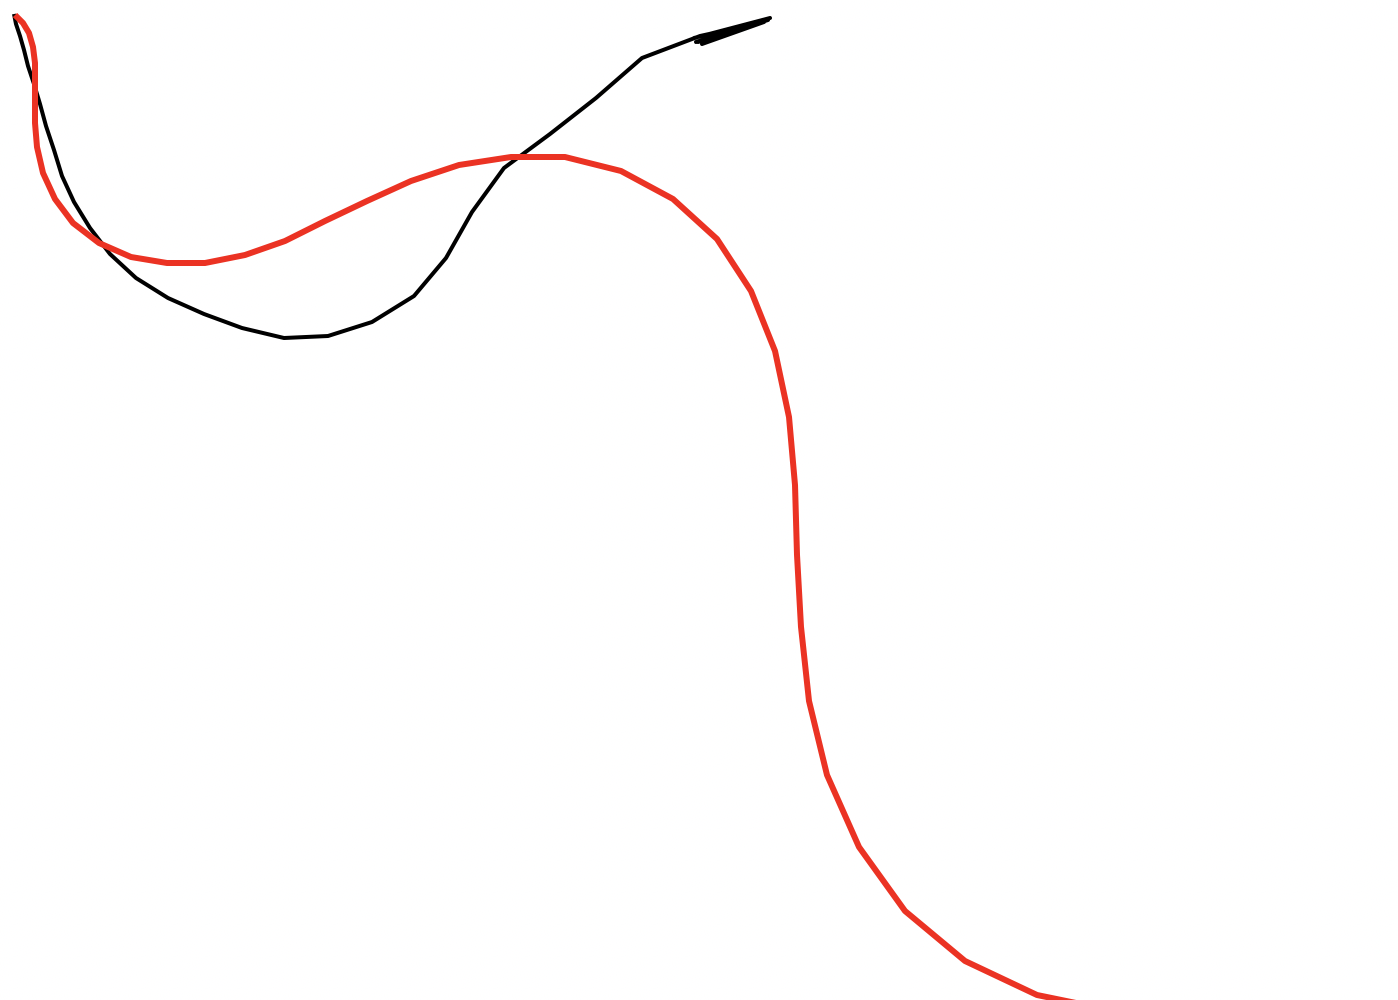
\includegraphics[width=\textwidth]{images/ddpg_results/simple_envs_S1_S2/S1_A1_R3_K3_curve_A.png}
         \caption{$curve\_A$}
     \end{subfigure}
     \hfill
     \begin{subfigure}[b]{0.31\textwidth}
         \centering
         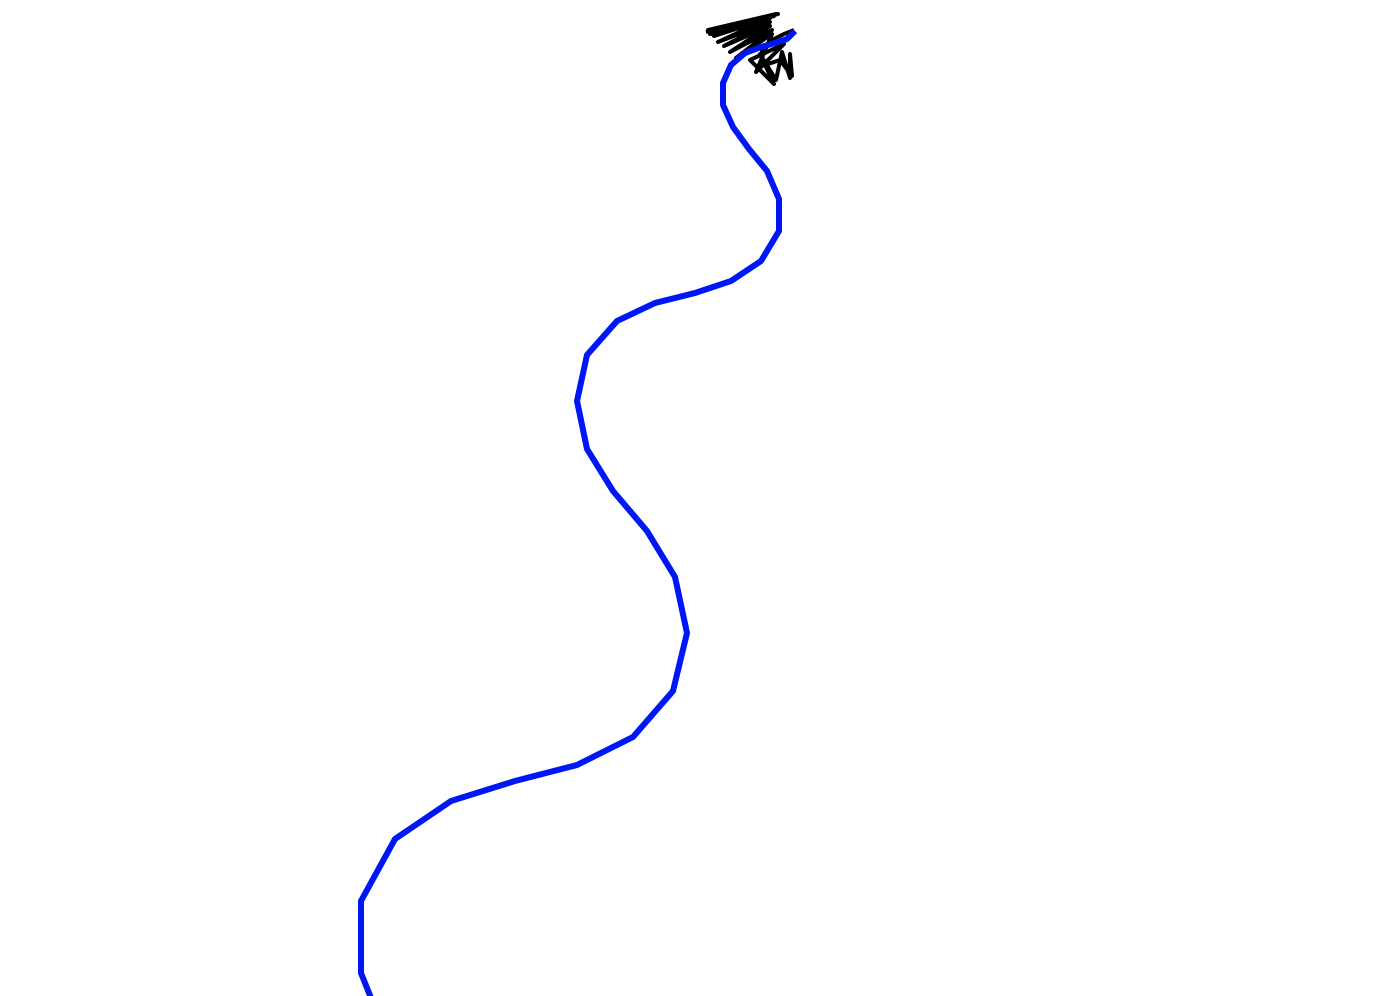
\includegraphics[width=\textwidth]{images/ddpg_results/simple_envs_S1_S2/S1_A1_R3_K3_curve_B.png}
         \caption{$curve\_B$}
     \end{subfigure}
     \hfill
     \begin{subfigure}[b]{0.31\textwidth}
         \centering
         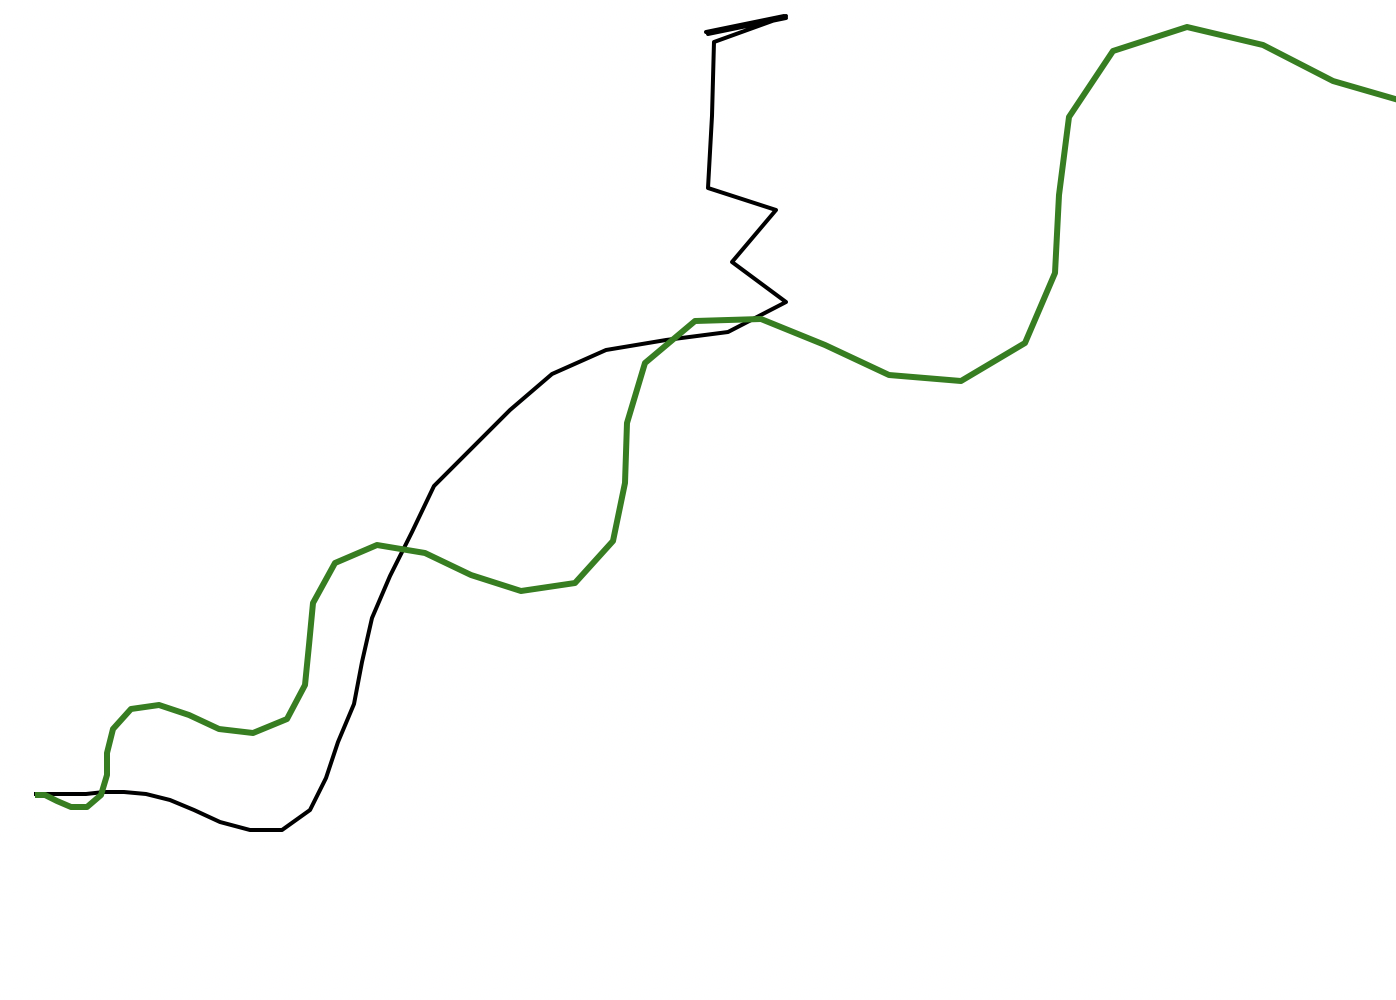
\includegraphics[width=\textwidth]{images/ddpg_results/simple_envs_S1_S2/S1_A1_R3_K3_curve_C.png}
         \caption{$curve\_C$}
     \end{subfigure}
        \caption{$S1\_A1\_R3$}
        \label{fig:simpleCurves2}
\end{figure}



\begin{figure}[H]
     \centering
     \begin{subfigure}[b]{0.31\textwidth}
         \centering
         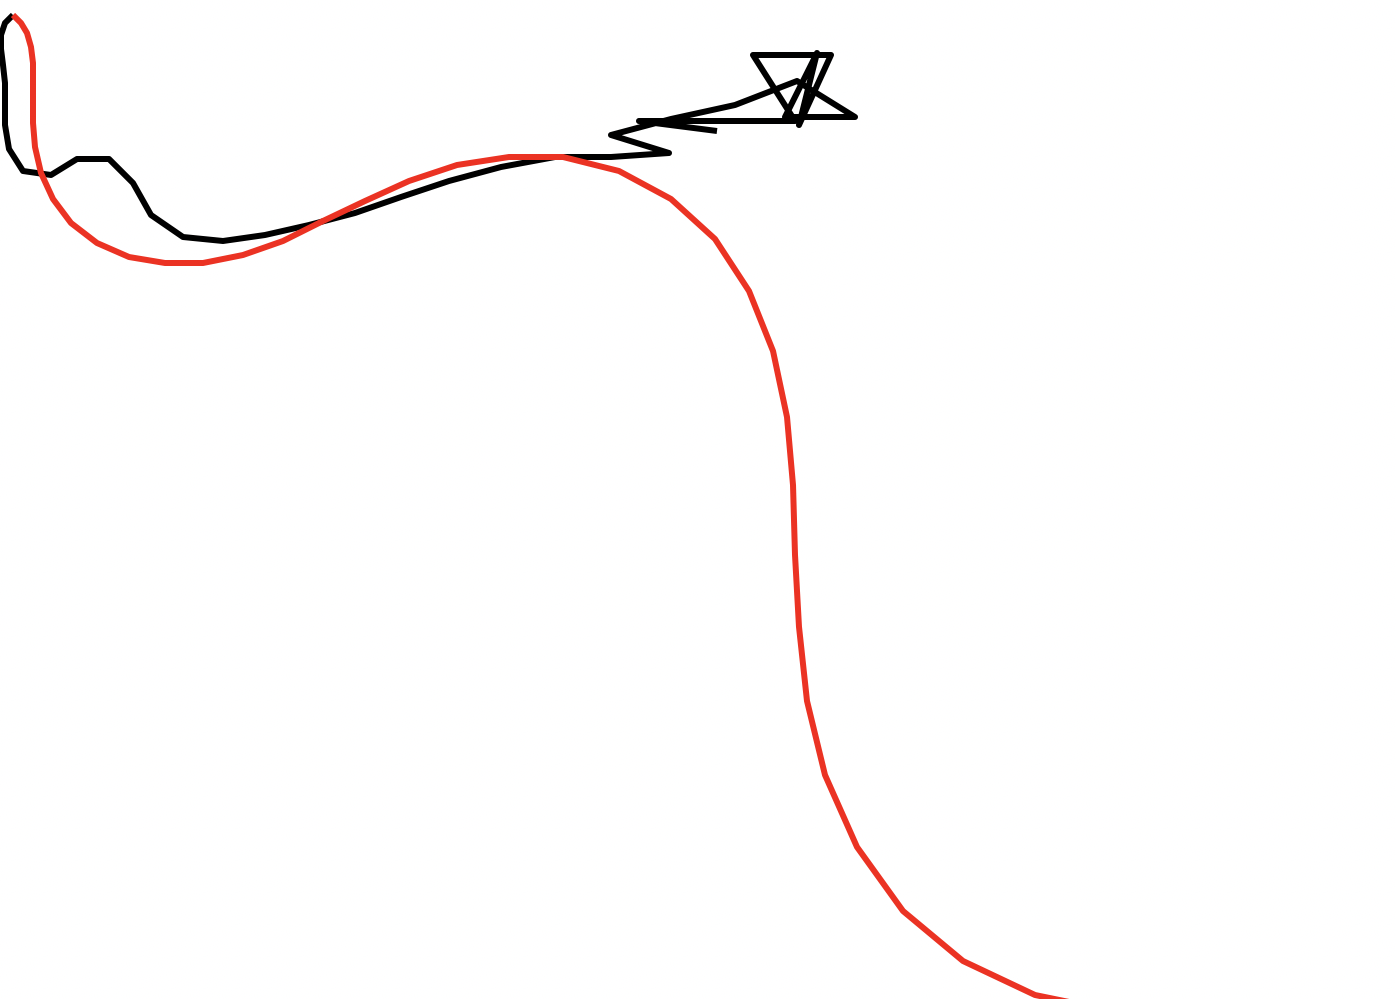
\includegraphics[width=\textwidth]{images/ddpg_results/simple_envs_S1_S2/S2_A1_R3_K3_curve_A.png}
         \caption{$curve\_A$}
     \end{subfigure}
     \hfill
     \begin{subfigure}[b]{0.31\textwidth}
         \centering
         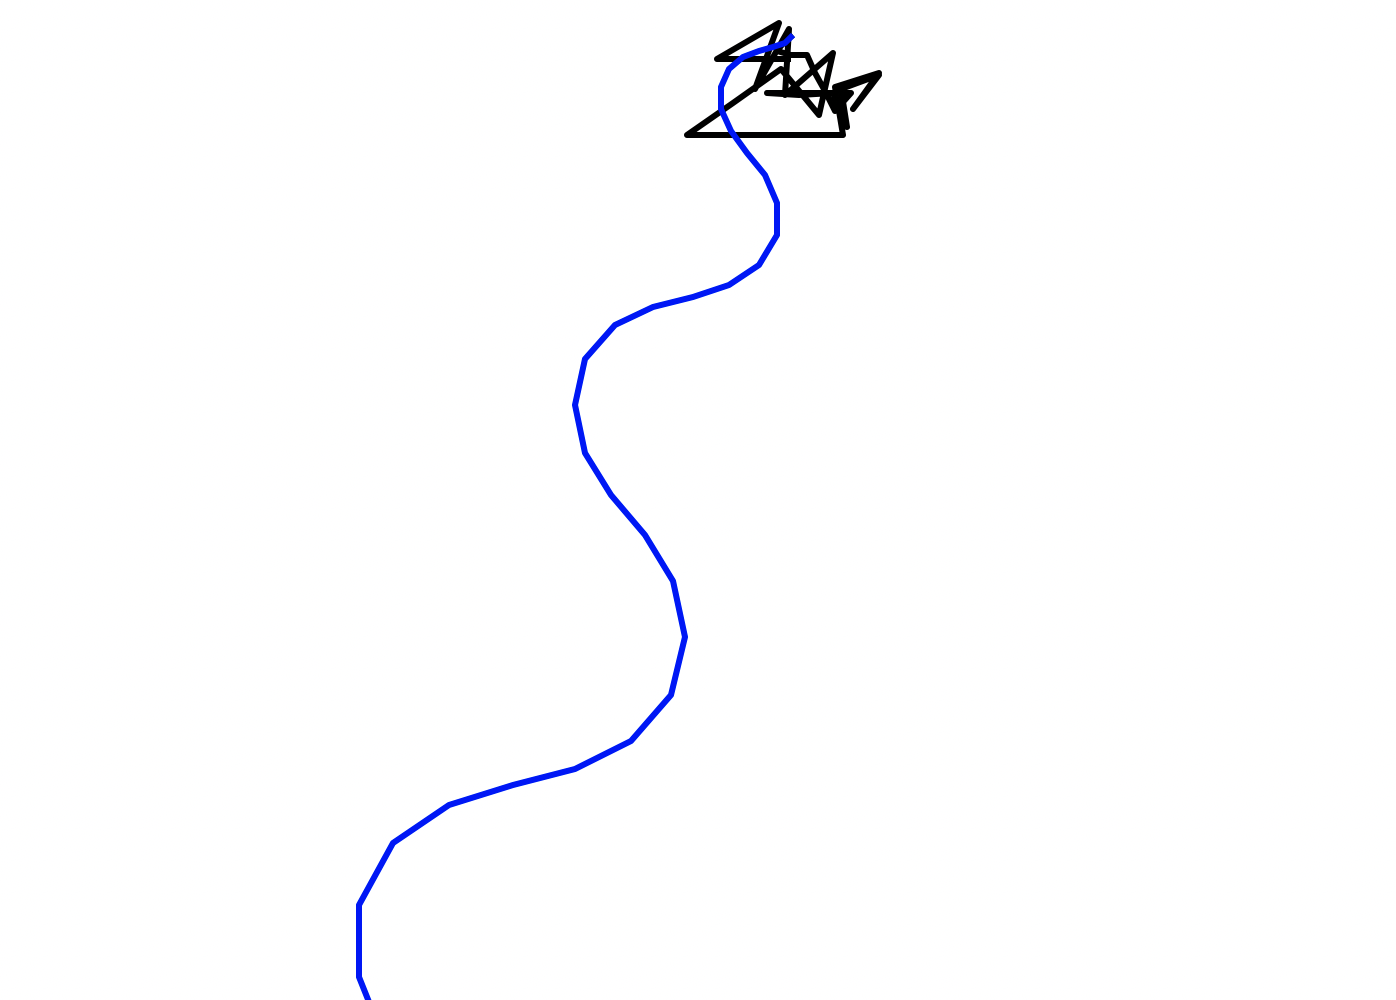
\includegraphics[width=\textwidth]{images/ddpg_results/simple_envs_S1_S2/S2_A1_R3_K3_curve_B.png}
         \caption{$curve\_B$}
     \end{subfigure}
     \hfill
     \begin{subfigure}[b]{0.31\textwidth}
         \centering
         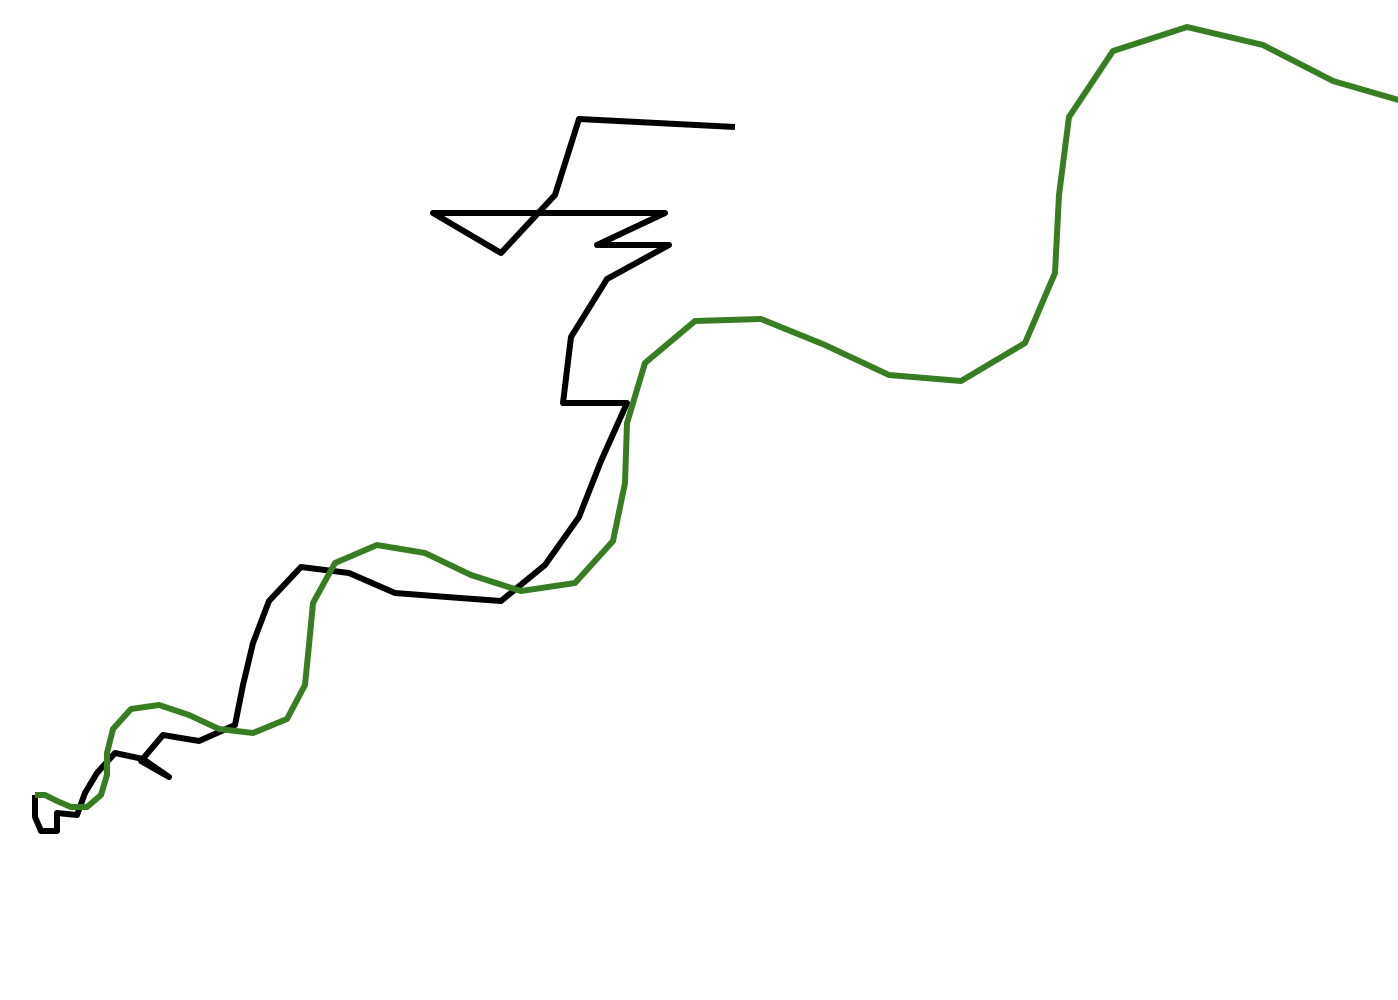
\includegraphics[width=\textwidth]{images/ddpg_results/simple_envs_S1_S2/S2_A1_R3_K3_curve_C.png}
         \caption{$curve\_C$}
     \end{subfigure}
        \caption{$S2\_A1\_R3$}
        \label{fig:simpleCurves3}
\end{figure}

The illustrations of Fig. \ref{fig:simpleCurves2} and \ref{fig:simpleCurves3} indeed reveal catastrophic failure to the task for both state representations. Although the starting time steps for $curve\_A$ and $curve\_C$ look promising, the agent suddenly drifts apart heavily from the GT path. It is noticeable that the agent, in all cases, moves towards a certain area to then start fluctuating the proposed heading value so much that it stays in the area. The area is located in the center top of the map where the blue $curve\_B$ has its starting position, which in returns explains the bad performance for this specific curve. 
\par
It is hard to reason exactly what is causing this behavior. One reason could be the $\sigma$ value being too low so that the agent is unable to explore the correct heading values for $curve\_B$, which eventually leads to randomly guessing values right at the beginning of the episode of $curve\_B$ and thus the filling of the replay buffer with bad transition tuples. Another possible explanation for this behavior could be that the replay buffer is too small, only fitting in $5\cdot 10^4$ transitions. Another indicator of this could be the general drift after approximately 25 time steps for $curve\_A$ and $curve\_C$ as the replay buffer is unable to contain the transition tuples for the complete paths.
\par
To test these hypotheses, we conduct another set of experiments with an increased value for $\sigma$ and a replay buffer size of $N=5\cdot 10^6$. The performances are $157 \pm 145$ in the case of $S1\_A1\_R3$ and $182 \pm 181$ for $S2\_A1\_R3$ which is even worse than the results of the previous setting display in Tab. \ref{tab:resultsK3}. The generated paths of the best run of $S2\_A1\_R3$ show that the agent now starts fluctuating on place for $curve\_C$ as well:

\begin{figure}[H]
     \centering
     \begin{subfigure}[b]{0.31\textwidth}
         \centering
         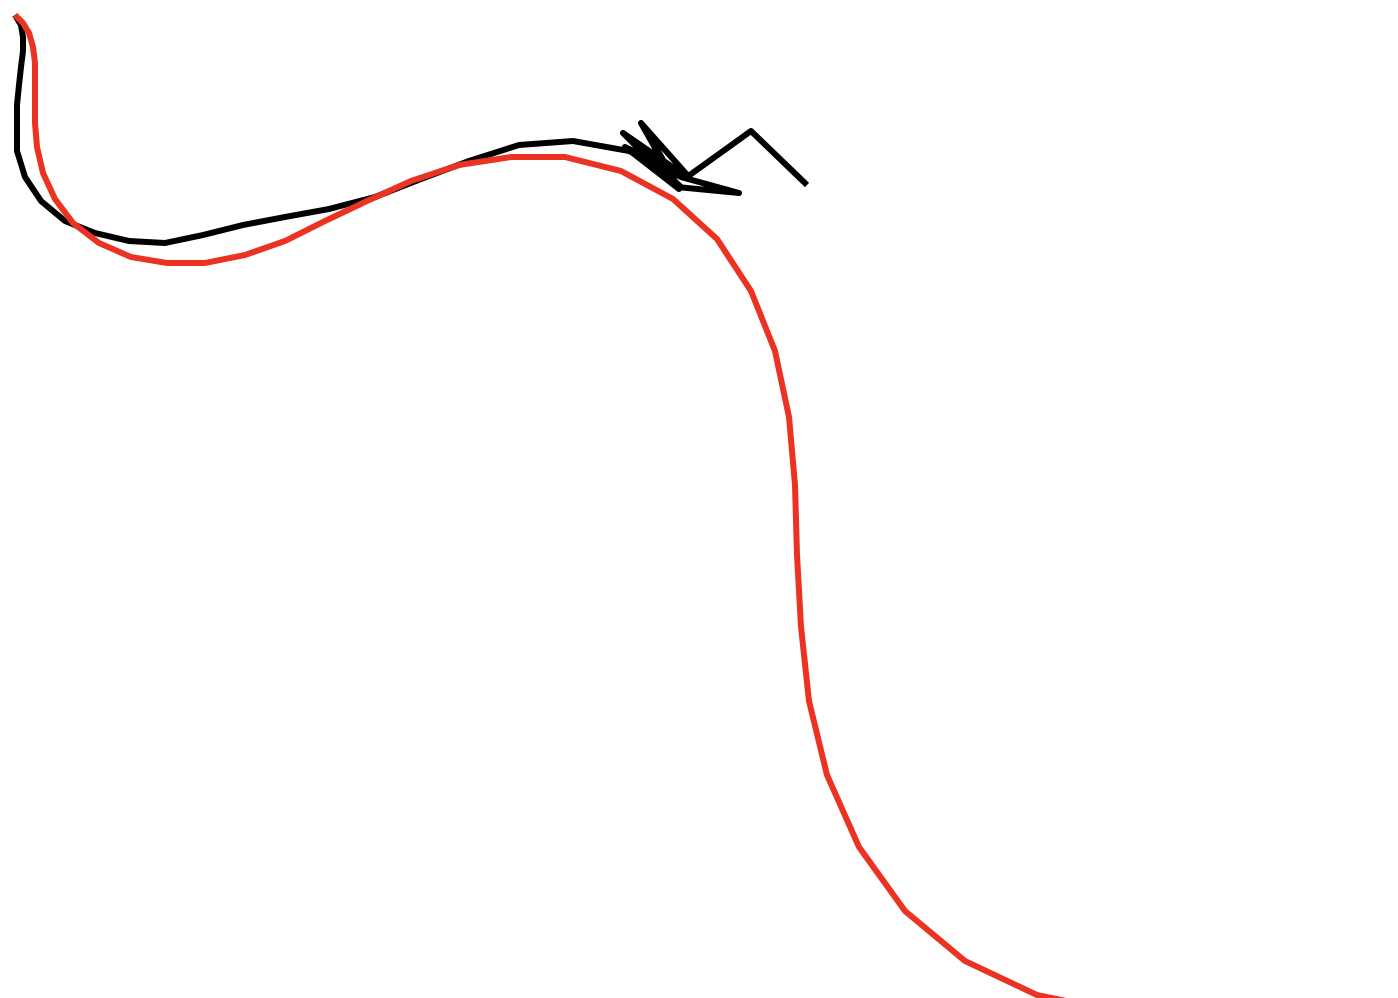
\includegraphics[width=\textwidth]{images/ddpg_results/simple_envs_S1_S2/S2_A1_R3_5mio_curve_A.png}
         \caption{$curve\_A$}
     \end{subfigure}
     \hfill
     \begin{subfigure}[b]{0.31\textwidth}
         \centering
         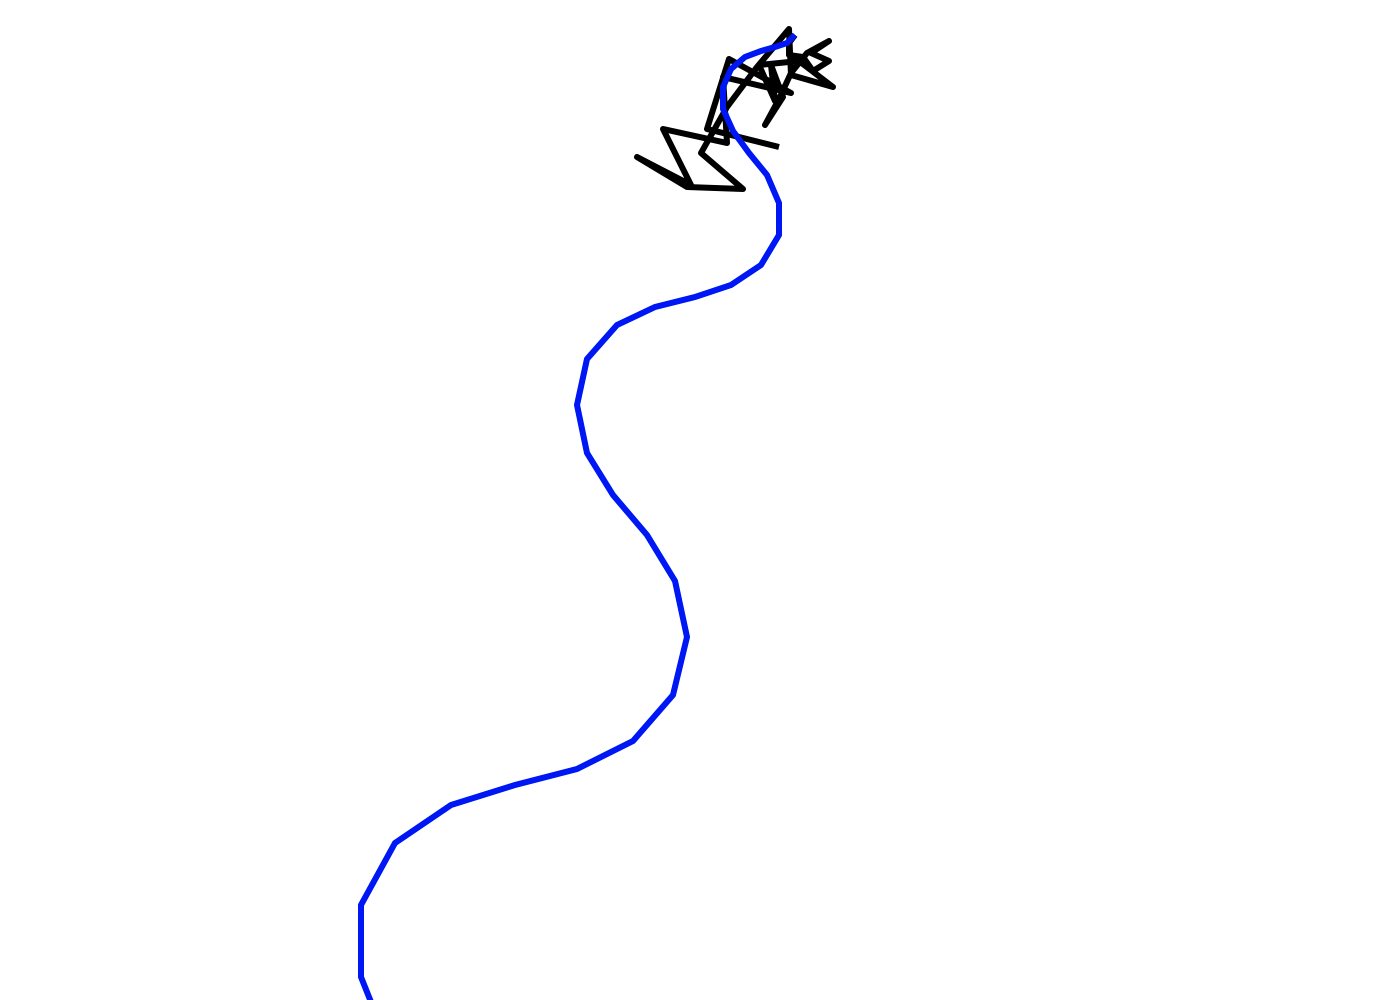
\includegraphics[width=\textwidth]{images/ddpg_results/simple_envs_S1_S2/S2_A1_R3_5mio_curve_B.png}
         \caption{$curve\_B$}
     \end{subfigure}
     \hfill
     \begin{subfigure}[b]{0.31\textwidth}
         \centering
         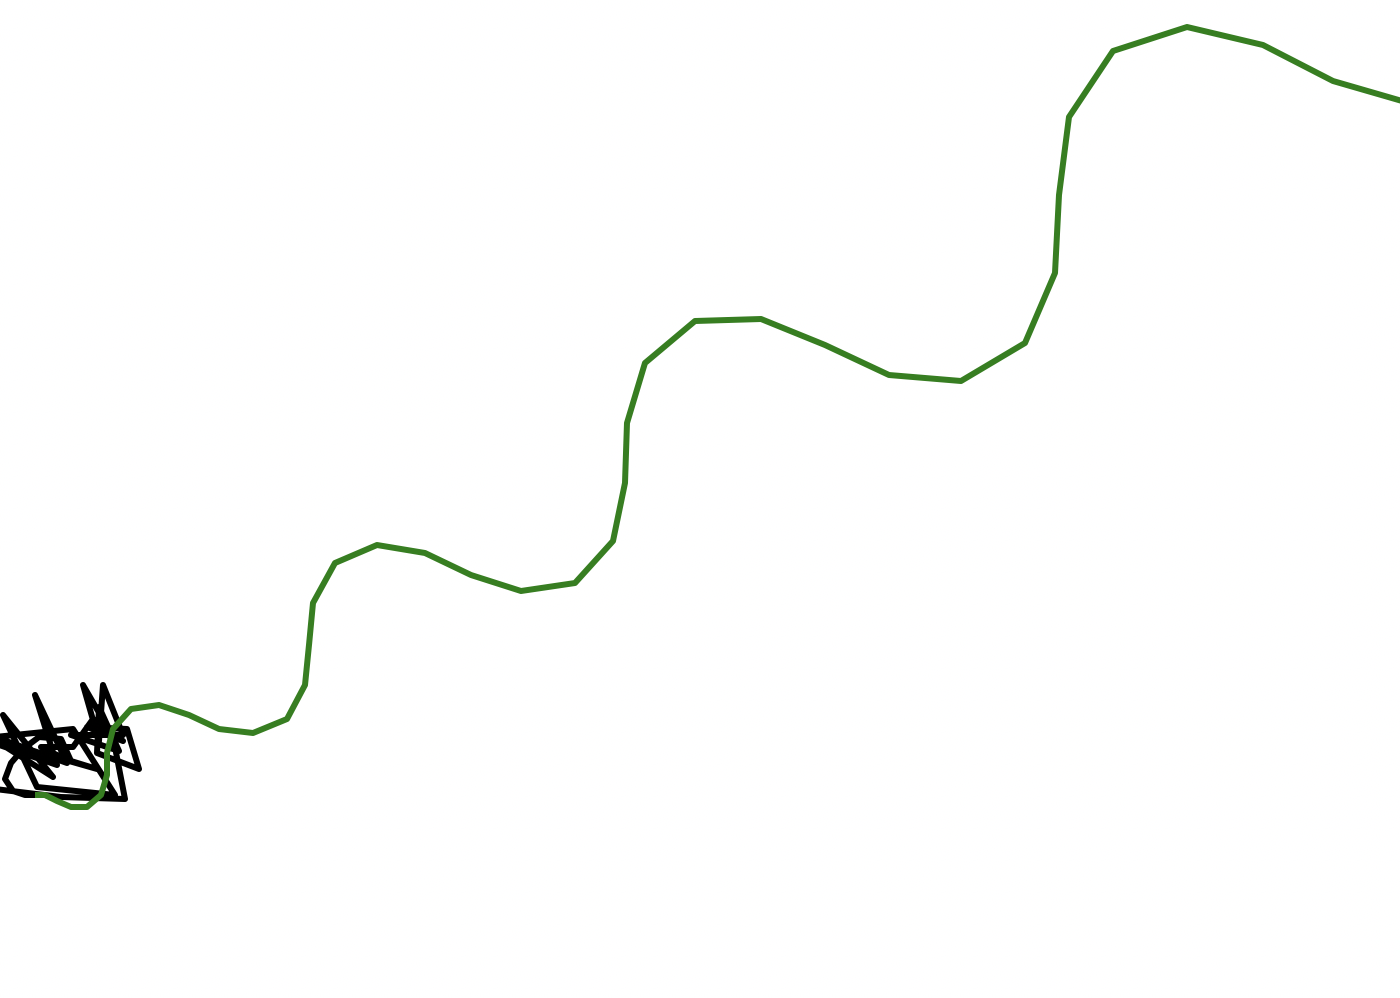
\includegraphics[width=\textwidth]{images/ddpg_results/simple_envs_S1_S2/S2_A1_R3_5mio_curve_C.png}
         \caption{$curve\_C$}
     \end{subfigure}
        \caption{$2\_A1\_R3$ using $\sigma=0.15$ and a replay buffer size of $N=5\cdot 10^6$.}
        \label{fig:simpleCurves4}
\end{figure}

Due to the fact that the agent starts following the $curve\_A$ as intended, we rule out a bug in our implementation of the environment or the transition dynamics. Additionally, the second experiment shows that extending the replay buffer size has not a positive impact for this supposedly simple task in terms of episode lengths. We do conclude that the reason for failure is situated in the reward function or in the state representation which causes the environment to not be "Markov enough".
\par
It should be noted that the experimental setups of $S1$ and $S2$ do not represent the actual task, as they drop the requirement for the agent to adjust the speed. Although those presumably easier setups fail, we still investigate the setups of two-dimensional action spaces including the speed, but also testing additional features for the state representation. In the previous paragraph we wrote not "Markov enough". What we mean by this is the fact that the agent is unable to distinguish between states that, e.g., have the same values $\{x, y, heading\}$ but occur on different time steps. The agent start jumping back and forth endlessly because the policy is a deterministic mapping of states to actions. In the end, it is the goal of the agent to learn a policy that perfectly maps states to actions to generate the exact trajectories. Though, the learning process when using DDPG might not be suitable to actually get to a mapping like this if the state representation does not fully represent the environment at a certain time step, e.g., missing a time component or the position of the GT.
\par
Aiming to test our assumptions, we construct three different state representations. Equation \ref{stateRepresentation} suggests that $S3$ is a nomenclature for the environment states, defined by \linebreak $\{x, y, heading, speed\}$. Additionally, we come up with $S5$ which  adds the current time step of the episode to the state, a technique also used by \cite{liu2019vessel} and discussed in chapter \ref{chap:relatedWork}. Finally, we also construct $S4$ as a possible state representation which adds the current distance between the agent's position and the GT position. However, it is important to note that this state representation just serves as theoretical experiment because it is not possible to apply it to the real-world scenario, as the GT is not present when predicting paths.
\par
Despite the assumption that adding the current time step as a feature should make the states more distinguishable, the performances of experiments conducted with $S5$ do not outperform those of $S3$. During the search for the best hyperparameters, the euclidean distances vary from 126 up to 252 for $S5$ and 136 to 194 in the case of $S3$. A value of $\sigma = 0.15$ and a small replay buffer size of $N=5 \cdot 10^4$ yield the best results for $S3$ as well as $S5$. 
\begin{figure}[H]
     \centering
     \begin{subfigure}[b]{0.9\textwidth}
         \centering
         \includesvg[width=\textwidth]{images/ddpg_results/envs_S3_S4_S5/ddpg_S3_A2_R3.svg}
         \caption{$S1\_A1\_R3$}
     \end{subfigure}
\end{figure}
\begin{figure}[H]\ContinuedFloat
     \begin{subfigure}[b]{0.9\textwidth}
         \centering
         \includesvg[width=\textwidth]{images/ddpg_results/envs_S3_S4_S5/ddpg_S5_A2_R3.svg}
         \caption{$S2\_A1\_R3$}
     \end{subfigure}
        \caption{Distances between the path proposed by the agent and the GT over time. $\sigma = 0.15$ and $N=5\cdot 10^4$.}
        \label{fig:advCurves1}
\end{figure}


\begin{figure}[H]
     \centering
     \begin{subfigure}[b]{0.31\textwidth}
         \centering
         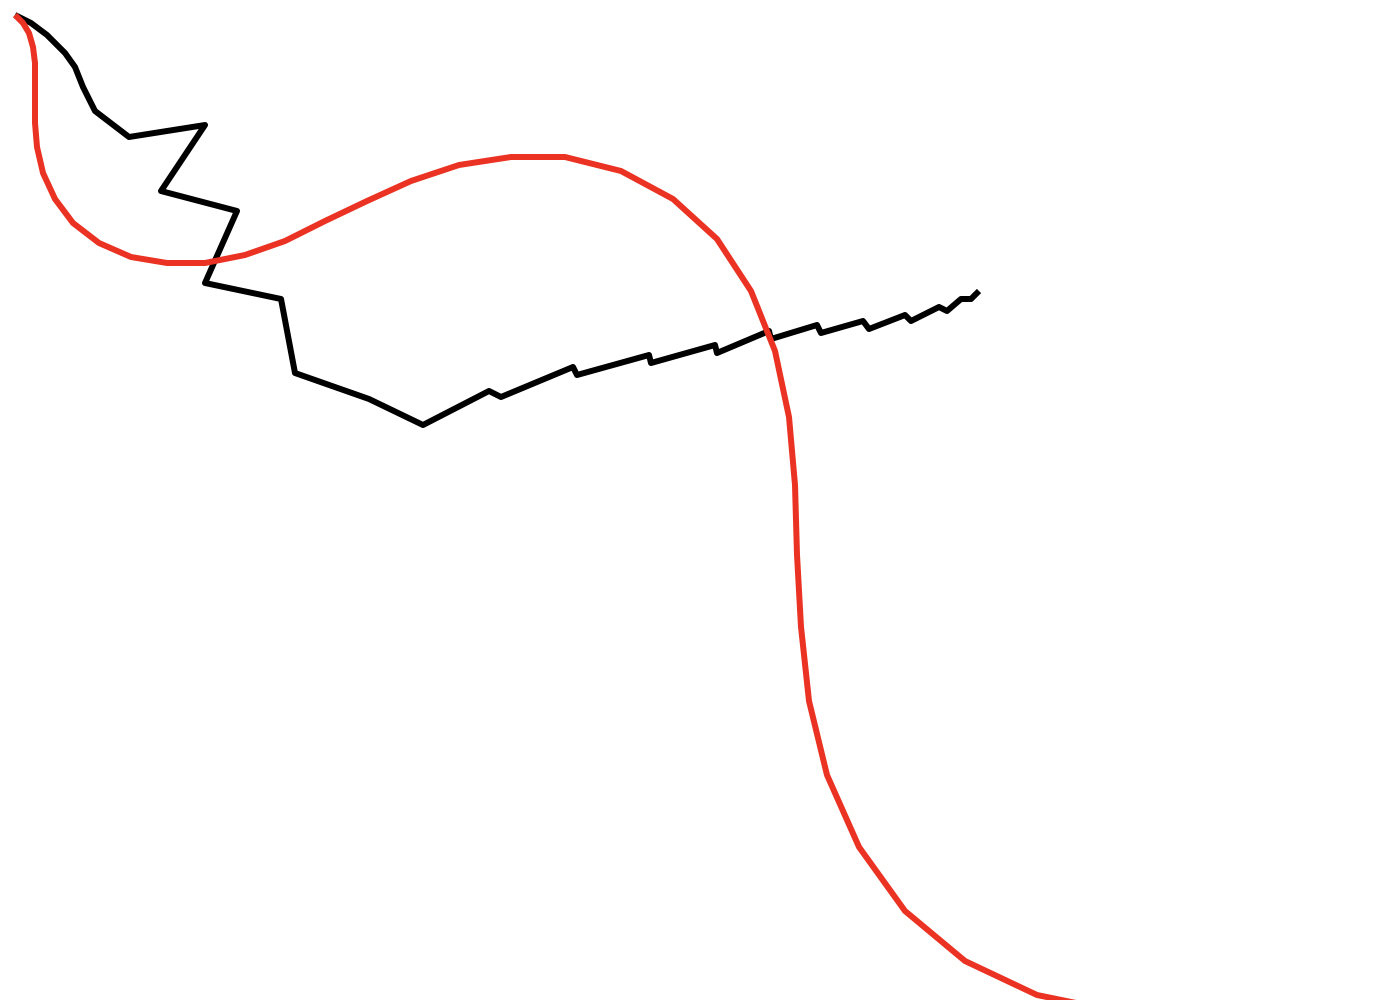
\includegraphics[width=\textwidth]{images/ddpg_results/envs_S3_S4_S5/S3_A2_R3_curve_A.png}
         \caption{$curve\_A$}
     \end{subfigure}
     \hfill
     \begin{subfigure}[b]{0.31\textwidth}
         \centering
         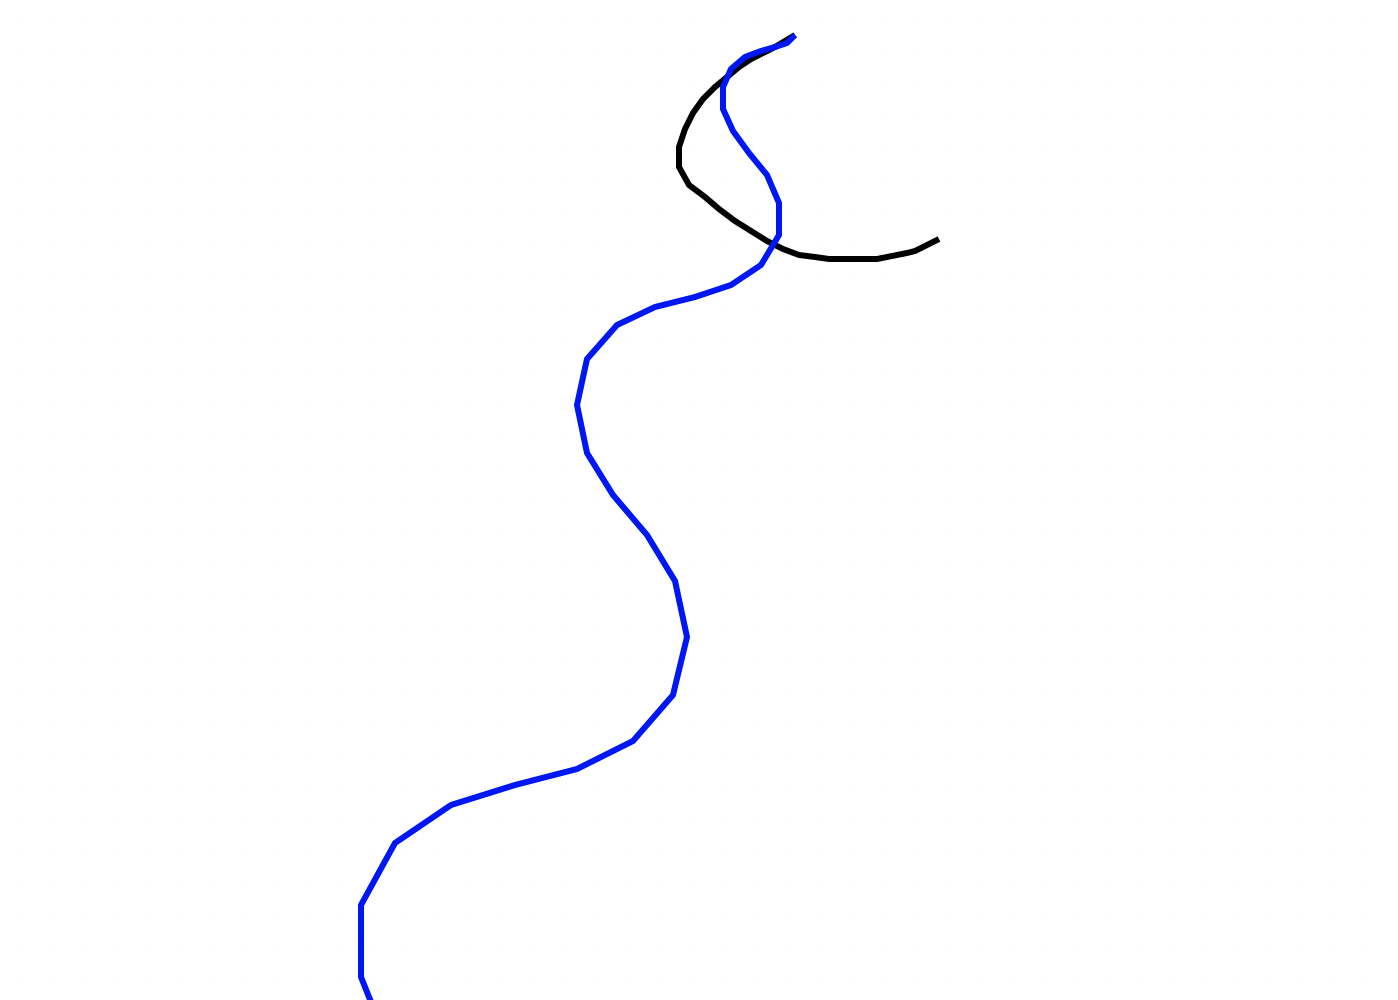
\includegraphics[width=\textwidth]{images/ddpg_results/envs_S3_S4_S5/S3_A2_R3_curve_B.png}
         \caption{$curve\_B$}
     \end{subfigure}
     \hfill
     \begin{subfigure}[b]{0.31\textwidth}
         \centering
         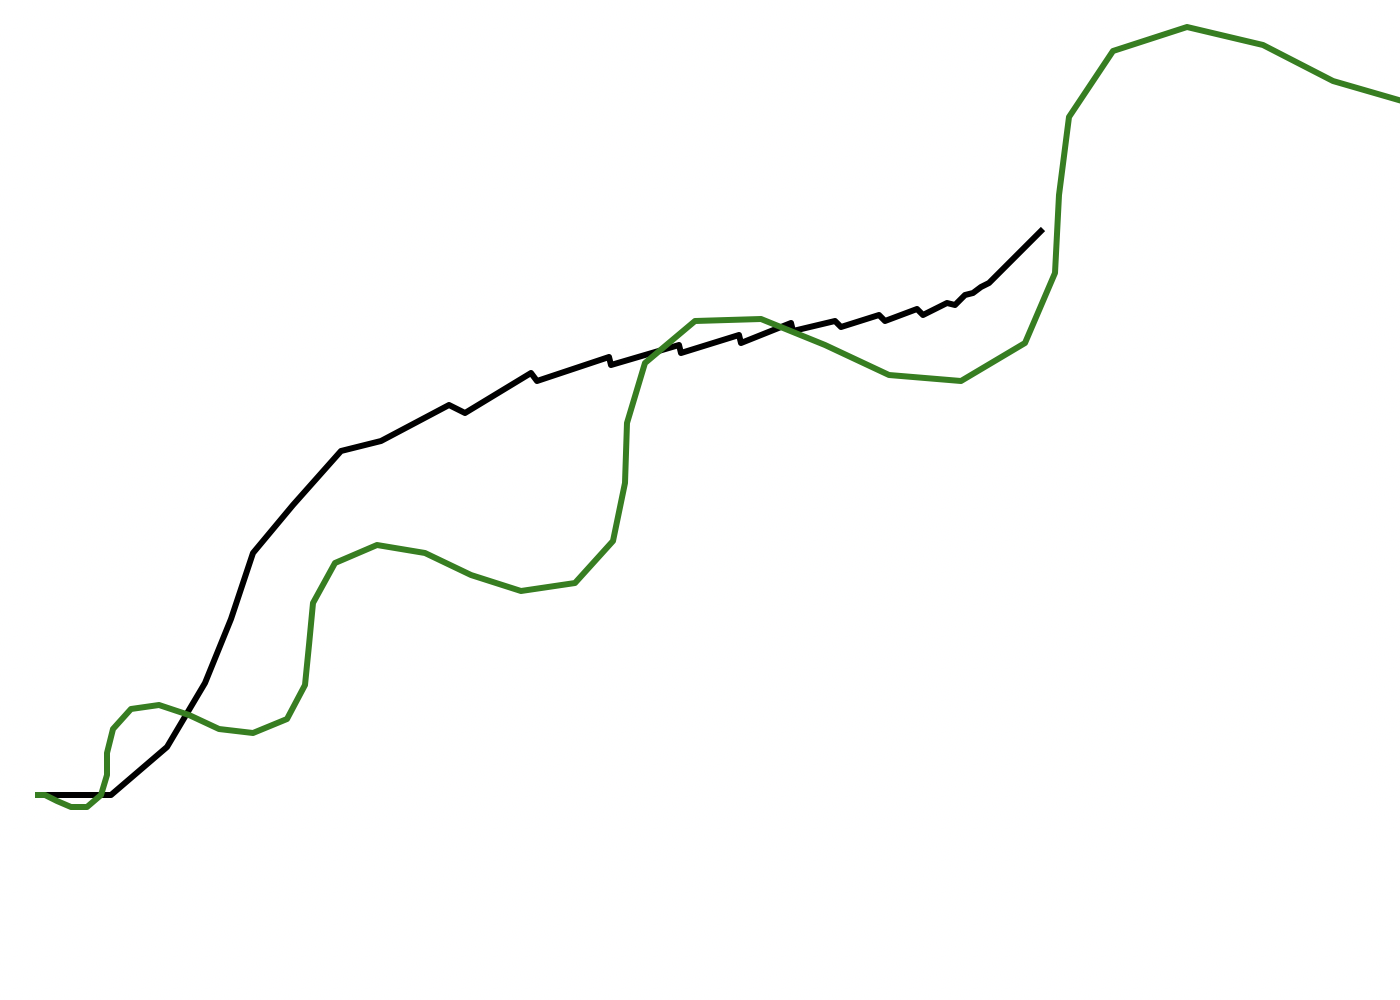
\includegraphics[width=\textwidth]{images/ddpg_results/envs_S3_S4_S5/S3_A2_R3_curve_C.png}
         \caption{$curve\_C$}
     \end{subfigure}
        \caption{$S3\_A2\_R3$ using $\sigma=0.15$ and a replay buffer size of $N=5\cdot 10^4$.}
        \label{fig:advCurves2}
\end{figure}


\begin{figure}[H]
     \centering
     \begin{subfigure}[b]{0.31\textwidth}
         \centering
         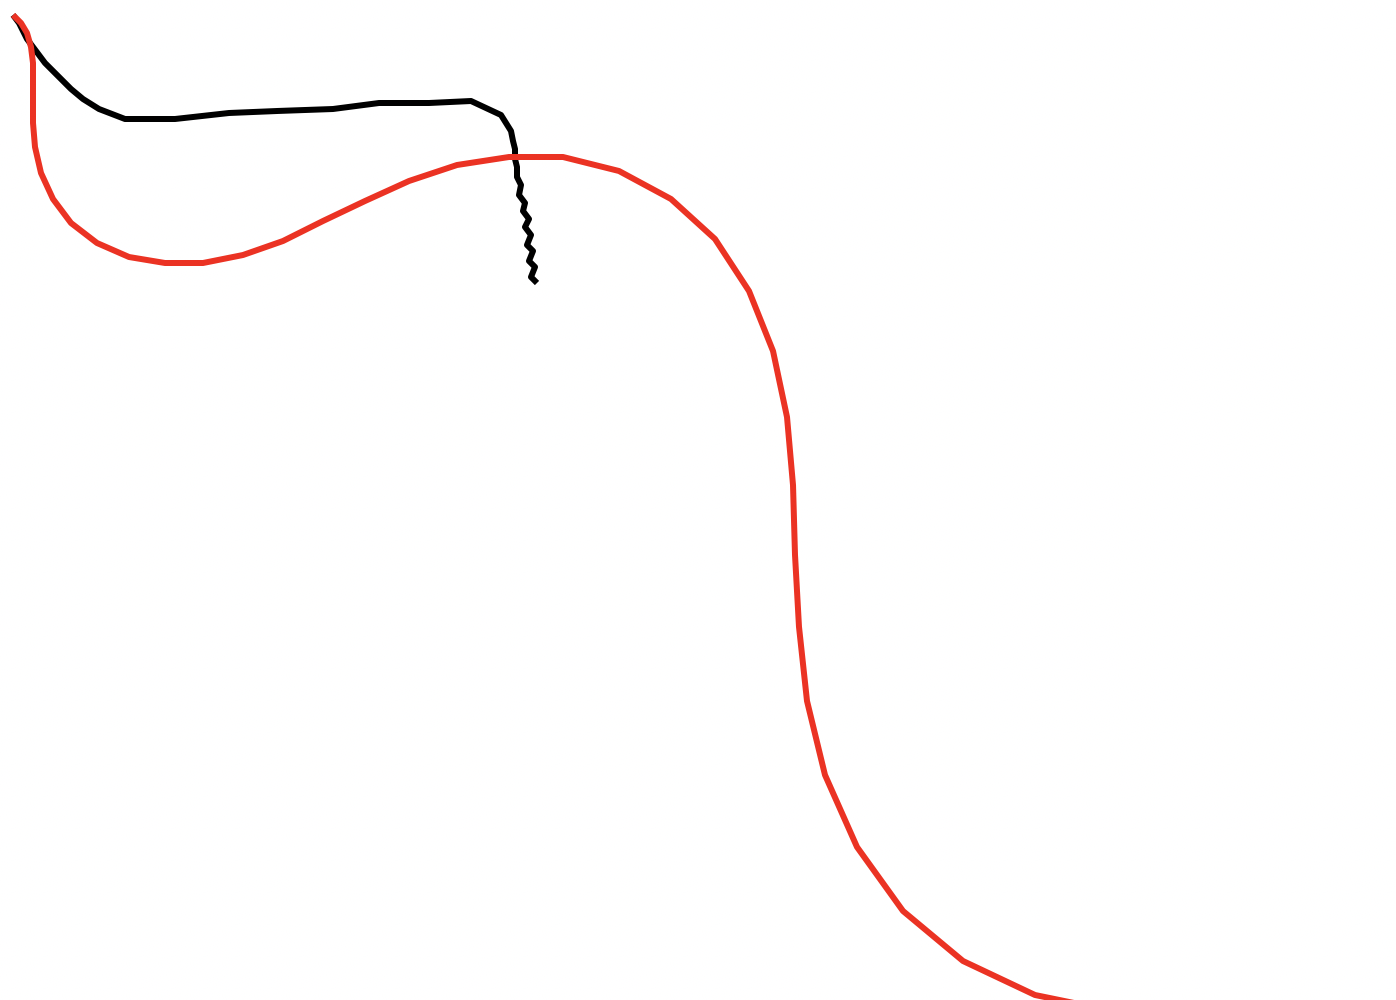
\includegraphics[width=\textwidth]{images/ddpg_results/envs_S3_S4_S5/S5_A2_R3_curve_A.png}
         \caption{$curve\_A$}
     \end{subfigure}
     \hfill
     \begin{subfigure}[b]{0.31\textwidth}
         \centering
         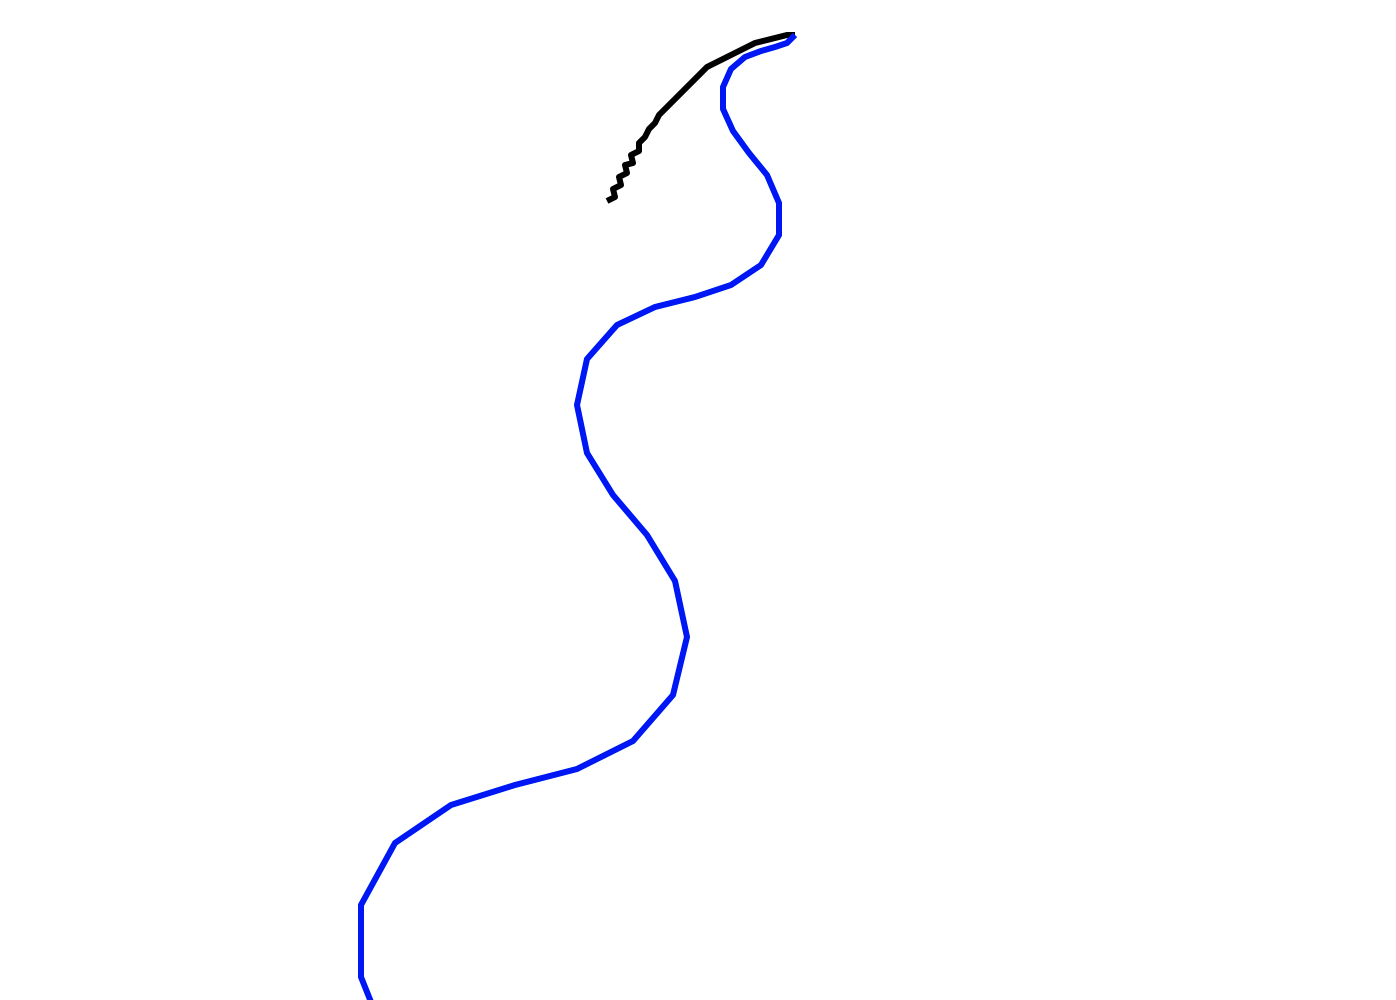
\includegraphics[width=\textwidth]{images/ddpg_results/envs_S3_S4_S5/S5_A2_R3_curve_B.png}
         \caption{$curve\_B$}
     \end{subfigure}
     \hfill
     \begin{subfigure}[b]{0.31\textwidth}
         \centering
         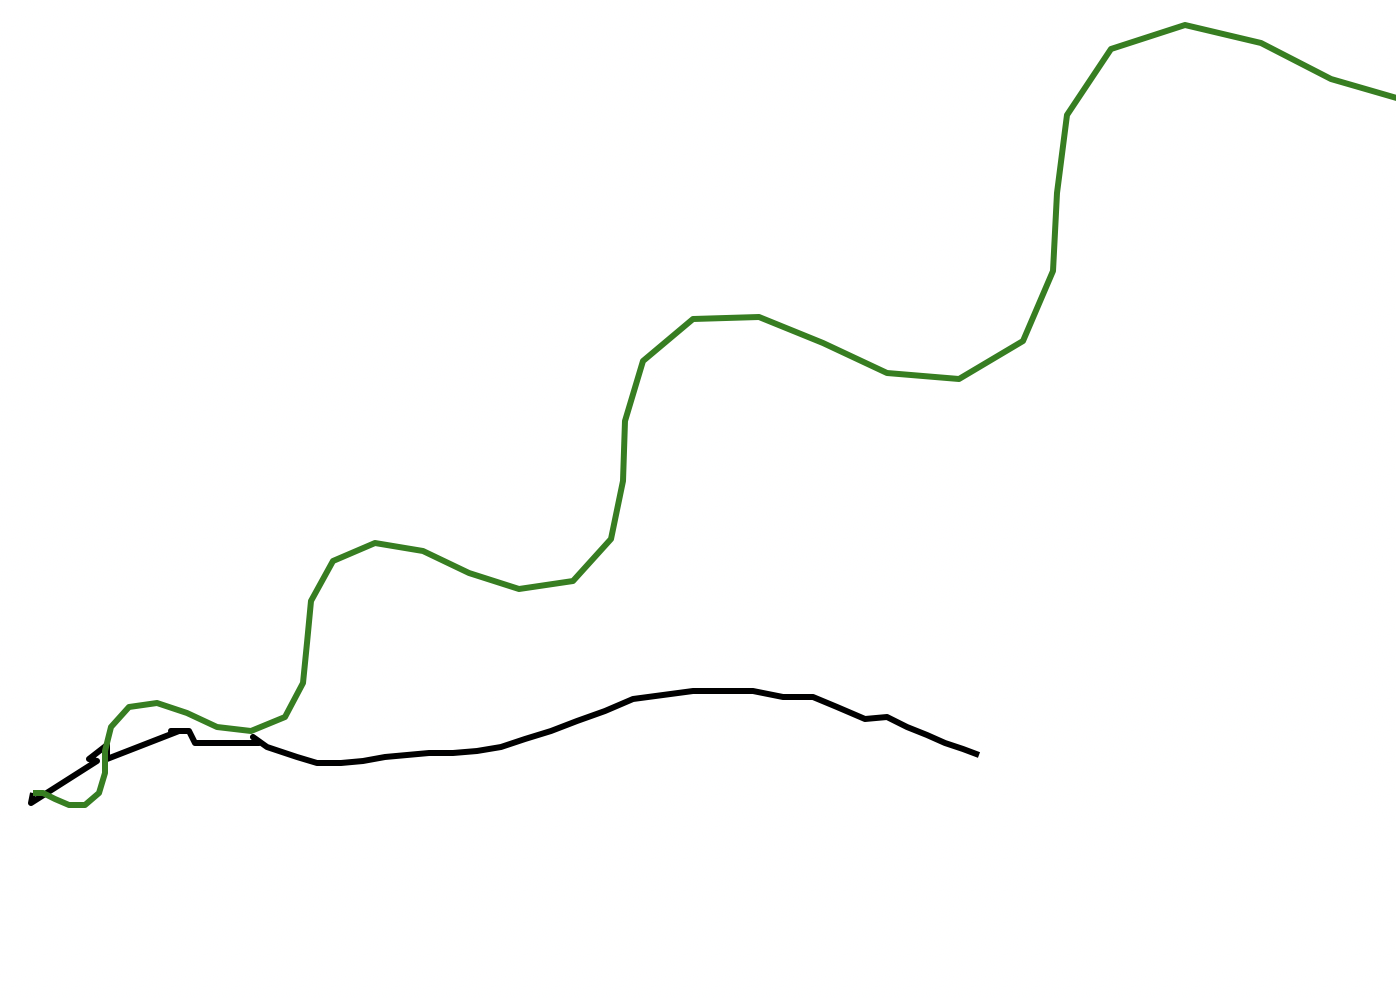
\includegraphics[width=\textwidth]{images/ddpg_results/envs_S3_S4_S5/S5_A2_R3_curve_C.png}
         \caption{$curve\_C$}
     \end{subfigure}
        \caption{$S5\_A2\_R3$ using $\sigma=0.15$ and a replay buffer size of $N=5\cdot 10^4$.}
        \label{fig:advCurves3}
\end{figure}
\newpage
The outcome illustrated in Fig. \ref{fig:advCurves1}, \ref{fig:advCurves2}, and \ref{fig:advCurves3} allow us to conclude that DDPG is not able to recover the direct optimal mapping in order to generate representative trajectories. No combination of replay buffer size, exploration magnitude, reward function, or applicable state representation shows respectable performance to the task. Still, there are some findings. One of them is the setting of $\sigma$, as a value above $0.3$ heavily impacts the performance negatively. Next, the replay buffer size shows no major effect on the outcomes, with $N=5 \cdot 10^4$ providing the best results. Besides that, the switch from identical learning rates for the actor and critic networks does indeed improve the performance of DDPG slightly (we include one experimental setup with the same learning rates in the appendix). A customization of the source code from the used library Stable-Baselines3 was necessary to allow for this usage of different learning rates. Moreover, the reward function $R3$ that sends out non-zero feedback at every time step provides better results than $R1$ and $R2$. Non-zero feedback is sent out every time step because the maximum distance for a positive reward is $100$, and during the training phase an episode is prematurely ended if the agent drifts apart from the GT more than $100$ pixels. Receiving feedback which directly translates to current distance to the GT, the agent has a supplementary indirect feature which helps to identify the current snapshot of the environment.
\par
With that in mind, we construct $S4$, which adds the current distance to the GT as a primary feature to the state space. During the initial experiment setup and the corresponding results shown in Tab. \ref{tab:resultsK3}, $S4$ yields the best performance, with $S4\_A2\_R3$ having an average distance of 80. In relation to the other state representations $S3$ and $S5$, this is a great improvement and thus gives a hint about why the other representations fail the task. But first, we visualize the proposed tracks by the fully trained agent in the upcoming Fig. \ref{fig:advCurves5}

\begin{figure}[H]
     \centering
         \includesvg[width=0.9\textwidth]{images/ddpg_results/envs_S3_S4_S5/ddpg_S4_A2_R3_K9.svg}
        \caption{Distances between the path proposed by the agent and the GT over time. $\sigma = 0.15$ and $N=5\cdot 10^4$.}
        \label{fig:advCurves4}
\end{figure}


\begin{figure}[H]
     \centering
     \begin{subfigure}[b]{0.31\textwidth}
         \centering
         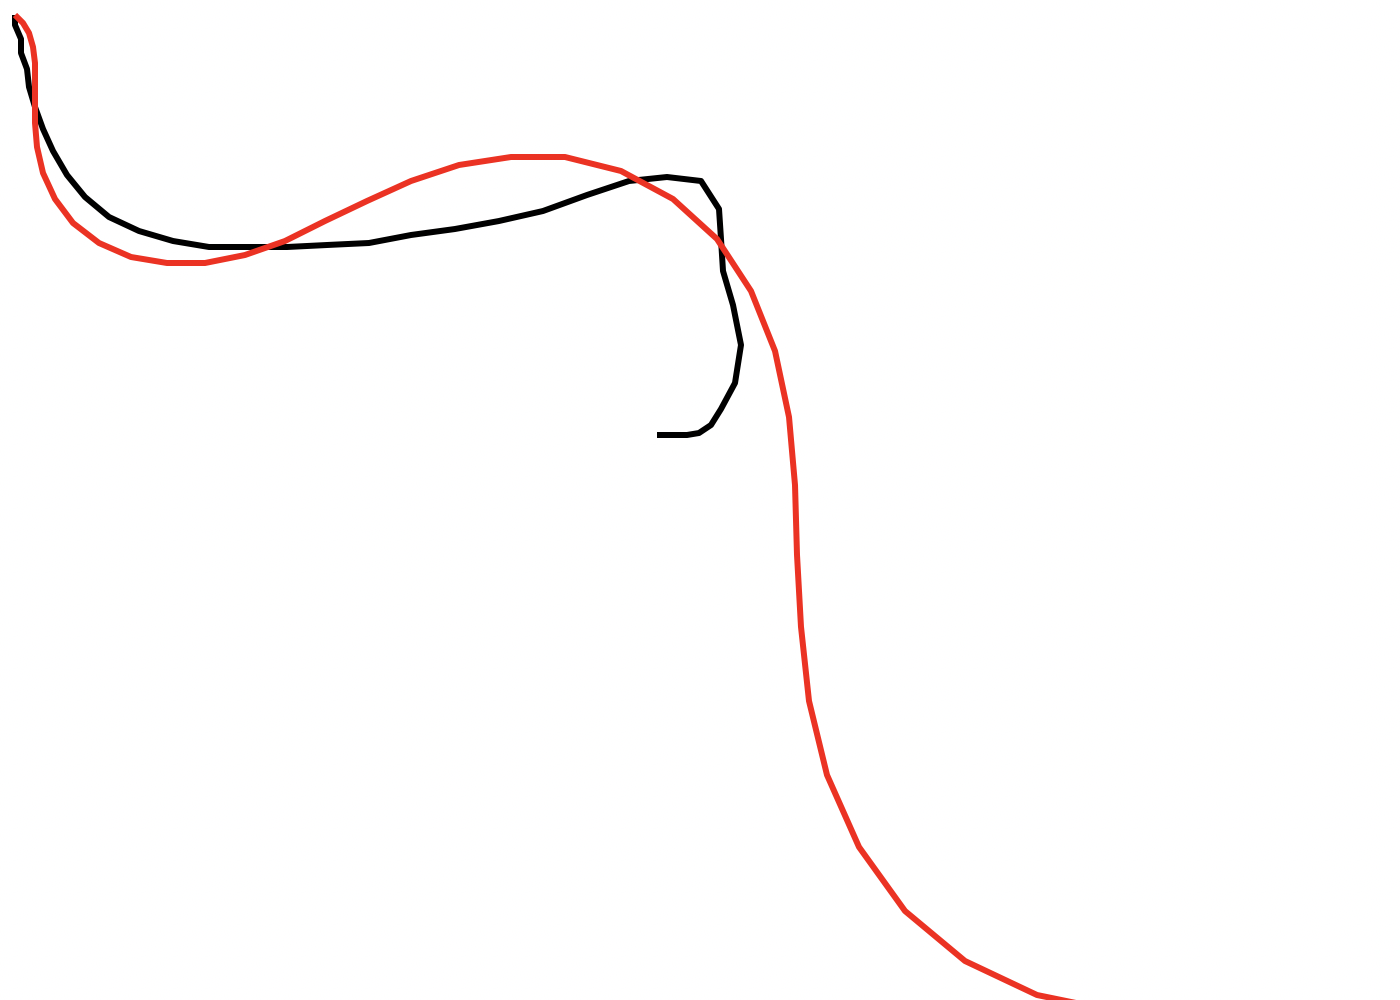
\includegraphics[width=\textwidth]{images/ddpg_results/envs_S3_S4_S5/S4_A2_R3_curve_A.png}
         \caption{$curve\_A$}
     \end{subfigure}
     \hfill
     \begin{subfigure}[b]{0.31\textwidth}
         \centering
         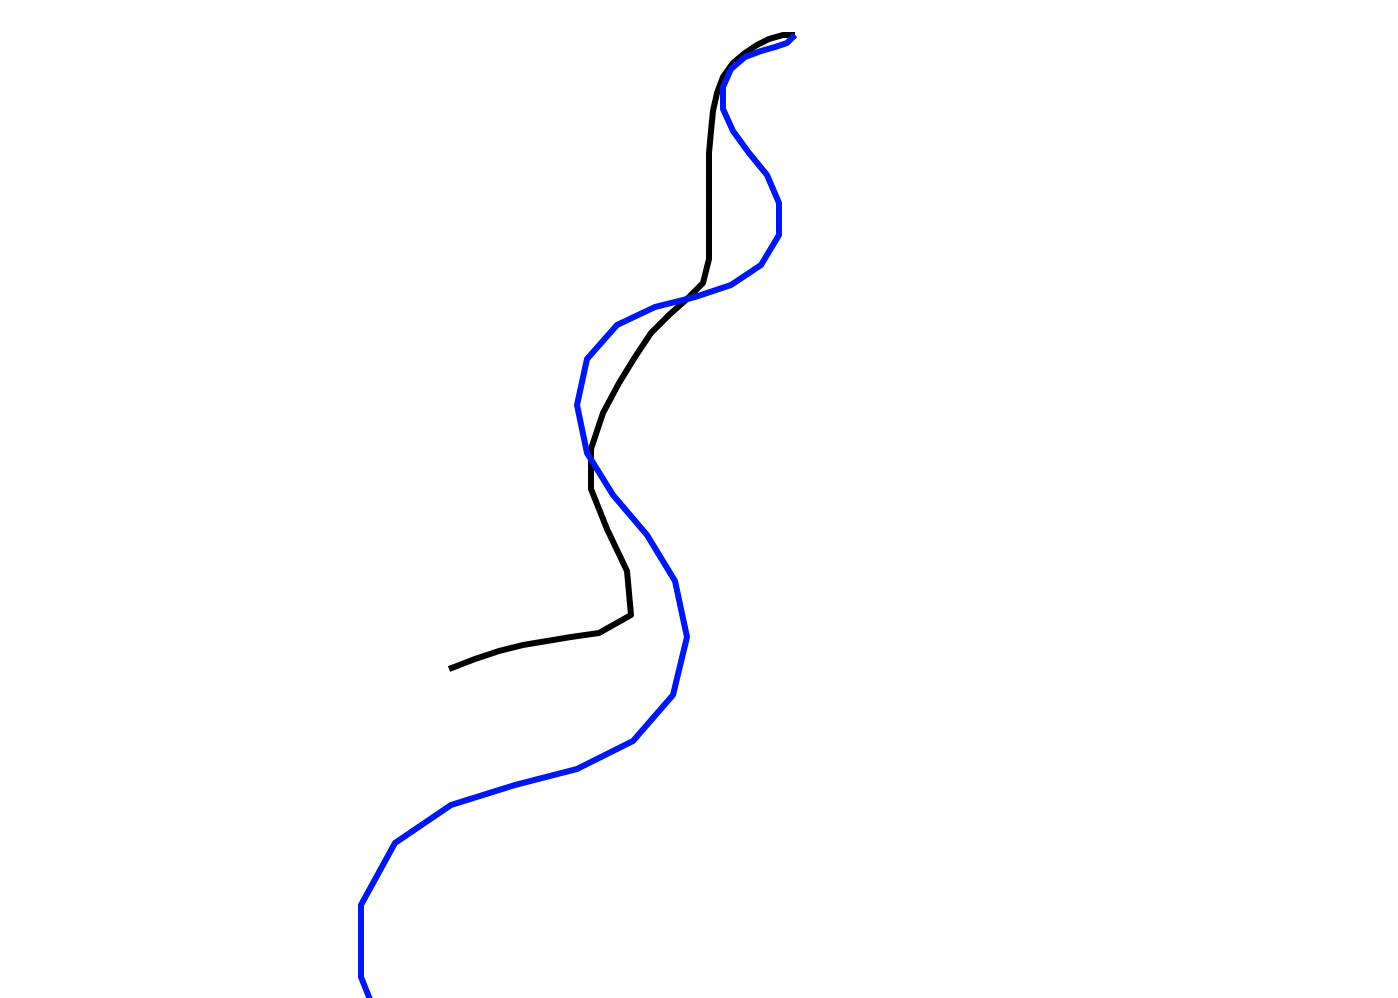
\includegraphics[width=\textwidth]{images/ddpg_results/envs_S3_S4_S5/S4_A2_R3_curve_B.png}
         \caption{$curve\_B$}
     \end{subfigure}
     \hfill
     \begin{subfigure}[b]{0.31\textwidth}
         \centering
         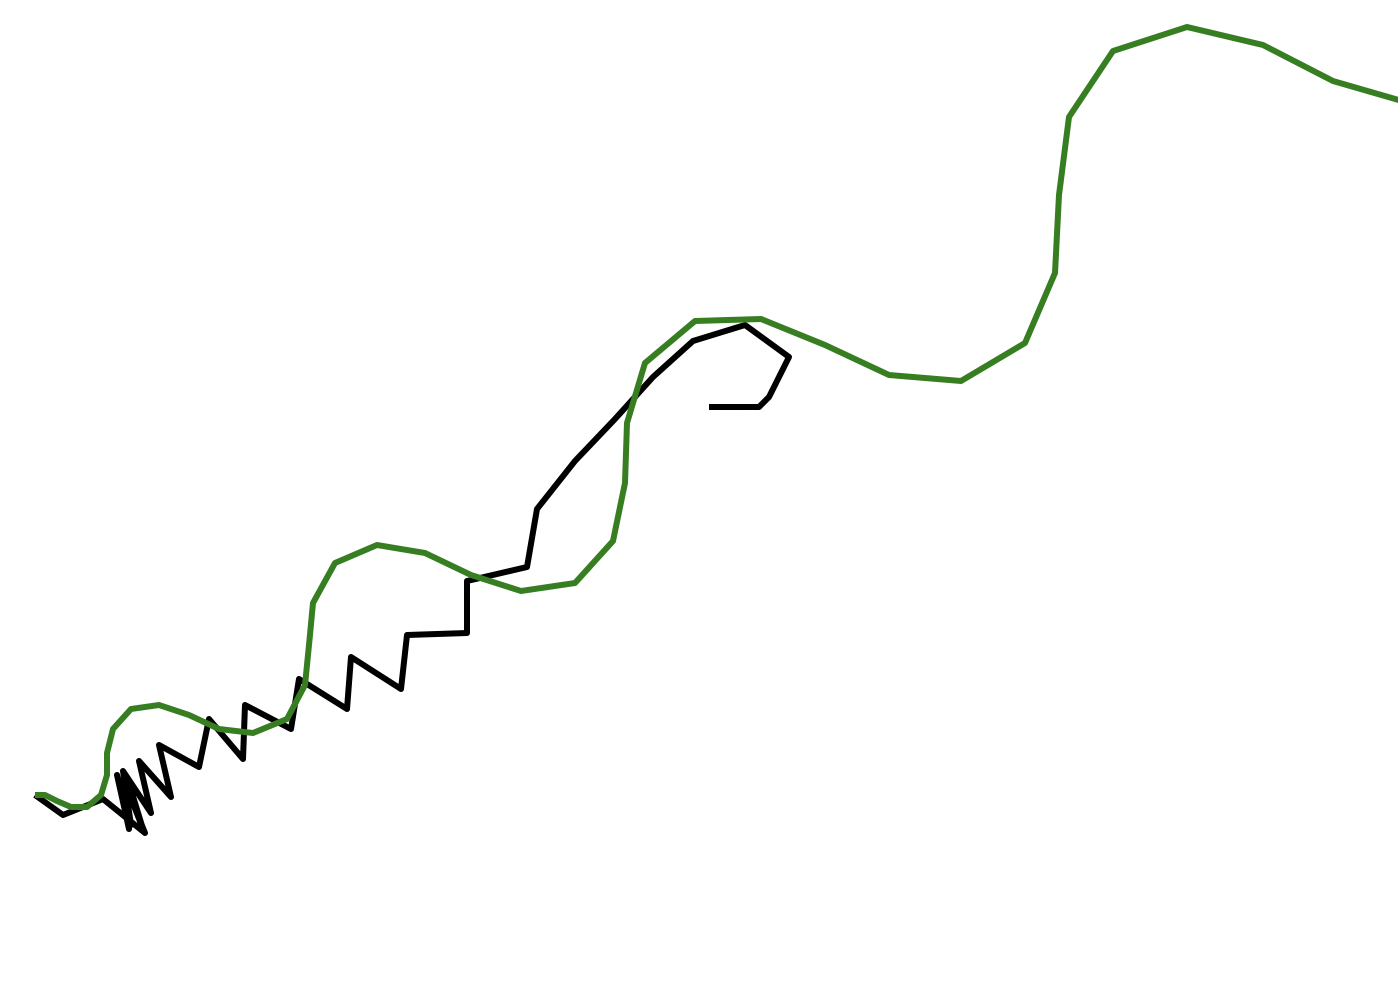
\includegraphics[width=\textwidth]{images/ddpg_results/envs_S3_S4_S5/S4_A2_R3_curve_C.png}
         \caption{$curve\_C$}
         \label{fig:a5c}
     \end{subfigure}
        \caption{$S4\_A2\_R3$ using $\sigma=0.05$ and a replay buffer size of $N=5\cdot 10^4$.}
        \label{fig:advCurves5}
\end{figure}

Although it has the best performance, $S4$ is still not able to fulfill the task on an acceptable level, which can be seen in Fig. \ref{fig:advCurves5}. However, in contrast to the previous visualized behaviors, the agent does not fluctuate in one area and is also able to generate paths that stay in the same region as the GT curve while heading in the same overall direction (best seen in Fig \ref{fig:a5c}).
\par
The reason behind the improved performance is the extended state space by a component that enhances the ability of the agent to separate between different snapshots of the environment during each episode. Previous state representations fail catastrophically because the replay buffer is filled with inconsistent feedback about state-action pairs that do seem to be the same in the eyes of the agent. For example, if the agent chooses a good action right at the beginning of an episode with fitting values of heading and speed while receiving $\{x, y, heading, speed\}$ as in $S3$, this transition gets saved into the replay buffer. This specific transition has a high positive reward because the next position of the agent is close to the GT. Assuming that the agent explores enough for the next time steps and ends up in the same state as the very first one. Even if the agent now chooses the perfect action again, the GT has already moved away, and in return the agent would be rewarded with a smaller value for this particular state-action pair than already saved in the replay buffer. As the episode continuous, the replay buffer gets overwhelmingly filled with transition tuples that indeed include the first state but with different reward values, which get smaller over time. Being filled with predominantly bad reward values for this specific state-action pair, the replay buffer is also responsible for the low Q-value assignment by the critic network because it is trained by randomly sampling the buffer.
\par
Adding the distance to the GT changes this behavior, as the agent is able to distinguish between different states during an episode and is also able to distinguish between different curves. Overall, we conclude that DDPG needs a very rich feature space that truly represents the environment at a certain time step and also allows the agent to choose actions to recover from bad states. In this instance, a high distance could potentially lead to a higher suggested value of speed. In the state representation of $S3$, there is no such thing as a recovery mechanism because the agent is unaware of the GT through the state space and only receives information about the GT position in the form of the reward signal. For direct policy learning, with the requirement of acting perfectly, as in conducting the perfect actions to follow the GT position at all time steps, DDPG seems to be the wrong approach. Especially, when the environment changes in the testing phase, because the GT is not present anymore and thus reducing the number of possible features.
\par
Besides the challenges of necessary feature engineering and state representation, we experience DDPG to be very susceptible to a variety of hyperparameters. From replay buffer sizes, exploration noise and learning rates, to the optimal reward function and different seeds, the performances of the separate runs varied significantly.
    \newpage
    \subsection{Applying Imitation Learning} \label{subchap:applyBC}
    As already described in the subchapters \ref{subchap:nature} and \ref{subchap:reinterpreting}, it is also possible to express the overall task as an imitation problem, where the agent directly tries to mimic the underlying policy of a human expert—the captain. In the case of behavioral cloning, the agent does not explore the state space nor receives rewards anymore, but instead learns the state and action distributions in a supervised manner. Here, the dataset consists of simplified transition tuples of just $(s_t, a_t)$ where the features of $s_t$ are the input to the policy network and $a_t$ marks the desired output. The dataset is generated by recording the current state of the GT, as well as the next heading and speed values as expert action, based on the presented functions that produce $curve\_A$, $curve\_B$ and $curve\_C$, i.e., Eq. \ref{eq:curve_A}.
\par
When exposing behavioral cloning to the same task of generating trajectories that are identically to the GT curves, it shows better performance in contrast to DDPG throughout all experiment setups. This is indeed an expected outcome, as a big enough neuronal network should be able to overfit to the training data and thus learn the perfect mapping of states to actions. Nevertheless, different network architectures show deviating performances, which suggests the need for further investigations. In this context, we conduct a series of experiments, testing different learning rates and network settings. The results for all these experiments can be found in the appendix in section \ref{appendix:curveResults}.
\par
We found out that the default network architecture of the used library \textit{imitation} of $n_{h}^{1}=100$ and $n_{h}^{2}=100$ can be improved, not only by the raw amount of neurons in each hidden layer, but also by the proportion of the different hidden layers. Generally, we notice that having consecutive hidden layers with reducing amounts of neurons yield better results than an equal proportion regardless of the number of neurons. For the real-world applicable state representation $S3$, the best outcome is achieved by a fully-connected neuronal network comprised of $n_{h}^{1}=256, n_{h}^{2}=128$ and $n_{h}^{3}=64$, which is trained for 15k epochs with a learning rate of $\alpha = 10^{-5}$. The upcoming Figs. \ref{fig:bcCurves1} and \ref{fig:bcCurves2} visualize the behavior of the trained policy network that has a performance of $2.92 \pm 2.28$. Please note, that the y limits of the graph in Fig. \ref{fig:bcCurves1} are different from the graphs of the previous chapter.

\begin{figure}[H]
     \centering
         \includesvg[width=0.9\textwidth]{images/bc_curve_results/bc_S3_A2_256_128_64_5lr.svg}
        \caption{Performance of behavioral cloning over time during the three different episodes. Learning rate $\alpha = 10^{-5}$ trained for 15k epochs with a network architecture of $n_{h}^{1}=256, n_{h}^{2}=128$ and $n_{h}^{3}=64$.}
        \label{fig:bcCurves1}
\end{figure}


\begin{figure}[H]
     \centering
     \begin{subfigure}[b]{0.31\textwidth}
         \centering
         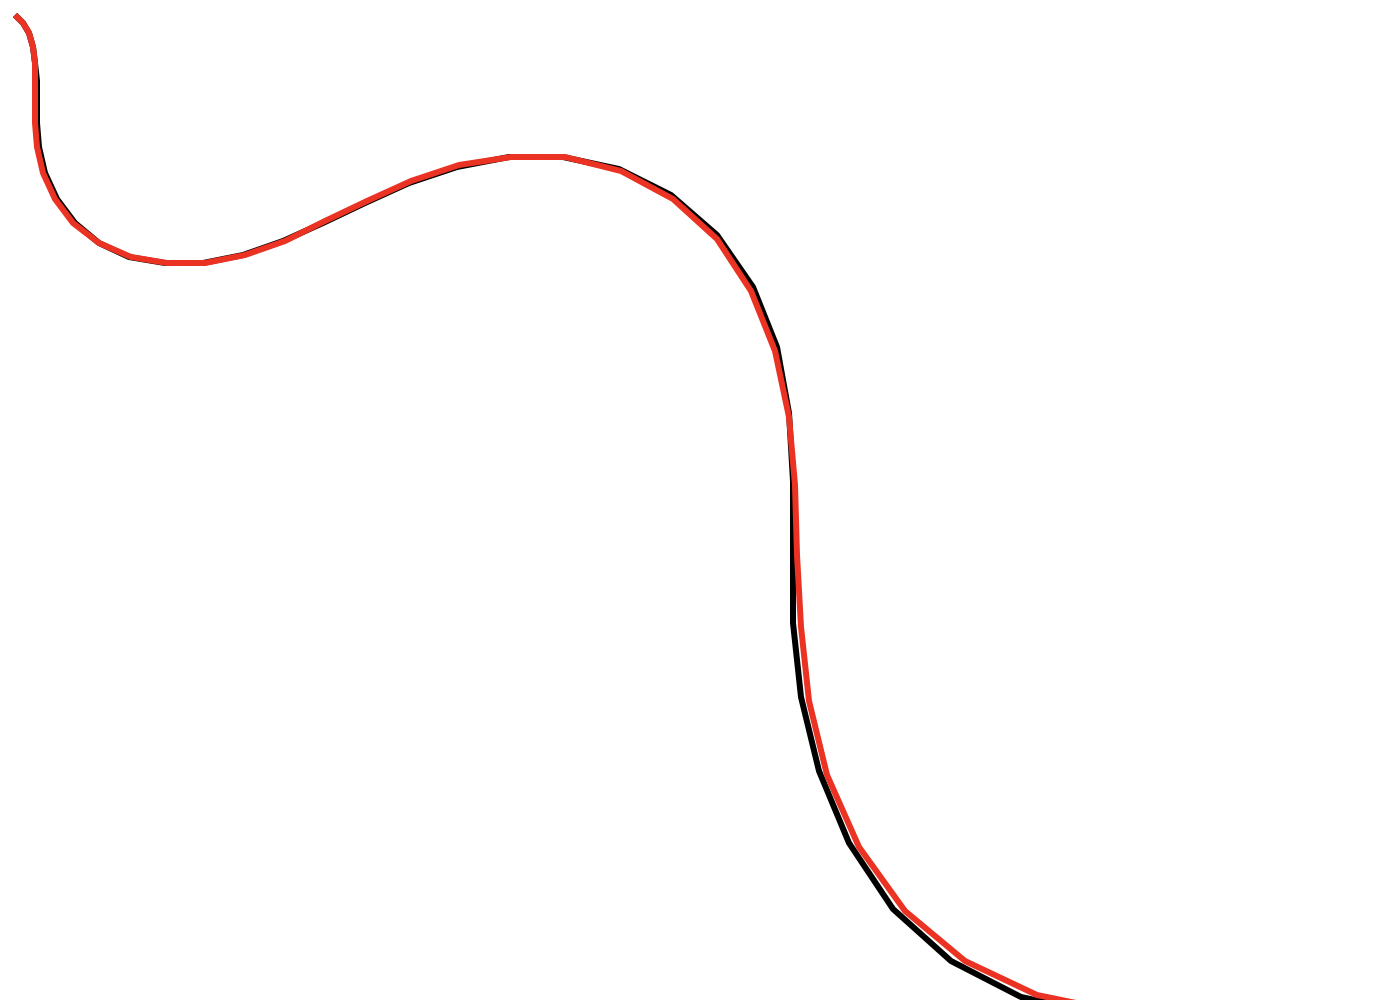
\includegraphics[width=\textwidth]{images/bc_curve_results/S3_A2_256_128_64_curve_A.png}
         \caption{$curve\_A$}
     \end{subfigure}
     \hfill
     \begin{subfigure}[b]{0.31\textwidth}
         \centering
         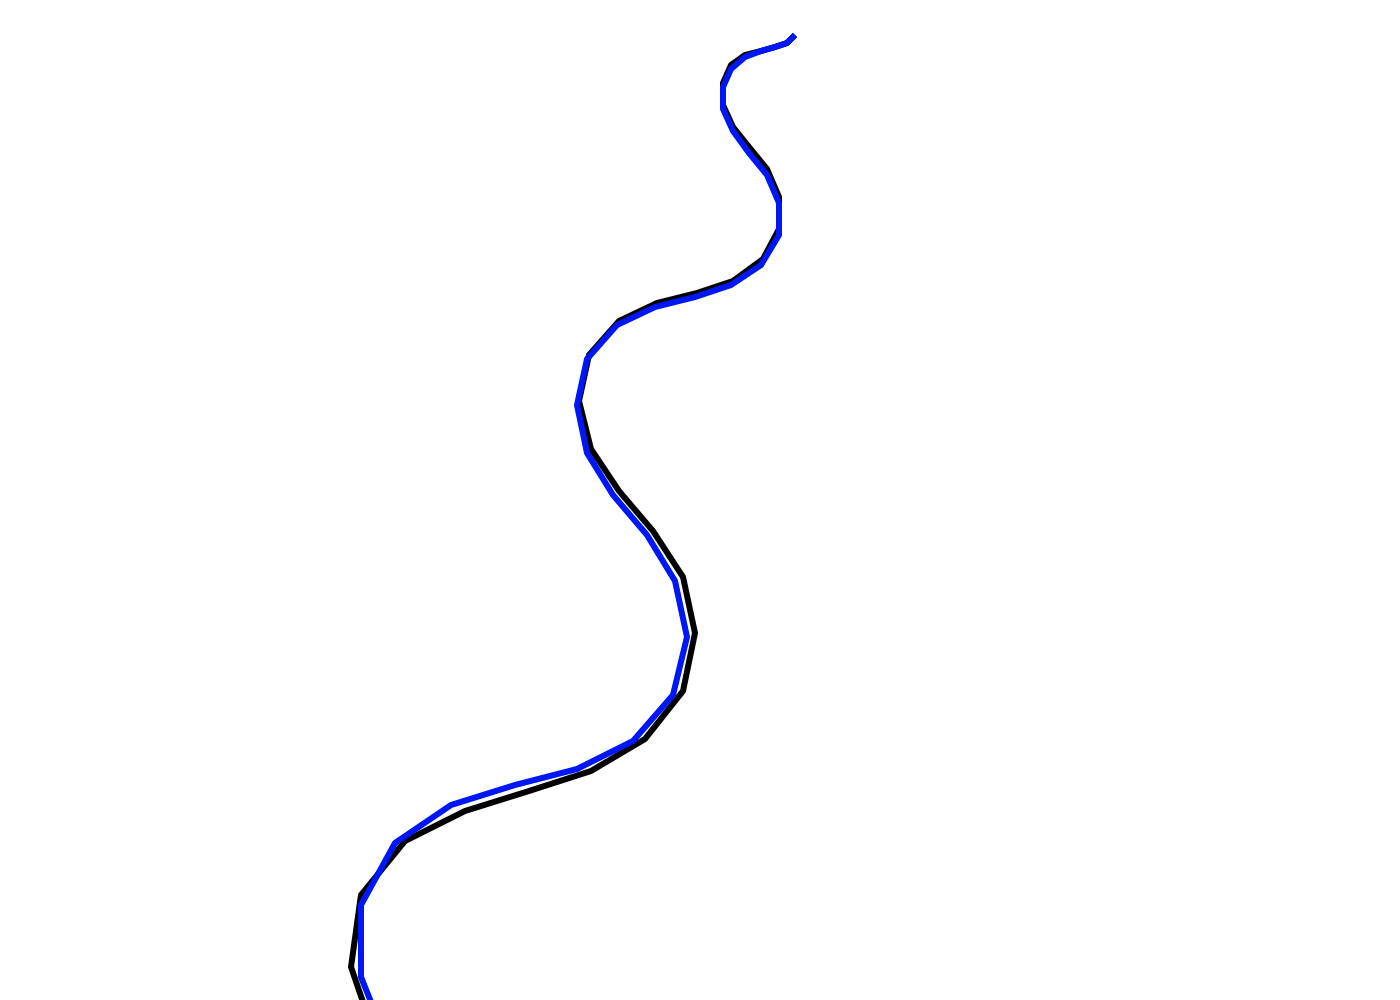
\includegraphics[width=\textwidth]{images/bc_curve_results/S3_A2_256_128_64_curve_B.png}
         \caption{$curve\_B$}
     \end{subfigure}
     \hfill
     \begin{subfigure}[b]{0.31\textwidth}
         \centering
         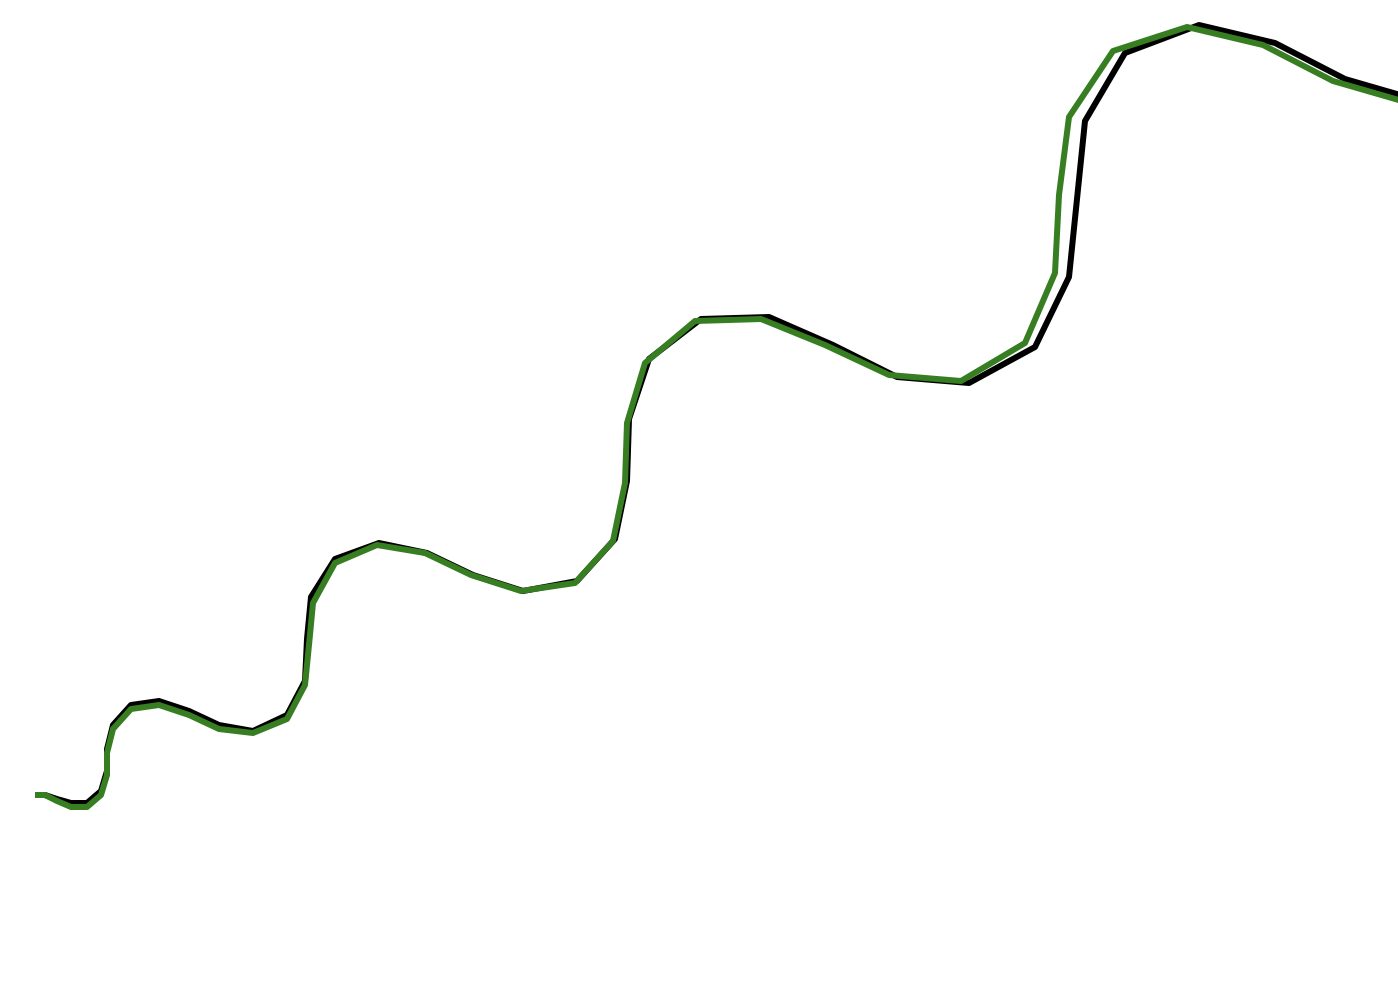
\includegraphics[width=\textwidth]{images/bc_curve_results/S3_A2_256_128_64_curve_C.png}
         \caption{$curve\_C$}
     \end{subfigure}
        \caption{$S3\_A2$, learning rate $\alpha = 10^{-5}$ trained for 15k epochs with a network architecture of $n_{h}^{1}=256, n_{h}^{2}=128$ and $n_{h}^{3}=64$.}
        \label{fig:bcCurves2}
\end{figure}


    \subsection{Libraries}
    Although we implemented the DDPG algorithm from scratch and tested its correctness by applying it to the classic control problem "MountainCarContinuous-v0" \cite[]{moore1990efficient}, we will still make use of sophisticated external libraries for deep-, reinforcement- and imitation learning. Those libraries are exclusively open-source, actively maintained by thousands of contributors and well known in the research community (based on respective numbers from Github in contributors and stars). To give an overview of the most important libraries used in this thesis, we list and describe their functionality in the upcoming subchapters.

\subsubsection{PyTorch}
PyTorch \cite[]{NEURIPS2019_9015} offers the foundation of handling tensor computation and the building of deep neuronal networks. Being implemented in C++ with strong GPU acceleration, its Python API is not as high-level as e.g. the one of \textit{Keras}. On the one hand this might discourage certain end user because more boilerplate code has to be written. However, on the other hand its  “everything is a just a program” philosophy \cite[p.~4]{NEURIPS2019_9015} of treating layers, optimizers, activations or data loaders as functions which can be composed in any arbitrary way, allows for great flexibility when it comes to assemble complex neuronal network architectures (e.g. loops or recursive functions). In order to compute the gradients of arbitrary models and user defined functions, PyTorch uses a method called "automatic differentiation" \cite[p.~5]{NEURIPS2019_9015}. In short, this method saves all operations and interim tensors of the forward pass in a direct directed acyclic graph (DAG) to calculate the respective gradients and apply the chain rule during backprogragation. PyTorch records the series of user functions and assembles the DAG at runtime by operation overloading.

\subsubsection{Stable-Baselines3}


\subsubsection{imitation}
The \textit{imitation} library \cite[]{wang2020imitation} implements popular Imitation Learning algorithms on top of Stable-Baselines3 and even gets referenced by the official SB3 documentary. In its current state, this library includes Behavioral Cloning, DAgger, Maximum Causal Entropy Inverse Reinforcement Learning, Adversarial Inverse Reinforcement Learning, Generative Adversarial Imitation Learning and Deep RL from Human Preferences.

\subsubsection{MovingPandas}\label{subchap:movingPandas}
\textit{MovingPandas} \cite[]{graser2019movingpandas} is built on top of \textit{GeoPandas} \cite[]{kelsey_jordahl_2020_3946761} and offers classes and functions for movement data analysis. To be more precise, we use MovingPandas to transform raw AIS records into trajectories and make use of its powerful high-level functionalities such as "Splitters" and "Cleaners" to preprocess and generate our final dataset of real-world vessel paths.
    
\newpage
\section{Predicting Real-World Vessel Paths}\label{chap:realworld}
This chapter presents the setup, performance and weakness of a system that should learn representative vessel trajectories in order to generate and predict future paths. The overall system is built based on the findings of the synthetic experiments which were deeply discussed in the previous chapter \ref{chap:synthetic}.
\par
First, the process of handling historical AIS data and extracting ship trajectories is displayed. The resulting dataset acts as ground truth (GT) in the custom environment which is explained in the next subchapter. Afterwards, a generic metric is introduced which in return is used to describe the performance of the system and to discuss the results. Finally, we trace and analyse supposedly bad predictions to potentially discover patterns which lead to bad performances.
    \subsection{Extracting Vessel Trajectories}
    In order to build a dataset containing real-world trajectories, we initially are in need of historical AIS data. Although, the AIS signal from every ship gets freely broadcasted and can be potentially received by anyone with a suitable receiver or antenna, we still struggled to obtain a raw dataset. Services like \textit{MarineTraffic} display live ship positions based on AIS data, but getting access to historical data involves a fee and a request, which in fact got ignored in our case. Even our friendly request for free historical AIS data for academic use at a local institution, the \textit{Maritime Safety and Security Centre} in Cuxhaven, got denied with a reference to a German law that requires every claimant to pay a fee.
\par
Fortunately, the DLR-MI has access to historical AIS data through a service called \textit{AISHub}, which allows its members to exchange AIS data. Thus, our raw dataset consists of four months of raw AIS signals from the year 2020 (first month of each quarter). To be more precise, for the recorded months January, April, July, and  October, over 5,93 million AIS messages are available that got sent by 2011 distinct ships (based on the amount of unique MMSIs). The observation window is spanned by longitude from $8\degree37.2'N$ to $8\degree59.1'N$ and latitude from $53\degree49.0'W$ to $53\degree71.9'W$.
\par
The process of filtering and extracting single vessel trajectories is done  in  conjunction  with  the  library \textit{MovingPandas} (see chapter \ref{subchap:movingPandas}) and can be summarized by the following steps:
\paragraph{1. Remove unwanted speed records.}
Prior to any conversion to intern class \textit{Trajectory} of MovingPandas, the raw AIS records get filtered by the speed over ground (SOG). The focus of this thesis is on moving ships that enter or leave the port, hence we remove records that indicate that a ship moves too slow ($<3$ knots). Additionally, we remove instances where a ship is speeding or the SOG value is unrealistic for the ship types we are most interested in ("passenger", "cargo", and "tanker"; $>30$ knots).


\paragraph{2. Extract provisionally trajectories.}
In the next step, we transform the raw AIS signals to trajectories respectively into a \textit{TrajectoryCollection}, an intern class from MovingPandas which holds multiple trajectories that in return are constructed based on the unique MMSI. 

\paragraph{3. Add artificial direction and speed.}
MovingPandas offers the functionality to add artificial values for the direction and speed purely based on the given geographic positions (longitude and latitude). We will add this information in addition to the SOG and COG values of the AIS signal because we do not use a dedicated ship simulation to calculate next ship positions. It is a matter of testing, if there is any noticeable difference in using the artificial values or the values given by the AIS signal. Our assumption is that if we take the positions as ground truth for the calculation of direction and speed by using the functions of MovingPandas, we utilize the exact some transition dynamics when it comes to calculating next ship positions in the custom AIS environment.

\paragraph{4. Remove outliers.}
MovingPandas allows the cleaning of outliers based on the interquartile range. This rather simple approach works by first calculating the range between the first and third quartile. Afterwards, this range is multiplied by a constant $\alpha$, which in our case is $3$ solely because MovingPandas suggests this value in the corresponding function description. The resulting value is subtracted from the first quartile and added to the third quartile. All values outside the range of those two values are marked as outliers and get removed.

\paragraph{5. Split trajectories by time gaps.}
Trajectories are constructed by MovingPandas entirely based on the MMSI. Under the hood, MovingPandas simply groups the input data frame by the MMSI, which eventually leads to a single trajectory per unique ship. To be able to separate those single trajectories into voyages, MovingPandas offers a variety of \textit{Splitters}. The first \textit{Splitter} we will apply is the \textit{ObservationGapSplitter}, which splits trajectories that have too long gaps in consecutive AIS signals. Not only will this operation extract unique voyages of ships, it will also remove disrupted signals which would require long phases of interpolated values.
We chose a minimum time delta per gap of five minutes.

\paragraph{6. Split trajectories by stops.}
Visualizations of the trajectories after the previous step still show ships that do not move towards a destination and are probably anchoring or wait in a floodgate. One example of those unwanted tracks are the tugs that lie in the tug harbor. Their AIS signal is disturbed, resulting in positions that jump arbitrary and thus being recognized as moving. To fix this issue and remove those fake voyages, we apply the \textit{StopSplitter}. This class takes in all tracks and splits them by ships that stay within a predefined area for a minimum duration. In our case, we remove and split ships that stay within an area of 15 meters in diameter for at least three minutes.


\paragraph{7. Remove short trajectories.}
We solely keep trajectories that have a length of more than 1500 meters to  exclude ships that move "inside" the port until reaching the floodgates and to create a dataset consisting predominantly of trajectories documenting the way large ships leave or approach the port from the North Sea.

\paragraph{8. Up sample and unify time intervals.}
Finally, all records of every trajectory get resampled to have fixed time intervals of ten seconds. Missing values are linearly interpolated. The idea behind this up sampling is that the time component gets incorporated directly into the dataset and does not have to be provided in the state representation. Without explicitly knowing, the agent will always take actions that lead to the next state ten seconds into the future.
\par

After the extracting process, the resulting dataset, which we refer to as "all ships"-dataset, consists of 25,019 trajectories, with a subset of 300 voyages being shown in Fig. \ref{fig:tracks}.

\begin{figure}[H]
    \centering
    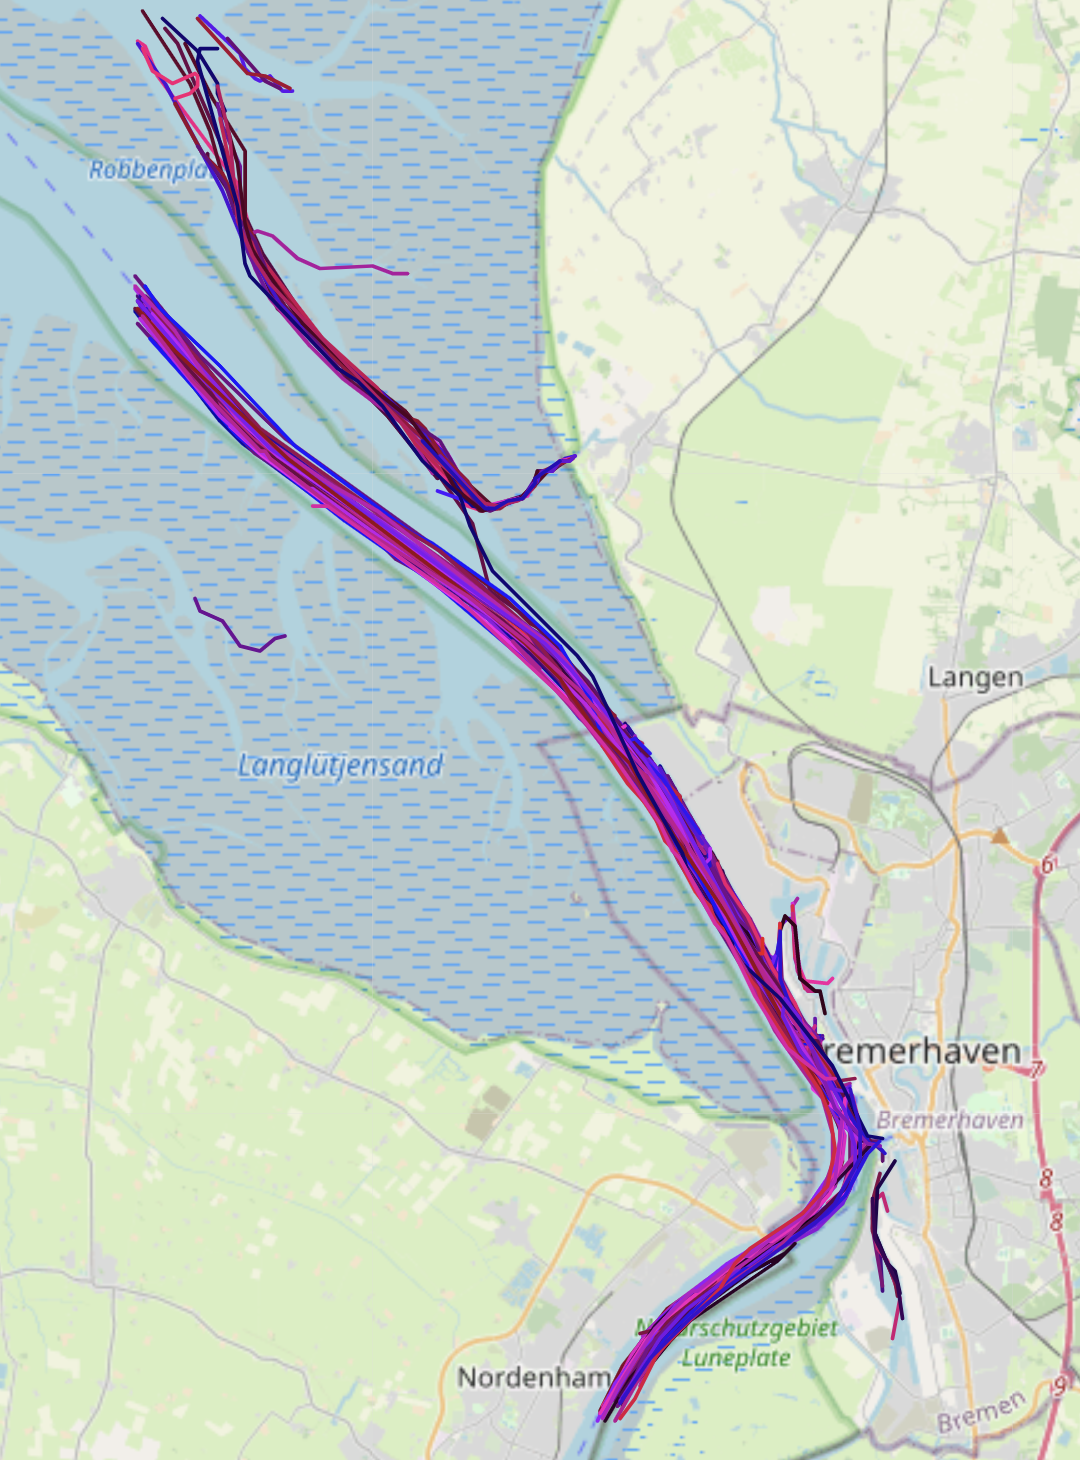
\includegraphics[width=0.5\textwidth]{images/ais/tracks/all_ships.png}
    \caption{System observation window and subset of the extracted trajectories.}
    \label{fig:tracks}
\end{figure}
    \subsection{The AIS-Environment}
    Recalling from chapter \ref{chap:synthetic} and the structure of the synthetic environment, the AIS environment differs from the simplified version by the underlying ground-truth data not being generated by arbitrary functions but from present instances of AIS records. The current state is defined by the signal recorded at $t$ while the desired action values are part of the next record at $t+1$. We will not add any additional features, resulting in a state representation that is semantically identical to $S3$ as defined in Eq. \ref{stateRepresentation} in subchapter \ref{subchap:variants}.
\par
For the final state representation, we defined two different variants. One instance uses the raw values of course over ground (COG) and speed over ground (SOG) whereas the second representation includes the artificial values for direction and speed, calculated by solely considering consecutive locations of the ship. The assumption behind this calculation is that the original values might not be accurate enough to train on in order to compute a precise trajectory for the agent. Having a unified way to extract direction and speed from sequences of AIS locations, as well as the reverse computation for the purpose of determining the next position, should be a more feasible and authentic approach. The final state representations and possible action values are thus defined by Eq. \ref{eq:realStateRepresentation}. 
\newpage
To make it clear that the action values are different from features of the state space, we use the distinct terminology of "course" and "tempo".
\begin{equation}
\begin{aligned}
    S1 := S_t &= \{lon_t, lat_t, COG_t, SOG_t\}
\\
    S2 := S_t &= \{lon_t,lat_t, direction_t, speed_t\}
\\
    A1 := A_t &= \{course_t, tempo_t\}
    \end{aligned}
    \label{eq:realStateRepresentation}
\end{equation} 

Although the focus on imitation learning makes the crafting of a reward function obsolete, we still add a simple adoption from $R3$ (see \ref{eq:rewardFunctions}) to the AIS environment for the purpose of quickly performing test runs with DDPG. Here, the maximum distance in meters to receive a non-zero reward is set arbitrary to $\alpha=8000$.
\par
In general, the environment loads in the desired dataset ("cargo", "tanker" etc.) and converts it to a list of trajectories. The list gets shuffled initially and also after every trajectory was presented to the agent in form of an episode. For every time step $t$, the environment calculates the next position of the agent by incorporating the proposed course and tempo of the given action. Additionally, the next GT position is set by the next entry of the trajectory and the reward gets calculated based on the distance between the agent and the GT position. All operations regarding the calculations of the next positions as well as the distance between two points on the globe is done with the library \textit{geopy} and its corresponding components \textit{distance} and \textit{destination}.
\par
Besides, we come up with an extended action space which additionally specifies the direction and speed of the agent when arriving at the calculated location. This is due to the fact that values for COG, SOG, direction and speed as given by the AIS message or the artificial extraction by MovingPandas have their semantic meaning just for the snapshot of the current state. The course and tempo that the agent proposes in order to get to the next position are distinct from the next direction and speed values that are present on exactly this new position. To compensate for the difference between the course taken and the final direction at the next position, we also force the agent to manually set the next direction and speed as it learns those values from the ground-truth data. Formally, we defined these possible actions in Eq.  \ref{eq:extendedAction}. Here, the optimal values for $next\_direction_t$ and $next\_speed_t$ are identical to $COG_{t+1}$ and $SOG_{t+1}$ of the state space (respectively $direction_{t+1}$ and $speed_{t+1}$).
\begin{equation}
\begin{aligned}
    A2 := A_t &= \{course_t, tempo_t, next\_direction_t, next\_speed_t\}
    \end{aligned}
    \label{eq:extendedAction}
\end{equation} 

Figure \ref{fig:explanation} illustrates the idea of the extension to the action space and the apprehension that the previous definition of $A1$ in Eq. \ref{eq:realStateRepresentation} might be ineligible. 
\begin{figure}[H]
    \centering
    \includesvg[width=0.7\textwidth]{images/thesis_A_B.svg}
    \caption{Difference between the values the agent has to submit (course) in order to reach the next ground-truth position (red arrows) and the direction as given by ground-truth (black arrows). The agent "learns" from the direction values of the training data, but has to suggest different values to reach the next point.}
    \label{fig:explanation}
\end{figure}


The graphic shows that in order to reach point B from point A, the agent has to submit suitable action parameters in course and speed. Here, the course value needed to reach Point B is illustrated by the red arrow. If the agent chooses the correct values, it will end up exactly at point B, but its values for direction and speed for the deriving next state do not match the values defined by the GT dataset and the AIS signals (indicated by the black arrows) because the computation of the next location is purely based on straight lines. When constructing a state space exclusively of longitude and latitude, this would not be an obstacle. However, in our case the agent is unable to fully reach the next state (position, direction, and speed) even when proposing the optimal action, hence the need for supplementary action values.
    \subsection{Results}
    \subsection{Tracing Failure}
    The previous chapter revealed that the proposed system of the designed environment and the usage of behavioral cloning did not produce feasible predictions. In this chapter, we will investigate two condensed experimental setups. The first one concentrates on the reproduction of a single ship trajectory, while the other one studies the influence of a second trajectory getting added. Here, the agent is not confronted with the task of generalization, in the sense that there is no test set and consequently no states that it did not encounter before. The conducted experiments are meant to confirm the correctness of the implementation (e.g., transition dynamics, bugs etc.), the ability of behavioral cloning to handle real world trajectories in contrast to the synthetic functions of chapter \ref{chap:synthetic} and especially the impact of different network architectures.
\par
First, it should be noted that there can potentially be a huge difference in the calculated performance and the empirically performance based on the form of the tracks as displayed in the upcoming figures. Our performance metric is derived from the euclidean distances, whereas the empirical performance of the final snapshot is best calculated by the dynamic time warping distance (DTW), first introduced by \cite{1104847}. One example being the instance where the agent perfectly generates the form of the path, but constantly lacks behind the ground-truth position due to a lower value in speed. The overall performance would be bad, but the resulting figures of the proposed tracks would look accurate.
\par
The upcoming figures display the prediction of the agent in red and the ground-truth in black. Being sampled from the "tanker"-dataset, this single trajectory contains 111 steps and thus spans a time horizon of approximately 18 minutes in the real world. Expert demonstrations only include this trajectory while the intern policy network of behavioral cloning is trained for $50$ epochs, with a learning rate of $\alpha = 1e^{-6}$ and a batch size of $4$. The focus of the different runs is on the network architectures which are specified underneath every panel of Fig. \ref{fig:singleTrack}. Mean distances are defined by $M$ in the subcaptions, while the x and y axes represent longitude latitude respectively.
\begin{figure}[H]
     \centering
     \begin{subfigure}[b]{0.48\textwidth}
         \centering
       \includesvg[width=\textwidth]{images/ais/single_line/mean_distance=127_SINGLE__batch=4_net=[4, 4]_steps=50_lr=1e-06.svg}
         \caption{$M=127 \quad [4-4]$}
         \label{fig:single1}
     \end{subfigure}
     \hfill
     \begin{subfigure}[b]{0.48\textwidth}
         \centering
             \includesvg[width=\textwidth]{images/ais/single_line/mean_distance=225_SINGLE__batch=4_net=[256, 128, 64]_steps=50_lr=1e-06.svg}
         \caption{$M=225 \quad [256-128-64]$}
         \label{fig:single2}
     \end{subfigure}
\end{figure}
\begin{figure}[H]\ContinuedFloat
     \begin{subfigure}[b]{0.48\textwidth}
         \centering
             \includesvg[width=\textwidth]{images/ais/single_line/mean_distance=282_SINGLE__batch=4_net=[16]_steps=50_lr=1e-06.svg}
         \caption{$M=282 \quad [16]$}
         \label{fig:single3}
     \end{subfigure}
          \hfill
     \begin{subfigure}[b]{0.48\textwidth}
         \centering
             \includesvg[width=\textwidth]{images/ais/single_line/mean_distance=2081_SINGLE__batch=4_net=[100]_steps=50_lr=1e-06.svg}
         \caption{$M=2081 \quad [100]$}
     \end{subfigure}
\end{figure}
\begin{figure}[H]\ContinuedFloat
         \begin{subfigure}[b]{0.48\textwidth}
         \centering
             \includesvg[width=\textwidth]{images/ais/single_line/mean_distance=1250_SINGLE__batch=4_net=[256, 128]_steps=50_lr=1e-06.svg}
         \caption{$M=1250 \quad [256-128]$}
         \label{fig:single5}
     \end{subfigure}
          \hfill
     \begin{subfigure}[b]{0.48\textwidth}
         \centering
             \includesvg[width=\textwidth]{images/ais/single_line/mean_distance=7182_SINGLE__batch=4_net=[512, 10]_steps=50_lr=0.0001.svg}
         \caption{$M=7182 \quad [512-10]$}
     \end{subfigure}
     \caption{Task of reproducing a single real-world vessel trajectory (overfitting). The y-axes and x-axes represent latitude and longitude values, respectively. $M$ indicates the average euclidean distance, whereas the numbers in brackets stand for the numbers of neurons in each hidden layer.}
     \label{fig:singleTrack}
\end{figure}

The first important discovery is that the implementation in terms of, e.g., transition dynamics is correct, since the proposed trajectories of the agent in Figs. \ref{fig:single1} and \ref{fig:single2} show significant overlap with the ground-truth. In this context, the policy network memorized the mapping from states to actions as given by the expert demonstrations. The intern calculation of the next geographic location of the agent in the environment does indeed seem to be an accurate inverse function of the artificial direction and speed values calculated during the creation of the dataset.
\par
Secondly, the network architecture that yielded the best results in the synthetic experiments of chapter \ref{chap:synthetic} and was also used for the first approach to the AIS datasets ($n_h^1=256, n_h^2=128, n_h^3=64$), performs exceptional well when confronted with the single trajectory (Fig. \ref{fig:single2}). Though, the best result of $M=127$ is set by a minimal network of $n_h^1=4$ and $n_h^2=4$, matching the number of input and output features.
\par
The importance of the proportion between the first and second hidden layer can be seen in the remaining panels. Removing just the third layer of the successful network of \ref{fig:single2} ends up with a drastic decline in performance to $M=1250$ (see \ref{fig:single5}). In general, the higher the amount of neurons in the first layer and the reduction in number of the second layer, the worse is the performance. Additionally, increasing the complexity of the network in terms of adding a fourth layer or upping the number of neurons does not necessarily yield better performance. This does seem surprising because we made the assumption that a complex network would simply overfit, but that is not the case. A complete list of all conducted experiments to the single trajectory reproduction can be found in the appendix and subchapter \ref{appendix:single}.
\par
After carrying out the experiments involving a single trajectory and the finding that it is certainly possible to generate a real world vessel path, we take it further by adding a second trajectory to the expert demonstrations. Works from \cite{edgardo} and \cite{martinsen2018curved} concentrate on a family of curves or ship paths that all move in the same direction. However, one requirement for our system is the extension to arbitrary moving ships without the restriction of predefined movement patterns. In this regard, a hypothesis is that a single network and policy is not capable of handling this flexibility and the opposing ship lanes and maneuvers.
\par
The following Fig. \ref{fig:double} shows a subset of the series of experiments ran with a learning rate of $\alpha=1e^{-6}$, increased training times ($50$ to $500$ epochs) and a batch size of $4$ and $8$. Every row of panels can be seen as one experiment where the two trajectories are split up. The left trajectory (A) starts from the middle and moves south-east, whereas the right trajectory (B) is the same one as used in the previous experiments, starting near the center and moving north-west. All results to this specific experiment can be found in the appendix, in subchapter \ref{appendix:double}.
\begin{figure}[H]
     \centering
     \begin{subfigure}[b]{0.48\textwidth}
         \centering
             \includesvg[width=\textwidth]{images/ais/double_line/b4_net_256_128_64_steps300_lr06_mean_distance=5779.svg}
         \caption{$M=5779  \quad [256-128-64]$}
         \label{fig:double3}
     \end{subfigure}
          \hfill
               \begin{subfigure}[b]{0.48\textwidth}
         \centering
             \includesvg[width=\textwidth]{images/ais/double_line/b4_n256_128_64_steps300_lr06_mean_distance=550.svg}
         \caption{$M=550 \quad [256-128-64]$}
         \label{fig:double4}
     \end{subfigure}
\end{figure}
\begin{figure}[H]\ContinuedFloat
     \begin{subfigure}[b]{0.48\textwidth}
         \centering
       \includesvg[width=\textwidth]{images/ais/double_line/b8_n1024_512_256_steps500_lr06_mean_distance_1430.svg}
         \caption{$M=1430  \quad [1024-512-256]$}
         \label{fig:double1}
     \end{subfigure}
     \hfill
     \begin{subfigure}[b]{0.48\textwidth}
         \centering
             \includesvg[width=\textwidth]{images/ais/double_line/b8_n1024_512_256_steps500_lr06_mean_distance=3453.svg}
         \caption{$M=3453  \quad [1024-512-256] $}
         \label{fig:double2}
     \end{subfigure}
\end{figure}
\begin{figure}[H]\ContinuedFloat
     \begin{subfigure}[b]{0.48\textwidth}
         \centering
             \includesvg[width=\textwidth]{images/ais/double_line/b8_n8_16_32_16_8_steps50_lr06_mean_distance=365.svg}
         \caption{$M=365 \quad [8-16-32-16-8]$}
         \label{fig:double5}
     \end{subfigure}
               \hfill
     \begin{subfigure}[b]{0.48\textwidth}
         \centering
             \includesvg[width=\textwidth]{images/ais/double_line/b8_n8_16_32_16, 8_steps50_lr06_mean_distance=398.svg}
         \caption{$M=398 \quad [8-16-32-16-8]$}
         \label{fig:double6}
     \end{subfigure}
     \caption{Task of reproducing two real-world vessel trajectories (overfitting). The y-axes and x-axes represent latitude and longitude values, respectively. $M$ indicates the average euclidean distance, whereas the numbers stand for the numbers of neurons in each hidden layer.}
     \label{fig:double}
\end{figure}

The first row, including Fig. \ref{fig:double3} and \ref{fig:double4}, displays the behavior of the prominent network $n_h^1=256, n_h^2=128, n_h^3=64$ which successfully learned to reproduce the synthetic curves and the single ship trajectory. Fig. \ref{fig:double4} shows that it is still capable of generating the trajectory of the previous experiment, but fails in case of the second presented trajectory with an average distance of $5779$ meters. Looking closer, we notice that the agent starts by following the path in the south-east direction when it abruptly decides to turn around. This turn is initiated almost at the exact location where trajectory B starts. We conclude that the network overfits to trajectory B and the input features are not evaluated granularly enough. Moving close to states of trajectory B while generating trajectory A forces the agent to start imitating trajectory B.
\par
In the second row, we see similar behavior but with the opposing track being overfit. While the agent in Fig. \ref{fig:double1} learns the form of the path but initially moves too fast, it fails  the task of generating trajectory B. The overall increase of neurons by the factor of $4$ does not show any significant improvement. However, a deviating network architecture of five layers and a structure of $n_h^1=8, n_h^2=16, n_h^3=32, n_h^4=16, n_h^5=8$ does show that a single neuronal network is able to memorize two distinct trajectories as displayed in Fig. \ref{fig:double5} and \ref{fig:double6}. Supplementary experiments with this kind of structure show worsening performance as the number of neurons increase. Nevertheless, even the best performing setup has an average distance of 381 meters, which is still unpractical for a system that tries to prevent collisions (we defined an arbitrary threshold of less than 50 meters while the inaccuracy of the AIS signal into consideration). In addition, this network architecture shows worse results than the initial round of experiments of subchapter \ref{subchap:aisResults} for the "big ships"-dataset. The average euclidean distance throughout all trajectories is $2593 \pm 3027$ with a median value of $1071$ (compared to $2136 \pm 2862$ and a median of $707$). Figure \ref{fig:finalBarPlot} demonstrates that a big chunk of previously good prediction ($<500$ meters) in Fig. \ref{fig:plotBig} moved into the next bucket of mediocre prediction of $500$ to $1000$ meters. 
\begin{figure}[H]
    \centering
    \includesvg[width=0.7\textwidth]{images/ais/bar_plots/big_ships_speed_10secs_scaled_NEW_APPROACH_8,16,32,16,8-steps7.svg}
    \caption{Histogram of trajectory performances. Network architecture $n_h^1=8, n_h^2=16, n_h^3=32, n_h^4=16, n_h^5=8$; $\alpha=1e^{-6}$; trained for $10$ epochs.}
    \label{fig:finalBarPlot}
\end{figure}

Generally speaking, the overall approach is too fragile. Changing the network architecture just slightly can cause catastrophic failure. The task of overfitting to a problem seems unnecessary, but the main idea behind those experiments is that, if a network is unable to overfit to the data, then it will certainly fail to generalize it well. All conducted experiments described in the last two subchapters and listed in the appendix lead to the conclusion that the building of a concrete system that is capable of learning representative vessel trajectories is unsuccessful. Still, we will provide possible improvements to the systems and describe pitfalls in the next subchapter that future investigation should account for.
    \subsection{Possible Improvements}
    Due to time constrains, it is not possible to test every single hypothesis and assumption. However, we will share our experience, uncertainties, and ideas in this subchapter to make them visible for scientist dealing with the same kind of topic.
\par
First, we would like to focus on the specific values of state and action space. The input features consist of values derived from the AIS signal, e.g., latitude and longitude. One problem with those values is that just small changes in the fractional digits result in big changes to the true position. Even though, we scaled the values for latitude and longitude to 0-1, the observation space might be too big ($25km /times 14.5km$) and thus causing inaccurate predictions purely based on fractional digits. One suggesting is that multiple models should be trained that are responsible for much smaller areas, leading to bigger differences in decimal places of the input features. Also, the use of a "Standardscaler" could be beneficial which causes the individual features to have a mean of 0 and a standard deviation of 1.
\par
Another assumption is that the features space does not cover up all potential influences to the controls taken by the captain. If we rightfully assume that the current heavily influences the motion patterns and controls of ships, than excluding this information from the feature space makes it impossible for the agent to learn an optimal policy. The underlying causality is missing. A possible next step is the extension of the state space with features like wind condition and tide information.
\par
Although the desired destination of a ship has to be defined manually and therefore was not included in the state space, it should be up to test if adding multiple features with regard to the distance or direction to the goal causes any improvements or makes classical interactive reinforcement learning practical as well. In theory, the destination can also be added artificially by simply extracting the last location of every trajectory.
\par
Last but not least, the usage of different network models e.g., transformers or generative adversarial networks could be tested as well. The vanilla approach of behavioral cloning simply makes use of a fully connected network.
 
\newpage   
\section{Conclusions}\label{chap:conclusions}
\newpage
\section{Future Work}



